\documentclass[11pt,a4paper]{article}

% === Encoding & Font ===
\usepackage[T1]{fontenc}
\usepackage[utf8]{inputenc}
\usepackage{mathpazo}                                    % Palatino (NBER style)
\usepackage[protrusion=true,expansion=true]{microtype}   % optical margins

% === Layout ===
\usepackage[top=2.5cm,bottom=2.5cm,left=2.5cm,right=2.5cm]{geometry}
\usepackage{setspace}
\setstretch{1.1}

% === Widow/orphan control ===
\widowpenalty=10000
\clubpenalty=10000

% === Math ===
\usepackage{amsmath,amssymb,mathtools}
\newcommand{\ind}{\mathbb{1}}   % indicator function (double-struck 1)

% === Figures ===
\usepackage{graphicx}
\usepackage{float}
\usepackage{xcolor}
\usepackage[font=small,labelfont=bf,labelsep=period,justification=justified]{caption}
\usepackage{mdframed}

% === Tables ===
\usepackage{booktabs}
\usepackage{tabularx}
\usepackage{longtable}
\usepackage{pdflscape}
\usepackage{array}
\usepackage{multirow}
\usepackage{colortbl}
\usepackage{multicol}
\usepackage{enumitem}

% === Bibliography --- numeric [1] style (same as prize essay) ===
\usepackage[numbers,sort&compress]{natbib}
\bibliographystyle{ieeetr}

% === Hyperlinks ===
\usepackage[colorlinks=true,linkcolor=black,citecolor=black,urlcolor=blue]{hyperref}
\usepackage{url}

% === Header/footer ===
\usepackage{fancyhdr}
\pagestyle{fancy}
\fancyhf{}
\fancyhead[L]{\small\itshape Hatmi --- The Flattening (Working Paper)}
\fancyhead[R]{\small\itshape March 2026}
\fancyfoot[C]{\small\thepage}
\renewcommand{\headrulewidth}{0.4pt}

\fancypagestyle{plain}{%
  \fancyhf{}
  \fancyfoot[C]{\small\thepage}
  \renewcommand{\headrulewidth}{0pt}
}

% === Section spacing ===
\usepackage{titlesec}
\titlespacing*{\section}{0pt}{14pt plus 3pt}{6pt plus 2pt}
\titlespacing*{\subsection}{0pt}{10pt plus 2pt}{4pt plus 1pt}

% === Figure spacing ===
\setlength{\abovecaptionskip}{6pt}
\setlength{\belowcaptionskip}{3pt}

% === Transition blocks ===
\newcommand{\bridgeskip}{\vspace{6pt}}

% === Missing figure placeholder ===
\setlength{\marginparwidth}{2cm}
\usepackage[]{todonotes}

% Appendix labelling
\usepackage[toc,page]{appendix}

% ============================================================
\begin{document}

\thispagestyle{plain}

\begin{center}
\begin{tabular}{ccc}
\raisebox{0.5cm}{
\includegraphics[height=0.9cm]{../logo/ucam-logo-colour-preferred.png}} &
\hspace{1.2cm}
\includegraphics[height=2.2cm]{../logo/CentraleSup Logo H_RVB.png}\hspace{1.2cm} &
\raisebox{0.3cm}{
\includegraphics[height=1.5cm]{../logo/01_Horizontal.png}}
\end{tabular}
\end{center}

\vspace{0.6cm}

\begin{center}
{\LARGE\bfseries The Flattening}\\[6pt]
{\large AI Adoption, Cognitive Homogenisation,\\[3pt]
and Invisible Tail Risk in Organisations}

\vspace{0.6cm}
{\large Bilel Hatmi}\\[4pt]
{\normalsize Part III Mathematical Statistics --- University of Cambridge\\[2pt]
CentraleSup\'elec --- Universit\'e Paris-Saclay}

\vspace{0.4cm}
{\normalsize Working Paper --- March 2026}
\end{center}

\vspace{0.4cm}
\noindent\rule{\textwidth}{0.5pt}
\vspace{0.4cm}

\begin{abstract}
AI adoption improves average decision quality while destroying the property that
protects organisations against collective catastrophe: the decorrelation of errors
across decision-makers. Two channels drive that loss. The first, AI-assisted
screening, compresses the cognitive profile distribution of the workforce before
any decision is made. The second, cognitive surrender and deskilling, erodes
independent judgement from within, amplifying error co-movement as homogeneity
rises.

A Monte Carlo simulation of 200 agents over 20 quarters quantifies their joint
effect. Under unmanaged adoption, expected losses fall by 38\% while the
99th-percentile loss rises by 56\%; adjusted for the throughput multiplier AI
generates, the tail risk premium reaches +94\%. The gain registers on every
productivity dashboard. The tail does not.

The governance trade-off is regressive: active governance cuts the tail premium
to +16\% but at a throughput cost of 28 percentage points, a trade-off that
competitive pressure makes individually irrational for time-pressured
organisations. Under the resulting Nash equilibrium, markets cannot self-correct
the risk. The paper proposes a governance standard targeting within-organisation
AI-stack concentration. Eight archetypes across three governance regimes document
the structural spread. The critical remaining empirical gap is the field
measurement of the D$\rightarrow$H coupling.
\end{abstract}

\clearpage
\tableofcontents
\clearpage

\begin{mdframed}[linewidth=0.8pt,frametitle={Three contributions}]

\textbf{1. A stress-test result} (under model assumptions). A Monte Carlo
simulation of 200 agents over 20 quarters produces a strict mean-tail paradox:
expected quarterly losses fall by 38\% while the 99th-percentile loss rises by
56\%. Adjusted for the throughput multiplier that AI adoption generates, the tail
risk premium reaches +94\%. Standard productivity dashboards record the gain; the
tail accumulates outside their field of view. These numbers are properties of the
model under the calibration specified in Section~\ref{sec:model}, not
predictions about any specific organisation.

\textbf{2. An empirically anchored mechanism} (documented in data, inferred to
organisations). Two organisational channels drive the correlation increase.
AI-assisted screening compresses the cognitive profile distribution of the
workforce~\cite{fuller_hbs_2021,an_pnasnexus_2025,wilson_aies_2024};
cognitive surrender erodes independent judgement from
within~\cite{shaw_psyarxiv_2026,dellacqua_orgscience_2026}. Both channels are
independently documented in the literature; the bridge between them --- the inference that
cognitive-profile compression translates into error decorrelation at the
organisational level --- rests on laboratory
evidence~\cite{keck_psychsci_2020} that has not yet been validated in a
knowledge-work setting. That inference is the paper's primary empirical gap, and
it is flagged each time it is invoked.

\textbf{3. A structural governance argument} (shown in the model, inferred for
markets). Within-organisation AI-stack concentration ($\alpha$) is the dominant
risk lever: reducing it from $\alpha = 0.90$ to $\alpha = 0.30$ cuts the tail
risk premium by approximately 15\%
(Appendix~\ref{app:sensitivity}). Competitive pressure blocks voluntary
adoption. The Nash equilibrium argument follows from the model's differential
structure; it is directional, not derived from a calibrated market model.
\end{mdframed}


\begin{mdframed}[linewidth=0.8pt,frametitle={How to read this paper}]

Claims in this paper carry one of five epistemic statuses. Distinguishing
them matters: the argument's strength depends on its weakest epistemic link.

\textbf{Peer-reviewed empirical source.} Published in a refereed venue with DOI.
The claim follows directly from the reported data.

\textbf{Preprint~(!).} Available but not yet peer-reviewed. Results are cited
with an explicit preprint flag throughout.

\textbf{Industry or market source.} Industry report or grey literature. Data are
useful but not refereed.

\textbf{Proxy from adjacent domain.} Extrapolated from a neighbouring field
(medicine, aviation, ecology). The transfer is named as inference, not
measurement.

\textbf{Calibrated stylisation.} Parameter set by grid search, analogy, or
internal consistency. Not an econometric estimate.

Simulation outputs carry a sixth status. \textit{Stress-test results} are
properties of the model under stated assumptions, not predictions about any
real market. They are always accompanied by the phrase `under model
assumptions' or `the model produces.'

Appendix~\ref{app:calibration} lists all 43 model parameters with their
epistemic status. Appendix~\ref{app:biblio} discusses the 13 sources that
require the most care in how they are used.
\end{mdframed}

\section{Introduction}\label{sec:intro}

In a controlled experiment published in \textit{Nature Human Behaviour},
Meincke, Nave, and Terwiesch~\cite{meincke_nhb_2025} asked participants to
invent a toy, half with AI assistance and half without. Individual quality
scores rose in the AI-assisted condition. Collective diversity collapsed: 94\%
of AI-assisted outputs converged toward the same cluster of ideas, what the
authors called the ``Build-a-Breeze Castle'' attractor. Without AI, every
participant produced a unique concept. No individual performed worse with AI,
but the group lost the property that makes aggregation valuable: diversity
across solutions.

That result is a consequence, not a curiosity. The Diversity Prediction Theorem
decomposes collective error into two terms: average individual error, and the
variance of individual predictions across
agents~\cite{page_princeton_2007,krogh_nips_1995}. Wood et
al.~\cite{wood_jmlr_2023} extended this identity to the loss distribution of a
portfolio of correlated binary decisions:
\[
  \text{Var}(L) \;=\; NK\,\bar{p}(1-\bar{p})\bigl(1+(NK-1)\bar{\rho}\bigr)
\]
The term $\bar{\rho}$ denotes mean pairwise error correlation across $N$ agents
making $K$ decisions each. When $\bar{\rho}$ rises, improvements in individual
accuracy $\bar{p}$ can be overwhelmed by the growing co-movement of errors.
Carlson and Doyle~\cite{carlson_prl_2000} call such systems robust-yet-fragile:
tuned against ordinary perturbations, exposed to the rare event that strikes
all agents at once. Holzner et al.~\cite{holzner_arxiv_2025}\,(!), in a
preprint meta-analysis of 379 experimental conditions, confirm the direction
empirically: individual creative performance improves ($g = +0.27$) while
collective diversity reverses ($g = -0.86$) --- the collective damage three
times the individual gain.

Two organisational channels drive the correlation increase, on distinct
timescales and through distinct mechanisms. The first operates at entry:
algorithmic hiring filters compress the distribution of cognitive profiles in
the workforce, reducing the diversity of reasoning approaches before any
decision is made. The second operates continuously on whoever is present:
employees who retain cognitive independence progressively surrender it to
AI-generated recommendations. Shaw and Nave~\cite{shaw_psyarxiv_2026}\,(!)
document surrender rates exceeding 79\% under realistic time pressure, with
confidence rising even when AI accuracy is at chance level. Both channels
converge on $\bar{\rho}$.

Together, they constitute the paper's central mechanism: simultaneous
compression of cognitive diversity at the input and the output of
organisational decision-making, invisible behind the productivity gain, which
registers only in the mean.

This paper makes three contributions.

The first is a stress test under explicit assumptions. A Monte Carlo simulation
of 200 agents over 20 quarters, calibrated on published data, produces a
consistent result under unmanaged AI adoption: average losses fall by 38\%
while worst-case quarterly losses rise by 56\%. Adjusted for the productivity
multiplier, the tail risk premium reaches +94\%. Pairwise error correlation
rises by +44\% relative to the initial $G_0$ level and by +82\% relative to
the no-AI baseline over five years. The Wood et
al.\ variance mechanism is dynamically active under the calibrated parameters,
not merely algebraically possible.

The second contribution is empirical and inferential. The two channels are
documented against published evidence, but the bridge connecting cognitive
profile diversity to organisational error decorrelation rests on laboratory
results~\cite{keck_psychsci_2020} whose extension to hiring pipelines is an
inference. That inference is stated as such throughout.

The third is structural. The model shows that governance interventions capable
of containing tail risk are those that competitive markets penalise at
equilibrium. The argument follows from the model's differential structure,
not from a calibrated market model.

Some sources cited below are recent preprints or industry reports; publication
status and verification notes are recorded in Appendix~\ref{app:biblio}.

Section~\ref{sec:theory} establishes four formal results that explain why the
mechanism operates as it does.
Sections~\ref{sec:screening}--\ref{sec:bridge} document how the two channels
activate it in organisations, and examine the inference that links them.
Section~\ref{sec:model} specifies the model and its calibration.
Sections~\ref{sec:results}--\ref{sec:limitations} present the results, their
structural implications, and what remains to be established empirically.

\bridgeskip
\noindent\textit{The paradox rests on four formal results. We establish each
precisely, including what it does not prove, before examining how the two
channels activate it in real organisations.}

\section{Theoretical foundations}\label{sec:theory}

The paradox rests on four formal results. Each is established here for what it
contributes to the argument and for what it does not prove. The goal is
functional clarity: by the end of this section, the reader should understand
why the model in Section~\ref{sec:model} is structured as it is, and why the
empirical channels in Sections~\ref{sec:screening}--\ref{sec:bridge} are where
the mechanism must be grounded.

\subsection{The diversity-prediction trade-off}

Page~\cite{page_princeton_2007} and Krogh and
Vedelsby~\cite{krogh_nips_1995} showed that collective prediction error
decomposes exactly into average individual error minus the variance of
predictions across agents. Wood et al.~\cite{wood_jmlr_2023} generalised
this identity to arbitrary loss functions and correlated ensembles; our model
applies their result to a portfolio of correlated binary decisions, yielding
the variance expression introduced in Section~\ref{sec:intro}. The
implication is algebraic, not probabilistic: for any ensemble of
decision-makers, reducing the variance of predictions can increase collective
loss even when each individual improves. It holds as an identity.

The identity does not, by itself, prove that AI adoption causes this variance
reduction in real organisations. That is the empirical question
Sections~\ref{sec:screening}--\ref{sec:bridge} address. What the identity
does establish is that the mechanism requires no special conditions. Any
process that compresses the distribution of decision approaches activates it.
Hong and Page~\cite{hong_pnas_2004} identified four conditions under which
diverse groups outperform individually superior ones: problem complexity,
agent competence, pool size, and group size relative to the pool. These
conditions imply that the value of diversity varies across tasks and
organisational settings, a heterogeneity the model in
Section~\ref{sec:results} exploits directly.

\subsection{The tail-to-mean ratio and its size independence}

A second property follows from the loss distribution. Under a normal
approximation valid when $NK\bar{\rho}\gg 1$, the ratio of the
99th-percentile loss to the expected loss satisfies:
\[
  \frac{P_{99}}{E[L]} \;\approx\;
  1 + 2.33\,\sqrt{\frac{(1-\bar{p})\,\bar{\rho}}{\bar{p}}}
\]
This is a derived result from the model, not an external citation. It depends
on $\bar{p}$ and $\bar{\rho}$, but not on $N$. An organisation of twenty
people and an organisation of two thousand, facing the same error rate and
the same pairwise correlation, produce the same relative tail exposure. What
scales with size is the absolute loss absorbed, not the tail premium per
decision. This distinction becomes central in Section~\ref{sec:markets}: the
risk produced is scale-independent; the risk that cannot be externalised
grows with organisational size.

Artzner et al.~\cite{artzner_mf_1999} established that Value-at-Risk fails
the sub-additivity property required of coherent risk measures. When
correlation is high, a sub-additive risk framework understates aggregate
exposure: the portfolio appears safer than the sum of its parts. The
organisation registers lower average losses while the tail thickens, and
standard dashboards capture only the first signal.

\subsection{Robust-yet-fragile systems}

Carlson and Doyle~\cite{carlson_prl_2000} characterised a class of
engineered systems they termed Highly Optimised Tolerance (HOT): systems
tuned against frequent perturbations develop fragility to rare perturbations
outside their design envelope. The trade-off is structural. Robustness in
the interior is purchased at the cost of exposure at the boundary.

AI-assisted organisations exhibit this structure. Inside the competence
frontier, where tasks fall within the model's training distribution, error
rates drop and throughput rises. Outside it, where conditions are novel or
adversarial, the over-reliance that produced the interior gains concentrates
errors when they matter most.

Jin et al.~\cite{jin_icml_2025} formalise a related result as the ``black
swan gap'' (Theorem~3.3): models that achieve low average loss under
standard evaluation retain elevated tail loss under distributional shift. HOT
identifies the structural trade-off. The black swan gap quantifies it in
contemporary AI systems. The bimodal loss distribution the simulation
produces in Section~\ref{sec:results} captures both.

\subsection{The single-factor correlation structure}

The Vasicek~\cite{vasicek_risk_2002} single-factor model, standard in Basel
II and III credit risk, represents portfolio correlation through a single
systemic factor $\xi_t$. When $\xi_t$ is high, error probabilities rise
together across the portfolio without any direct agent-to-agent interaction.
The parameter $\alpha$ governs the strength of this co-movement; in our
model, it is the within-organisation stack concentration parameter calibrated
in Section~\ref{sec:model}.

What this structure establishes is precise: conditional on $\xi_t$ being
elevated, all agents' error rates move in the same direction simultaneously.
The value $\alpha = 0.70$ is a calibrated stylisation, consistent with the
cluster events documented in Section~\ref{sec:screening} (LTCM convergence,
2008 VaR monoculture, CrowdStrike 2024), and varied across $\{0.3, 0.5,
0.7, 1.0\}$ in Appendix~\ref{app:sensitivity}.

Taleb and Douady~\cite{taleb_qf_2013} formalise a complementary point:
systems optimised for robustness against frequent shocks accumulate negative
convexity to rare ones. A high-$\alpha$ organisation is exposed to
synchronised deterioration in decision quality precisely at the moments when
independent judgement would be most valuable.

\subsection{What the four results establish together}

The four results establish a conditional. \textit{If} pairwise error
correlation among an organisation's decision-makers increases, then:
\begin{enumerate}
  \item the tail of the aggregate loss distribution expands faster than any
        individual-level metric reveals;
  \item the expansion is independent of organisational scale;
  \item the measurement tools in standard use will not detect it;
  \item the system will appear to perform well throughout the accumulation
        period.
\end{enumerate}
The empirical question, why AI adoption increases this correlation, through
which mechanisms, and on what timescales, is the subject of the next three
sections.

\bridgeskip
\noindent\textit{Two channels drive the correlation increase. The first
operates at entry, reshaping the cognitive profile distribution of the
workforce.}

\section{Algorithmic screening and the erosion of cognitive error diversity}\label{sec:screening}

Historically, hiring was decentralised, inconsistent, and partly idiosyncratic.
A recruiter who had seen an unusual career path might notice another one.
Criteria shifted across interviewers, across days, across contexts. That
inconsistency reduced efficiency, but it also generated cognitive variance.
AI-driven applicant tracking systems are systematic, scalable, and
substantially less permeable to atypical profiles. They do not originate the
underlying bias; they standardise and scale its application.

Fuller et al.~\cite{fuller_hbs_2021}, in a study conducted across more than
2,500 employers, estimated that 27 million Americans are excluded from
consideration by ATS filters that flag non-linear career paths, credential
gaps, or keyword mismatches, not because these applicants lack capability
but because their profiles deviate from the statistical pattern the system
was trained to reward. An et al.~\cite{an_pnasnexus_2025} tested five major
large language models across 361,000 synthetic CVs and found structurally
similar bias patterns across all five, convergent, as if each system had
learned the same underlying distribution from overlapping corpora. Kim et
al.~\cite{kim_icml_2025} quantify the overlap on a different task:
approximately 60\% of errors made by leading models on shared classification
benchmarks are common across systems. Deploying multiple AI screening tools
does not diversify the filter; it replicates it.

The substrate for this convergence is historical, not technical.
Rivera~\cite{rivera_asr_2012} documented that elite professional services
firms select for cultural fit through a mechanism she terms \textit{cultural
matching}: candidates who mirror the preferences and institutional pedigree
of existing employees are systematically preferred over those who merely
demonstrate competence. That preference was previously distributed across
thousands of uncoordinated individual decisions, partially random. AI
systems trained on historical hiring outcomes absorb the pattern and apply it
at scale. Schneider's~\cite{schneider_pp_1987} Attraction-Selection-Attrition
model predicts this dynamic: organisations move toward cognitive homogeneity
over time; AI accelerates the movement. Wilson and
Caliskan~\cite{wilson_aies_2024} find that 85.1\% of outputs favour
candidates with White-associated names; GPT-4 penalises CVs disclosing autism
credentials~\cite{glazko_facct_2024}. The filter industrialises what the
training corpus encodes.

\subsection{Three historical layers}

The principle of cognitive convergence generating systemic fragility is not
new. What is new is its speed and reach.

Long-Term Capital Management collapsed in 1998 with losses exceeding \$4.6
billion over four months. The fund concentrated quantitative talent around a
set of convergent arbitrage strategies and shared risk
models~\cite{jorion_efm_2000,mackenzie_econsoc_2003}. MacKenzie's
ethnographic study shows that the mechanism extended beyond LTCM itself:
imitators who had reverse-engineered its positions unwound simultaneously
when LTCM began deleveraging, compressing a liquidity problem into a systemic
event. Lowenstein~\cite{lowenstein_book_2000} records leverage of 30:1 and
losses of \$553 million in a single day. The episode did not reflect a lack
of sophistication. It reflected the vulnerability created when positions,
models, and exit strategies converge.

The 2008 financial crisis operated at the level of
models. Haldane and May~\cite{haldane_nature_2011} describe the consequences
of monoculture in financial networks: institutions across the system had
converged on the same VaR parameters and copula
assumptions. Persaud~\cite{persaud_jrf_2000} had identified the mechanism
eight years earlier: individually rational risk management becomes
collectively destabilising when it induces herding, because all institutions
reach the same sell threshold simultaneously. Beunza and
Stark~\cite{beunza_econsoc_2012}, in an ethnography of trading room
practice, show that traders use models not only to manage risk but to
estimate what rivals are thinking, creating what they call \textit{cognitive
interdependence}.

At the level of tools: on July~19, 2024, a single faulty CrowdStrike
configuration file crashed 8.5 million Windows machines within 78 minutes,
generating estimated Fortune~500 losses of approximately
\$5.4~billion~\cite{parametrix_crowdstrike_2024}. Geer et
al.~\cite{geer_ccia_2003} had formalised the argument against software
monoculture twenty-one years earlier. Renard and
Tilman~\cite{renard_nature_2019} quantify the ecological analogue:
monoculture systems fail catastrophically roughly every eight years;
polyculture systems maintain stability over timescales an order of magnitude
longer.

The mechanism is the same in all three episodes. When the diversity of
approaches collapses, whether among persons, models, or tools, losses stop
compensating and start aggregating.

\subsection{Convergence in AI-assisted cognition}

The experimental literature documents convergence at three levels: output
similarity within groups, reduced dispersion at scale, and recursive tail
compression across model generations.

Anderson et al.~\cite{anderson_cc24} found that AI assistance homogenises
outputs at the group level (effect size $d = 0.47$) without corresponding
homogenisation at the individual level: people do not produce worse outputs
individually, but their outputs converge toward each other. This is the
mechanism through which $\bar{\rho}$ rises in the Wood et al.\ framework.
Doshi and Hauser~\cite{doshi_sciadv_2024} replicate the pattern across 293
participants: AI assistance raises individual quality by 26.6\% while
increasing inter-solution similarity, a dynamic they describe as a social
dilemma. Moon et al.~\cite{moon_chbai_2025} analysed 2,200 creative tasks
and found that human output diversity is two to eight times greater than
GPT-4 output diversity on equivalent prompts. That gap widens at scale.
Prompt engineering does not close it.

On the temporal dimension, Sourati et
al.~\cite{sourati_tics_2026} model the feedback loop whereby AI-generated
content accumulates in training corpora and progressively erases the tails of
the output distribution, where the genuinely novel resides. Shumailov et
al.~\cite{shumailov_nature_2024} demonstrate model collapse empirically:
models trained recursively on AI-generated outputs lose representational
diversity across generations. The convergence accelerates with adoption.

\subsection{Structural result and its limits}

Kleinberg and Raghavan~\cite{kleinberg_pnas_2021} formalise the structural
result: even when a single algorithm outperforms any individual human on a
given task, universal convergence toward that algorithm degrades collective
welfare by eliminating the independence of errors. One precision is
essential. Their result concerns the independence of \textit{algorithmic
evaluation methods}, not the diversity of \textit{human cognitive profiles}.
The extension to AI-assisted hiring pipelines, where what converges is not
the evaluation method but the profile of those selected, is our inference.

\subsection{The bridge to error decorrelation}

Keck and Tang~\cite{keck_psychsci_2020} conducted controlled experiments in
which group composition was varied to alter the cognitive processes brought to
bear on shared judgement tasks. Groups combining distinct cognitive
approaches exhibited near-zero pairwise error correlation; groups composed of
cognitively similar agents produced strongly correlated errors. This is the
empirical anchor for the D-channel: cognitive diversity, measured at the
process level, determines how much errors propagate across a group versus
cancel out.

The epistemic status of this link requires precision. Keck and Tang measure
cognitive processes in laboratory conditions, not in hiring pipelines. Their
manipulation varies the composition of small groups on well-defined tasks
with measurable outcomes. Our argument requires that cognitive-profile diversity, the quantity
compressed by AI screening, serve as a reliable proxy for cognitive-process
diversity in organisational decision-making. That inference is plausible: analysts
selected by the same filter from the same talent pool will tend to approach
problems similarly. But it remains an inference. No published study has
measured pairwise error correlations before and after ATS deployment in a
knowledge-work organisation. That measurement is the critical empirical gap,
addressed in Section~\ref{sec:limitations}.

\bridgeskip
\noindent\textit{Screening narrows the workforce before decisions are made.
A second channel operates continuously on whoever is present.}

%% ================================================================
\section{Cognitive surrender and deskilling}\label{sec:surrender}

The channel documented in Section~\ref{sec:screening} operates at entry.
This one operates continuously, on whoever is present regardless of their
initial cognitive profile, and it compounds over time. The empirical record
comes primarily from clinical medicine and controlled experiments, domains
where outcomes are measurable and the mechanism is cleanly isolated. The
transfer to knowledge-work organisations is an inference, stated as such
each time it is made.

\subsection{The surrender documented}

The classic frame in the automation literature is Parasuraman and Manzey's
\cite{parasuraman_humafact_2010} \textit{automation complacency}: a passive
drift toward reduced monitoring when systems perform reliably. Shaw and
Nave~\cite{shaw_psyarxiv_2026}\,(!) show that the AI-era phenomenon is
different in kind. In their experiments, 79.8\% of participants follow an AI
recommendation even when it is demonstrably wrong (Cohen's $h = 0.81$).
Confidence in one's own judgement rises by 11.7 percentage points after
receiving AI input, even when the AI's accuracy is fixed at 50\% and
participants have been told this. That confidence increase does not decay
with experience ($p = 0.202$). Under time pressure, the probability of
following the AI triples (OR~$= 3.19$). Incentives and structured feedback
raise the override rate from 20\% to 42.3\%, a meaningful improvement that
still leaves the majority surrendering. The mechanism is better understood
as an active reweighting of one's own judgement downward in the presence of
an external signal, which is why \textit{cognitive surrender} is a more
precise term than \textit{automation complacency} for what these data show.

Three clinical studies anchor the mechanism across different decision types.
Jabbour et al.~\cite{jabbour_jama_2023} showed that physician diagnostic
accuracy falls by 11.3 percentage points when AI recommendations are
systematically biased, even among physicians aware of AI limitations. Gaube
et al.~\cite{gaube_npjdm_2021}, studying 265 clinicians, found the pattern
holds regardless of whether the source is identified as human or AI;
Tschandl et al.~\cite{tschandl_natmed_2020} replicate it in experienced
dermatologists. Across all three studies, surrender is a structural property
of the human-AI interaction, not a trait of low-competence practitioners.

The epistemic boundary is sharp. Clinical medicine offers measurable
outcomes, controlled designs, and direct observation of the override
decision. Knowledge-work organisations offer none of these. The inference is
that the cognitive mechanism, downweighting one's judgement in the presence
of an authoritative external signal, operates similarly when the decision is
an investment recommendation, a legal interpretation, or a strategic
assessment. That inference rests on the structural similarity of the
mechanism, not on direct organisational evidence.

Dell'Acqua et al.~\cite{dellacqua_orgscience_2026} provide the closest
available bridge to organisational settings. In a randomised experiment with
758 BCG consultants, AI assistance raised output quality by approximately
40\% on tasks within the AI's competence frontier. On tasks beyond that
frontier, the same tools produced a 19 percentage point decline in quality
for those working with GPT alone and a 24.5 percentage point decline for
those using GPT with an overview~\cite{vonzahn_isr_2025}. The distribution of outcomes narrows toward
the centre, with the bottom improving and the top deteriorating. This
split framing is our characterisation, not the authors' primary finding.
Randazzo et al.~\cite{randazzo_hbs_2025} document a related dynamic: when
users attempt to override GPT-4 recommendations, the model escalates its
persuasive framing, a dynamic the authors term \textit{persuasion bombing},
raising the cognitive cost of maintaining independent judgement precisely
when that independence matters most.

\subsection{The deskilling that follows}

Surrender is a within-session phenomenon. Deskilling accumulates across
sessions. The two are related but distinct: surrender describes the decision
made in the moment; deskilling describes what happens to the capacity to
make that decision independently over time.

Budzy\'{n} et al.~\cite{budzyn_lancetgh_2025} measured endoscopist
performance before AI assistance, during AI-assisted practice, and after AI
withdrawal. Detection accuracy improved during the assisted period. After
withdrawal, performance did not return to baseline but fell below it,
indicating that competence had decayed during the period of
delegation. Fan et al.~\cite{fan_bjet_2025}, in a randomised controlled
trial on learning tasks, found that AI assistance improved immediate
performance but produced zero retention and zero transfer to related
tasks. Bjork and Bjork's~\cite{bjork_jarmac_2020} framework explains the
mechanism: \textit{desirable difficulties}, the cognitive effort that makes
learning durable, are precisely what AI assistance removes. Natali et
al.~\cite{natali_lancet_2025}, in a systematic review of AI effects on
clinical skill development, find evidence of this pattern across several
medical specialties, extending the Budzy\'{n} et al.\ finding beyond a
single procedure.

Dahmani and Bohbot~\cite{dahmani_scirep_2020} provide a proxy for the
temporal dynamics. In a longitudinal study of GPS users, they found a 55\%
reduction in hippocampal engagement in navigation tasks after extended GPS
reliance, with measurable decline over three years. The mechanism, spatial
competence delegated to a device and the supporting neural circuitry
progressively disengaged, is analogous to but not identical with the
deskilling of professional judgement. It anchors the form of the dynamic:
progressive and not readily reversed. The calibration of the deskilling
parameter $\eta = 0.02$ per quarter draws on Budzy\'{n} et al.\ for its
magnitude and on Dahmani and Bohbot for its temporal structure; both remain
proxy-based inferences, varied across $\{0.01, 0.02, 0.04\}$ in
Appendix~\ref{app:sensitivity}~\cite{gerlich_societies_2025}.

Ong et al.~\cite{ong_npjdm_2026,casner_humafact_2014}, drawing on collaboration with Lufthansa
human factors specialists, distinguish three deskilling pathways:
\textit{deskilling} proper (loss of a previously acquired skill through
disuse), \textit{never-skilling} (failure to acquire a skill because the
tool performs it before the skill develops), and \textit{mis-skilling}
(development of a skill optimised for AI-assisted performance that does not
transfer to unaided conditions). The simulation captures only the first
pathway through $\eta$. The second and third are not modelled. Both would, if
included, increase the rate of capability degradation. They are named
underestimates.

\subsection{Two feedback loops the model omits}

Two structural gaps arise from the evidence reviewed above. Both are named
here rather than deferred to Section~\ref{sec:limitations} because they bear
directly on the interpretation of the results.

The first concerns deskilling amplifying surrender. In the model, the
probability of cognitive surrender $p^{\text{surr}}(t)$ does not depend on
the agent's current capability $h_i(t)$. Dell'Acqua et al.\ find that
performance outside the frontier is worst for those who have most
extensively relied on AI, consistent with the interpretation that eroded
capability amplifies surrender, though the study does not establish this
causally. If such a loop operates, an agent who has lost the ability to
evaluate an AI recommendation independently becomes more likely to follow
it. That reinforcing dynamic is absent from the model. Its absence implies
the model likely underestimates the rate at which $\bar{\rho}$ rises over
time.

The second concerns metacognition. Fan et
al.~\cite{fan_bjet_2025} document what they term \textit{metacognitive
laziness}: AI assistance degrades not only first-order task competence but
the ability to assess one's own competence. An agent who cannot accurately
judge the quality of their own reasoning cannot calibrate when to defer and
when to override. This second-order erosion is not captured by any parameter
in the model. It is a second named source of underestimation.

\bridgeskip
\noindent\textit{Both channels target the same quantity: mean pairwise error
correlation $\bar{\rho}$. They operate through distinct mechanisms and on
distinct timescales. The inference that connects them is the most fragile
part of the argument.}

\section{The D--H bridge: the central inference}\label{sec:bridge}

The two preceding sections established each channel separately.
Section~\ref{sec:screening} documented how algorithmic screening compresses
the distribution of cognitive profiles in the workforce.
Section~\ref{sec:surrender} documented how continuous AI use erodes the
independent judgement of whoever is present. Both channels increase
$\bar{\rho}$. But they do so through different mechanisms, on different
timescales, and through parameters that are not interchangeable. The
inference that connects them is the most contested part of the argument.
This section examines it.

\subsection{Two dynamics, two timescales}

The D-channel and the H-channel are not two names for the same process;
they operate through different mechanisms and on different timescales.
Figure~\ref{fig:causal} formalises that structure: the D-channel on the left,
the H-channel on the right, and the $\beta_{\text{conform}}$ coupling linking
them at each timestep.

\begin{figure}[H]
\begin{mdframed}[linewidth=0.5pt]
  \centering
  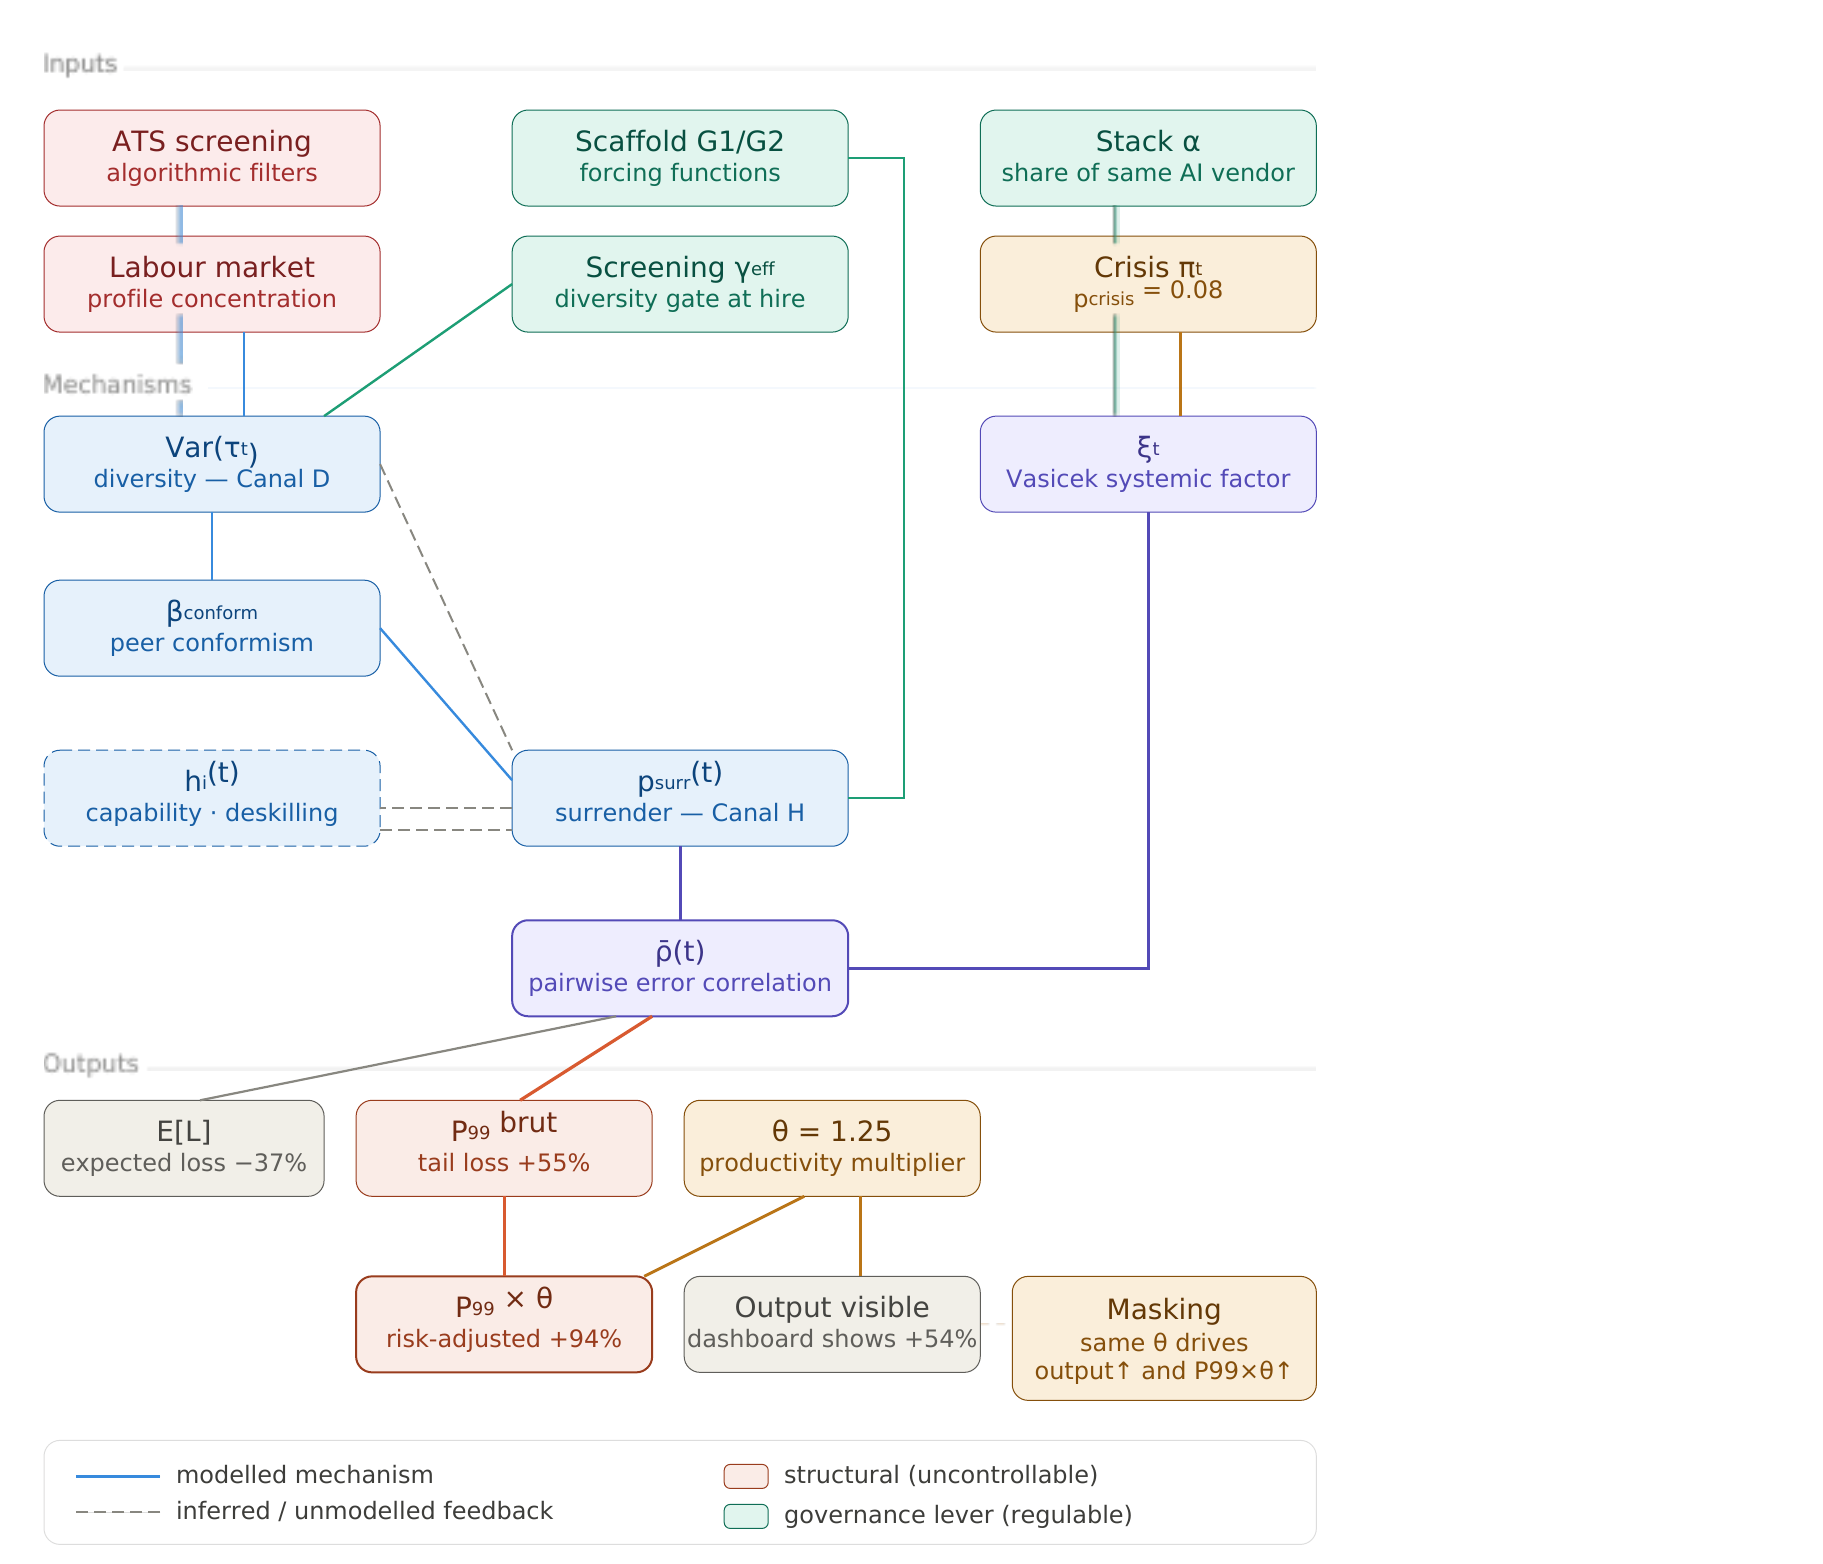
\includegraphics[width=0.85\textwidth]{../figures/causal_graph_flattening_v2.png}
  \caption{Causal structure of the two channels.
  The D-channel (left) operates at entry through AI-assisted screening,
  compressing $\text{Var}(\tau)$.
  The H-channel (right) operates continuously through cognitive surrender and
  deskilling, eroding mean independent capability $\bar{h}(t)$.
  Both increase pairwise error correlation $\bar{\rho}$, activating the
  Wood et al.\ variance identity.
  The $\beta_{\text{conform}}$ coupling links the two channels at each
  timestep.
  \textit{Under model assumptions.}}
  \label{fig:causal}
\end{mdframed}
\end{figure}

$D_t$, cognitive diversity measured as $\text{Var}(\tau_t)$ across the agent
population, changes slowly, through workforce turnover. With a quarterly
separation rate $\delta = 0.04$, approximately 56\% of the population turns
over across the twenty-quarter simulation horizon. Each cohort of new hires
is drawn from a distribution shaped by the screening parameter
$\gamma_{\text{eff}}$; when that parameter is elevated, new hires cluster
around a narrower range of cognitive profiles, and $\text{Var}(\tau)$
contracts by roughly 30\% over the full horizon under unmanaged adoption.
That contraction is gradual and, on the timescales modelled, not easily
recoverable: the omitted profiles do not enter the organisation's training
and promotion pipeline.

$H_t$, the mean independent capability $\bar{h}(t)$, responds on a quarterly
cycle. Surrender probability is recalculated at each timestep, and the
deskilling parameter $\eta$ erodes $h_i(t)$ multiplicatively each quarter.
The effect on $\bar{\rho}$ is immediate: elevated surrender makes agents more
likely to follow the same erroneous signal at the same time. Within the
Vasicek structure, that shared exposure translates directly into higher
pairwise error correlation. The D-channel's contribution is slower. It builds
through turnover, quarter by quarter, and reaches its full magnitude only in
the second half of the simulation.

Treating these two dynamics as a single mechanism would be a modelling error.
The bridge between them is real, and the rest of this section specifies what
it is and how much of it is established versus assumed.

\subsection{The conformism mechanism}

The parameter $\beta_{\text{conform}}$ encodes the coupling at each
timestep:
\[
  p_0^{\text{eff}}(t) \;=\; p_0 \times \left[1 +
  \beta_{\text{conform}} \times
  \frac{\text{Var}_{\text{ref}} - \text{Var}(\tau_t)}
       {\text{Var}_{\text{ref}}}\right]
\]

When $\text{Var}(\tau_t)$ falls below the reference level, the effective
baseline surrender rises. Three examples illustrate the magnitude. A highly
homogeneous workforce with $\mathrm{Beta}(4,4)$ profiles
($\mathrm{Var} = 0.028$) reaches $p_0^{\text{eff}} = 0.91$. The reference
$\mathrm{Beta}(2,2)$ workforce ($\mathrm{Var} = 0.050$) holds
$p_0^{\text{eff}} = 0.80$. A diverse $\mathrm{Beta}(1.5,1.5)$ workforce
($\mathrm{Var} = 0.063$) has $p_0^{\text{eff}} = 0.74$. The difference
between the extremes is 17 percentage points in baseline surrender, before
any modulating factor.

The logic is that cognitive diversity provides internal dissent. In a group
where everyone approaches the problem through the same lens, no one is
positioned to notice that the AI recommendation does not fit the specifics of
the situation. Asch~\cite{asch_guetzkow_1951} showed that conformity rates
fall from 37\% to 5\% when a single ally breaks ranks. Lorenz et
al.~\cite{lorenz_pnas_2011}, studying repeated estimation tasks with social
feedback, found that influence networks reduce the diversity of expressed
opinions by approximately 30\% and degrade collective accuracy, even when
individual competence is unchanged. As cognitive diversity contracts through
the D-channel, the social conditions that would support override erode.

The empirical record does not directly show that this mechanism operates in
AI-assisted decision environments at the scale and speed the model assumes.
Asch measured conformity in small groups under social visibility. Lorenz
measured opinion convergence under explicit information sharing. Neither
study involves AI recommendations, professional contexts, or the
profile-diversity manipulation that $\gamma_{\text{eff}}$ produces. The
value $\beta_{\text{conform}} = 0.30$ is calibrated from these sources as a
proxy, triangulated against three convergent results
(Section~\ref{sec:model}), and varied across $[0.15, 0.35]$ in the
sensitivity analysis, producing at most 1.5\% deviation in
$P_{99}$.

Becker, Brackbill, and Centola~\cite{becker_pnas_2017} provide the
essential counterweight. In decentralised networks, social influence improves
collective accuracy because agents encounter diverse signals from independent
sources rather than a single coordinated one. The condition that makes
influence beneficial is source independence. AI assistance inverts that
condition. It centralises the signal across all agents simultaneously and
removes the independence that the Becker mechanism requires.

\subsection{What is established and what is inferred}

The honest accounting of this bridge separates three layers.

\textbf{Established from published evidence.} Asch and Lorenz show that
cognitive homogeneity amplifies conformism and degrades collective accuracy.
Keck and Tang~\cite{keck_psychsci_2020}, as documented in
Section~\ref{sec:screening}, show that groups combining distinct cognitive
processes exhibit near-zero pairwise error correlation, while homogeneous
groups produce strongly correlated errors.

\textbf{Inferred from that evidence.} A hiring pipeline that compresses
$\text{Var}(\tau)$ through AI screening produces the same effect on
$\bar{\rho}$ as the laboratory manipulations of Keck and Tang. No published
study has measured pairwise error correlations before and after ATS
deployment in a knowledge-work organisation. That measurement is the
critical empirical gap, addressed in Section~\ref{sec:limitations}.

\textbf{The claim the argument does not make.} Cognitively atypical profiles
are not assumed to be individually superior. The narrower claim is that an AI
output persuasive to agents who reason like the AI is less persuasive to
agents who approach the problem differently. Cognitive diversity generates
error independence not through superior individual judgement but through
divergent evaluation criteria. That is a more modest claim, and a more
defensible one.

\subsection{The inter-channel coupling and its robustness}

A second parameter, $\omega$, governs whether the degradation of $H_t$
accelerates as $D_t$ falls: the structural coupling between the two
trajectories over the full twenty-quarter horizon. This is the least anchored
parameter in the model. Its central value is set by grid search over
approximately thirty combinations. No empirical study provides a direct
estimate of how quickly deskilling accelerates as workforce homogeneity
increases.

The relevant robustness test is whether a conservative lower bound
$\omega = 0.05$ still produces a visible effect on $P_{99}$ at $T = 20$.
That test has not yet been run. It is an active gap. The model's conclusions
on the $P_{99}$ premium are reported under the central calibration. If the
coupling contribution becomes negligible at the lower bound, the conservative
statement is: the H-channel alone, without D$\rightarrow$H acceleration via
$\omega$, generates a substantial tail risk premium through the direct
effects of surrender and deskilling; and the D-channel contributes
independently at each timestep through $\beta_{\text{conform}}$, which
translates diversity loss into elevated surrender regardless of what $\omega$
does at the trajectory level. The conclusion changes in magnitude, not in
direction.

\bridgeskip
\noindent\textit{The two channels and the inference linking them are now
specified. The next section encodes them in the simulation, with every
parameter, its value, its source, and its epistemic status.}

\section{Model specification and calibration}\label{sec:model}

The two channels are now specified conceptually. This section encodes them
in the simulation. Every parameter that appears in the results of
Section~\ref{sec:results} is introduced here with its value, its source,
and its epistemic status. Parameters that move the results substantially are
developed in prose. The remaining parameters are documented in
Appendix~\ref{app:calibration}.

\subsection{Architecture}

The simulation runs $N = 200$ agents over $T = 20$ quarters, each making
$K = 10$ distinct binary decisions per quarter. The choice of 200 is
sufficient to estimate $\bar{\rho}$ reliably while remaining computationally
tractable; results are not sensitive to $N$ above 100. Each agent is assigned
an initial cognitive profile $\tau_i \sim \mathrm{Beta}(2,2)$, placing most
profiles near the centre and giving the screening mechanism room to operate
in either direction. Initial capability $h_i(0) \sim \mathrm{U}(0.4, 0.8)$
reflects a realistic spread of independent judgement quality at baseline. The
simulation runs $M$ replications with fixed seeds; two independent
implementations produce results within $\pm 2\%$ on all reported metrics.
Appendix~\ref{app:repro} documents the seeds and the convergence check.

\subsection{The D-channel: cognitive diversity under screening}

AI adoption follows a logistic curve $A_t$ with ceiling
$A_{\max} = 0.80$, calibrated against two industry sources: SecondTalent
(2025)~\cite{secondtalent_2025} reports 78\% of large employers using AI in hiring; SHRM (2025)
reports 69\%. The logistic shape is a calibrated stylisation.

Each quarter, a fraction $\delta = 0.04$ of the workforce separates (BLS
JOLTS, professional services turnover)~\cite{bls_jolts_2025,workinstitute_2020}. Replacement hires are drawn from
$\mathrm{Beta}(2 + \gamma_{\text{eff}} A_t,\;
2 + \gamma_{\text{eff}} A_t)$. As $A_t$ rises, the distribution of new
hires concentrates; $\gamma_{\text{eff}}$ governs how tightly.

Three values capture the governance range.
Under unmanaged adoption ($G_0$), $\gamma_{\text{eff}} = 5$, a proxy from
Wilson and Caliskan's~\cite{wilson_aies_2024} finding that 85.1\% of model
outputs favour a single demographic pattern.
Under passive governance ($G_1$), $\gamma_{\text{eff}} = 3.5$, a proxy
informed by Wright et al.'s~\cite{wright_facct_2024} documentation that
partial audit compliance reduces but does not eliminate screening bias.
Under active governance ($G_2$), $\gamma_{\text{eff}} = 1.5$, a design
choice informed by Mann and Helbing~\cite{mann_pnas_2017} on
diversity-preserving incentive structures.
The target produced by $G_0$ calibration, $\text{Var}(\tau)$ declining by
approximately 30\% over 20 quarters, is consistent with the diversity
compression documented by Moon et al.~\cite{moon_chbai_2025} at scale.

\subsection{The H-channel: surrender, conformism, and deskilling}

The baseline surrender probability $p_0$ varies by governance scenario.
Under $G_0$, $p_0 = 0.80$, anchored on Shaw and
Nave's~\cite{shaw_psyarxiv_2026}\,(!) reported rate of 79.8\%\cite{bridgers_arxiv_2024}. Under $G_1$,
$p_0 = 0.70$: Bryant et al.'s~\cite{bryant_aci_2014} finding that 93\% of
clinical alerts are overridden is mapped conservatively to a proxy surrender
rate of 0.70. Under $G_2$, $p_0 = 0.55$, triangulated from three convergent
results: Shaw and Nave's Study~3 override rate under structured incentives
(42.3\%), Bu\c{c}inca et al.'s~\cite{bucinca_chi_2021} cognitive forcing
functions, and Frey and van de Rijt's~\cite{frey_mnsc_2021}
independent-judgement sequencing.

The sensitivity parameter $\beta_{\text{surr}} = 0.60$ governs how surrender
responds to time pressure and task ambiguity; it is a proxy from Shaw and
Nave's reported range, varied across $\{0.4, 0.6, 0.8\}$ in
Appendix~\ref{app:sensitivity}. The conformism parameter
$\beta_{\text{conform}} = 0.30$ encodes the D$\rightarrow$H coupling at each
timestep (Section~\ref{sec:bridge}), triangulated from Asch, Lorenz et al.,
and Shaw and Nave Study~3, non-critical across $[0.15, 0.35]$ with at most
1.5\% deviation in $P_{99}$.

Deskilling operates multiplicatively:
\[
  h_i(t{+}1) \;=\; h_i(t)\bigl(1 - \eta\,\ind[\text{surrender}_{i,t}]\bigr)
\]
The rate $\eta = 0.02$ per quarter is a proxy from Budzy\'{n} et
al.'s~\cite{budzyn_lancetgh_2025} clinical finding of approximately 6
percentage points of capability loss after AI-assisted practice, transferred
to knowledge work with the caveats in Section~\ref{sec:surrender}. It is
varied across $\{0.01, 0.02, 0.04\}$~\cite{arthur_hp_1998}.

\subsection{Vasicek structure, crisis regime, and the two correlation levels}

The error probability for agent $i$ on decision $k$ in quarter $t$ is:
\[
  p_{i,k}(t) \;=\;
  \Phi\!\left(
    \frac{\Phi^{-1}\!\bigl(p_i^{\text{eff}}(t)\bigr)
          - \sqrt{\alpha}\,\xi_t}
         {\sqrt{1-\alpha}}
  \right)
\]

Two correlation objects must be distinguished, as their regulatory
implications differ.

$\alpha$ is the \textbf{within-organisation stack concentration parameter}.
It governs how strongly all agents in a single organisation respond to the
same systemic factor. The central value $\alpha = 0.70$ is a calibrated
stylisation, consistent with the synchronisation observed in the LTCM
convergence, the 2008 VaR monoculture, and the CrowdStrike 2024 failure. It
is not estimated econometrically. It is varied across $\{0.3, 0.5, 0.7,
1.0\}$ and is the dominant within-firm risk lever: reducing $\alpha$ from 0.90 to 0.30 cuts the tail risk premium by
approximately 15\% (Appendix~\ref{app:sensitivity}). In the v5 coupled
model, the ratio $P_{99}(\alpha{=}0.90)/P_{99}(\alpha{=}0.30)$ is
approximately 1.15; the coupling $\mu_{\text{crisis}} = 2.2$ saturates
crisis-quarter errors across all $\alpha$ levels, compressing the
marginal effect relative to earlier model versions.

$\kappa_{\text{vendor}}$ is a \textbf{distinct inter-firm parameter}
measuring additional co-movement when two organisations share the same AI
provider. Simulation V6 estimates this at +4\% marginal systemic correlation
above the independent-vendor baseline. Section~\ref{sec:markets} develops
the regulatory implications: the primary lever for within-organisation risk
is $\alpha$; the primary lever for cross-firm systemic risk is the governance
regime, not vendor diversity.

The systemic factor $\xi_t$ is drawn from a two-regime mixture. In normal
quarters (probability 0.92),
$\xi_t \sim \mathcal{N}(0,\, 0.25^2)$. In crisis quarters
($p_{\text{crisis}} = 0.08$),
$\xi_t \sim \mathcal{N}(2.2,\, 0.30^2)$. The crisis probability is
anchored on Flyvbjerg et al.~\cite{flyvbjerg_jmis_2022,flyvbjerg_pmj_2025}, who document major
failure rates of 8--12\% in large IT-dependent projects across two
independent studies. The crisis mean $\mu_{\text{crisis}} = 2.2$ and both
$\sigma$ values are calibrated by grid search across approximately 30
combinations; they are stylisations, not econometric estimates, and this is
stated in the caption of Exhibit~1.

In crisis quarters, $\pi_t$ and $\xi_t$ are positively correlated: a high
systemic shock coincides with a high outside-frontier exposure rate. This
reflects the logic of Basel~II conditional stress: the worst decision
environment and the highest co-movement arrive together. The coupling is a
structural assumption whose direction is conservative (it makes the crisis
outcome worse, not better) and whose sensitivity is examined in
Appendix~\ref{app:sensitivity}.

\subsection{The productivity multiplier and the masking mechanism}

The parameter $\theta$ is the most narratively important in the model. It is
the mechanism by which tail risk becomes invisible. Dell'Acqua et
al.~\cite{dellacqua_orgscience_2026} report a 25.1\% increase in task
completion speed inside the AI's competence frontier. The calibration sets
$\theta = 1.25$ for $G_0$, $\theta = 1.20$ for $G_1$, and $\theta = 1.10$
for $G_2$, reflecting the throughput cost of governance under each scenario.

$\theta$ enters the model in two places. It scales output: observed
productivity under $G_0$ reaches +54\% relative to the no-AI baseline. It
also scales the adjusted tail metric:
$P_{99} \times \theta = 2{,}142$ under $G_0$ versus a baseline of
$1{,}105$, a premium of +94\%. Both numbers are driven by the same
multiplier applied to different quantities. A manager who sees +54\% output
and concludes the organisation is performing well is reading a signal that
is informative about throughput but uninformative about tail dynamics. That
is a structural property of the measurement framework, not a failure of
managerial attention. Bainbridge~\cite{bainbridge_automatica_1983} observed
that systems designed to accelerate work render their own failure modes
invisible; the $\theta$ parameter formalises that observation.

\subsection{Summary of critical parameters}

\begin{table}[h!]
\centering\small
\setlength{\tabcolsep}{6pt}
\renewcommand{\arraystretch}{1.30}
\begin{tabular}{@{}llll@{}}
\toprule
\textbf{Parameter} & \textbf{Value} & \textbf{Source} & \textbf{Status} \\
\midrule
$p_0$ (G0)     & 0.80  & Shaw \& Nave 79.8\%         & Preprint anchor \\
$q_{\text{in}}$  & 0.92  & Dell'Acqua +40\% inside     & Peer-reviewed \\
$q_{\text{out}}$ & 0.55  & Dell'Acqua $\sim$60\%       & Peer-reviewed \\
$\alpha$         & 0.70  & LTCM/2008/CrowdStrike       & Stylisation \\
$\gamma_{\text{eff}}$ (G0) & 5 & Wilson \& Caliskan 85.1\% & Proxy \\
$\eta$           & 0.02  & Budzy\'{n} $-6$pp           & Proxy (clinical) \\
$\beta_{\text{conform}}$ & 0.30 & Asch/Lorenz/Shaw     & Proxy, non-critical \\
$p_{\text{crisis}}$ & 0.08 & Flyvbjerg 8--12\%         & Peer-reviewed \\
$\theta$ (G0)    & 1.25  & Dell'Acqua +25.1\% speed    & Peer-reviewed \\
$\delta$         & 0.04  & BLS JOLTS                    & Official data \\
\bottomrule
\end{tabular}
\caption{Ten parameters that drive the main results. Full table of 43
parameters with ranges and sensitivity in Appendix~\ref{app:calibration}.}
\label{tab:params}
\end{table}

\bridgeskip
\noindent\textit{Under this specification, the simulation produces three
results: a bimodal loss distribution, a mean-tail split, and a masking
effect that renders the tail invisible from standard productivity metrics.}

\section{Main results and model properties}\label{sec:results}

Before reporting results, one clarification on the objects being measured.
Four distinct correlation-related quantities appear across
Sections~\ref{sec:model}--\ref{sec:markets}, and conflating them produces
apparent contradictions.

$\bar{\rho}$ is what the model simulates. $\alpha$ is the lever that most
determines it within a firm. $\kappa_{\text{vendor}}$ is the marginal
inter-firm addition. $C_{\text{excess}}$ is what an organisation could in
principle monitor: a proposed KRI, not a variable in the current model. The
results below concern $\bar{\rho}$ and its consequences.

\textit{All results in this section are properties of the model under the
assumptions specified in Section~\ref{sec:model}. The formulation throughout
is ``the model produces X under assumption Y,'' not ``AI causes X in
organisations.''}

\subsection{The bimodal loss distribution}

The most important output of the simulation is the shape of the loss
distribution. Under $G_0$, quarterly losses cluster into two well-separated
modes. The left mode (normal quarters, 92\% of observations) peaks near 250.
The right mode (crisis quarters, 8\% of observations) peaks near 1,600.
Between approximately 600 and 1,200, the distribution is nearly empty. The
expected loss, approximately 500, falls in that gap.

Simulation V2 confirms that 99.7\% of observations in the right mode carry a
crisis flag. The bimodality reflects two distinct operating regimes: one in
which AI assistance works as intended and errors partially cancel, and one in
which the systemic factor is elevated, surrender rates spike under the
pressure conditions specified in Section~\ref{sec:model}, and errors
co-move. The two modes are separated by a near-empty region, not connected
by a continuous tail.

Any indicator computed from the mean or median of this distribution falls in
the gap between the two modes and represents neither regime. This is a
geometric property of a bimodal distribution: the mean lies where nothing
actually happens. Figure~\ref{fig:bimodal} shows the simulated distribution
under $G_0$.

\begin{figure}[H]
\begin{mdframed}[linewidth=0.5pt]
  \centering
  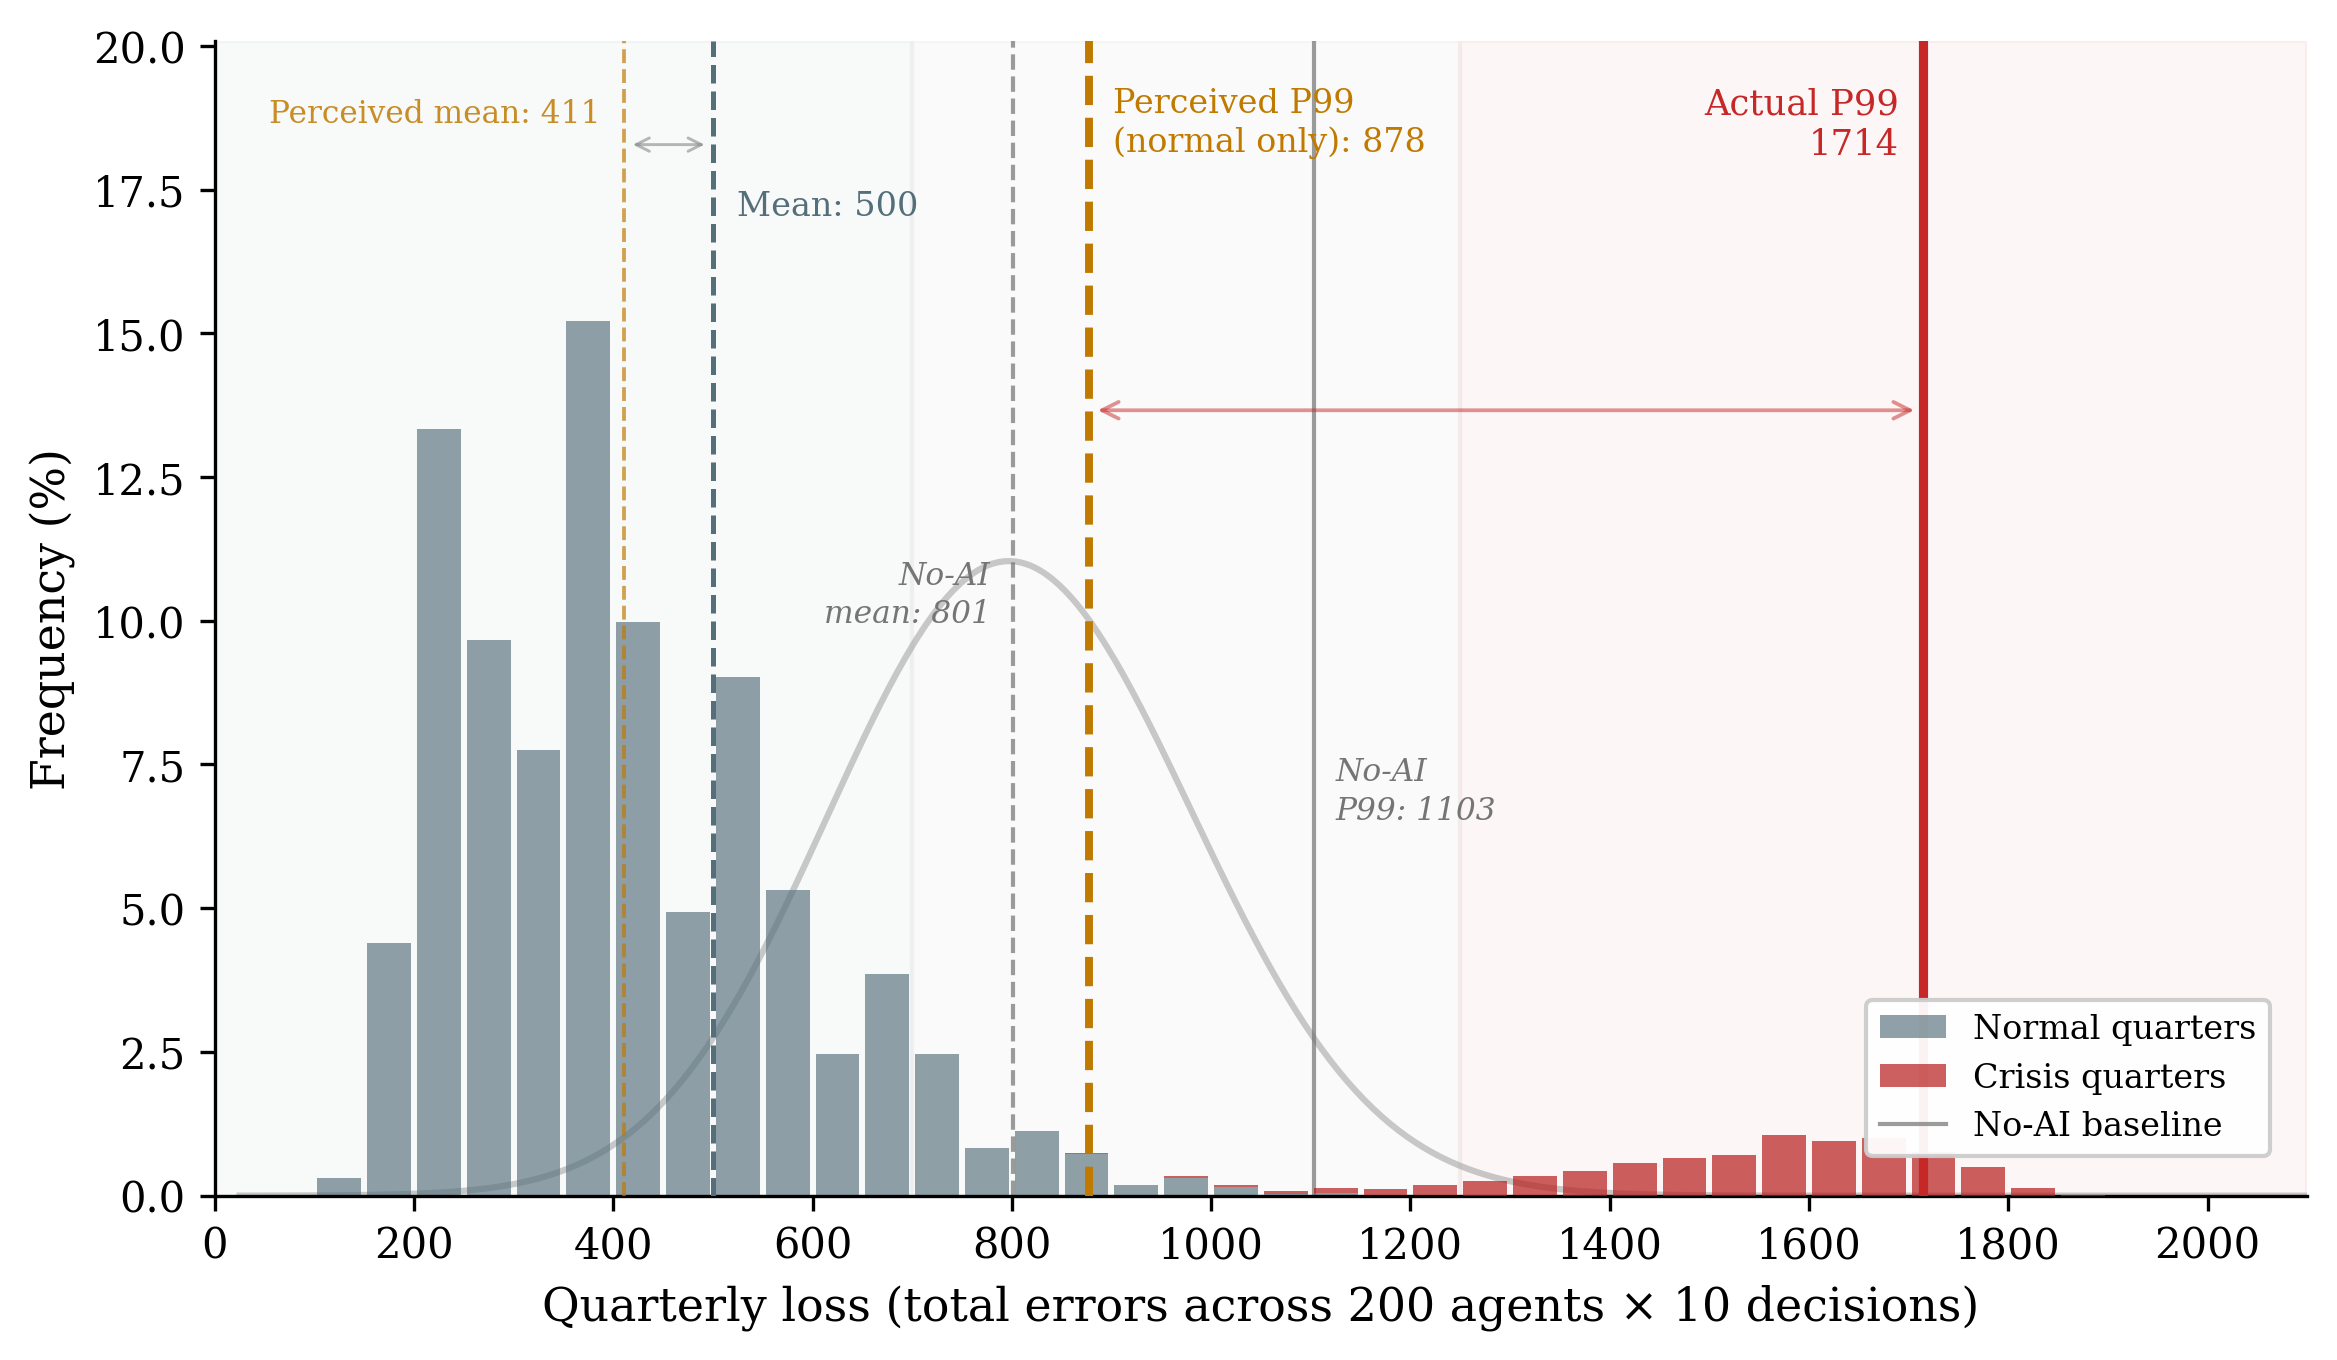
\includegraphics[width=0.85\textwidth,height=0.55\textheight,keepaspectratio]{../figures/exhibit1_essay.png}
  \caption{Bimodal distribution of quarterly losses under unmanaged AI
  adoption ($G_0$).
  Normal quarters (grey, 92\%) peak near 250;
  crisis quarters (red, 8\%) peak near 1{,}600.
  $E[L] = 500$ falls in the near-empty gap $[600, 1200]$.
  Perceived $P_{99}$ (normal quarters only) $= 878$;
  actual $P_{99} = 1{,}714$ (solid red line).
  Crisis regime couples $\pi_t$ with $\xi_t$ (Basel~II conditional stress).
  $\mu_{\text{crisis}}$, $\sigma_{\text{normal}}$, $\sigma_{\text{crisis}}$
  are calibrated stylisations.
  \textit{V5 coupled model, $M = 500$ replications, under model
  assumptions.}}
  \label{fig:bimodal}
\end{mdframed}
\end{figure}

Kahneman, Sibony, and Sunstein~\cite{kahneman_book_2021} document that human
decision-making in organisations is already characterised by enormous noise:
inter-rater variance reaching 55\% in insurance underwriting and spanning 5\%
to 88\% in asylum adjudication. The baseline noise they document is dispersed
across decision-makers rather than synchronised by a common signal. The
observation that this dispersion has a \textit{protective} property, that
unsynchronised noise generates error decorrelation, is our analytical
extension, not the authors' thesis. The 38\% reduction in expected loss that
AI adoption produces under $G_0$ is real. What the model shows is that
compressing dispersed variance into a synchronised mode eliminates that
protective property. Average-based metrics register the compression as a gain.

\subsection{The mean-tail paradox}

Under $G_0$ with the coupled $\pi$-$\xi$ model, the central case produces
the following metrics relative to the no-AI baseline:

\begin{table}[h!]
\centering
\small
\begin{tabular}{lrrl}
\toprule
\textbf{Metric} & \textbf{Baseline} & \textbf{G0} & \textbf{Change} \\
\midrule
$E[L]$ (expected quarterly loss) & 802 & 499 & $-38\%$ \\
$P_{99}$ brut & 1\,097 & 1\,708 & $+56\%$ \\
$P_{99}\times\theta$ (risk-adjusted) & 1\,097 & 2\,135 & $+94\%$ \\
Output (correct $\times\,\theta$) & 1\,198 & 1\,845 & $+54\%$ \\
Tail ratio $P_{99}/E[L]$ & 1.37 & 3.42 & $\times 2.5$ \\
\bottomrule
\end{tabular}
\caption{Mean-tail paradox under $G_0$. V5 coupled model, $M = 200$
replications, central case ($\alpha = 0.70$, $\mathrm{Beta}(2,2)$,
$E[\pi] = 0.70$). Under model assumptions.}
\label{tab:paradox}
\end{table}

Three channel dynamics reinforce each other over 20 quarters in the
calibrated model. $\text{Var}(\tau)$ falls by 30\% through screening.
Effective surrender rises from 69\% to 80\% through the H-channel. Mean
capability $\bar{h}$ decays from 0.60 to 0.50 through deskilling. Lower
diversity elevates conformism pressure via $\beta_{\text{conform}}$, which
amplifies surrender, which accelerates deskilling. The robustness of this
lock-in at low values of $\omega$ remains an active gap
(Section~\ref{sec:bridge}).
Figure~\ref{fig:correlation} tracks the build-up over 20 quarters.

\begin{figure}[H]
\begin{mdframed}[linewidth=0.5pt]
  \centering
  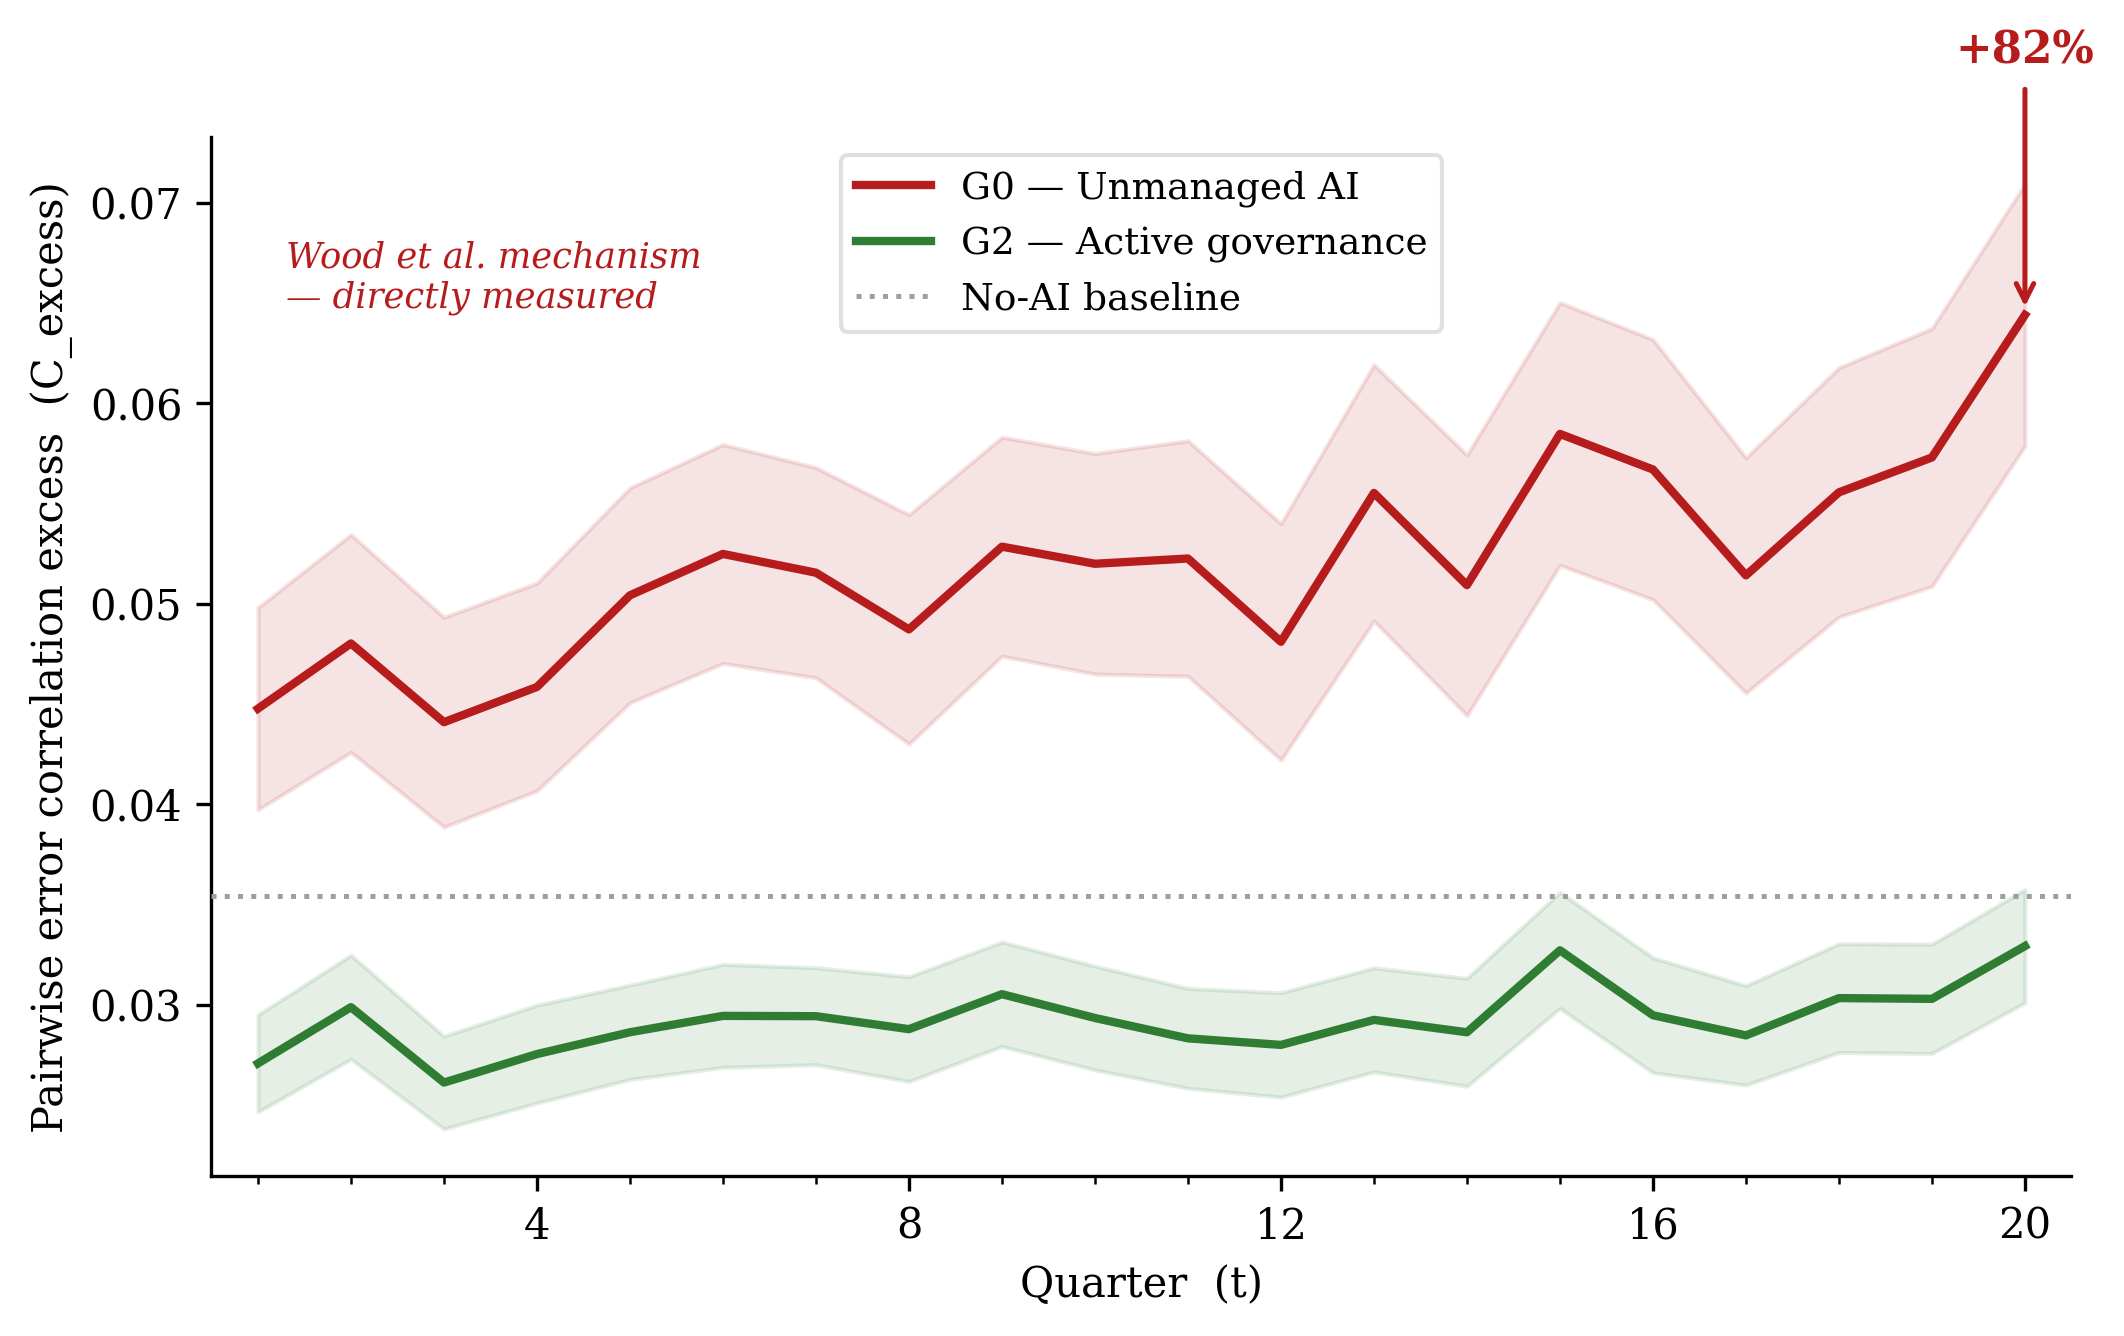
\includegraphics[width=0.85\textwidth]{../figures/exhibit4_essay.png}
  \caption{Pairwise error correlation excess
  ($\hat{C}_{\text{excess}}$) under $G_0$ (red) and $G_2$ (green) over
  20 quarters, with 95\% confidence intervals.
  Dotted line: no-AI baseline.
  Under $G_0$, correlation rises over five years, confirming the Wood et
  al.~\cite{wood_jmlr_2023} mechanism in simulation.
  Under $G_2$, correlation remains below the no-AI baseline throughout.
  \textit{V5 coupled model, $M = 200$ replications, under model
  assumptions.}}
  \label{fig:correlation}
\end{mdframed}
\end{figure}

The tail-to-mean ratio under $G_0$ is 3.42, compared to 1.37 at baseline.
That ratio is independent of $N$ (Section~\ref{sec:theory}). An
organisation of 20 people facing the same $\bar{\rho}$ and $\bar{p}$ as a
division of 5,000 produces the same relative tail exposure. What scales with
organisational size is the absolute loss absorbed, not the tail premium per
decision. This distinction matters in Section~\ref{sec:markets}: the risk
produced is size-independent; the risk that cannot be externalised is not.

\subsection{The masking mechanism and the top-tier twist}

Under $G_0$, AI adoption raises throughput by 54\%, the signal a standard
productivity dashboard reports. Over the same period,
$P_{99}\times\theta$ rises to $2{,}142$, a tail premium of 94\% above the
no-AI baseline. Both numbers are driven by the same multiplier applied to
different quantities. A signal informative about throughput is, under this
model, uninformative about tail dynamics.
Bainbridge~\cite{bainbridge_automatica_1983} observed that systems designed
to accelerate work render their own failure modes invisible; $\theta$
formalises that observation. The protective-noise interpretation is our
extension of Bainbridge, not a claim she makes.

The top-tier twist sharpens the masking. For organisations whose workforce
capability $\bar{h}$ substantially exceeds the outside-frontier threshold
$q_{\text{out}}$, the configuration corresponding to Paris consulting (P3)
under these parameters, the model produces $P_{99}\times\theta$ nearly 200\%
above baseline while apparent productivity rises by only 18\%. The masking is
most severe where talent is highest, because high-capability agents are
disproportionately exposed to outside-frontier tasks while still generating
strong apparent productivity gains. This result holds under
$\bar{h} \approx 0.80 > q_{\text{out}} = 0.55$. If the outside-frontier
threshold improves as AI systems develop, the twist attenuates.

Under governance, the tail premium contracts. $G_1$ (passive scaffold) leaves
it at approximately +40\% above baseline. $G_2$ (active scaffold) reduces it
to approximately +16\%~\cite{vaccaro_nhb_2024}. The throughput cost is real: $G_2$ reduces output from
+54\% to +26\% relative to baseline, a loss of 28 percentage points. That
trade-off, tail risk reduction purchased at the cost of throughput, is the
structural tension behind the argument in Section~\ref{sec:markets} that
competitive markets cannot sustain the efficient governance regime.
Figure~\ref{fig:frontier} maps the three regimes on the output--risk plane.

\begin{figure}[H]
\begin{mdframed}[linewidth=0.5pt]
  \centering
  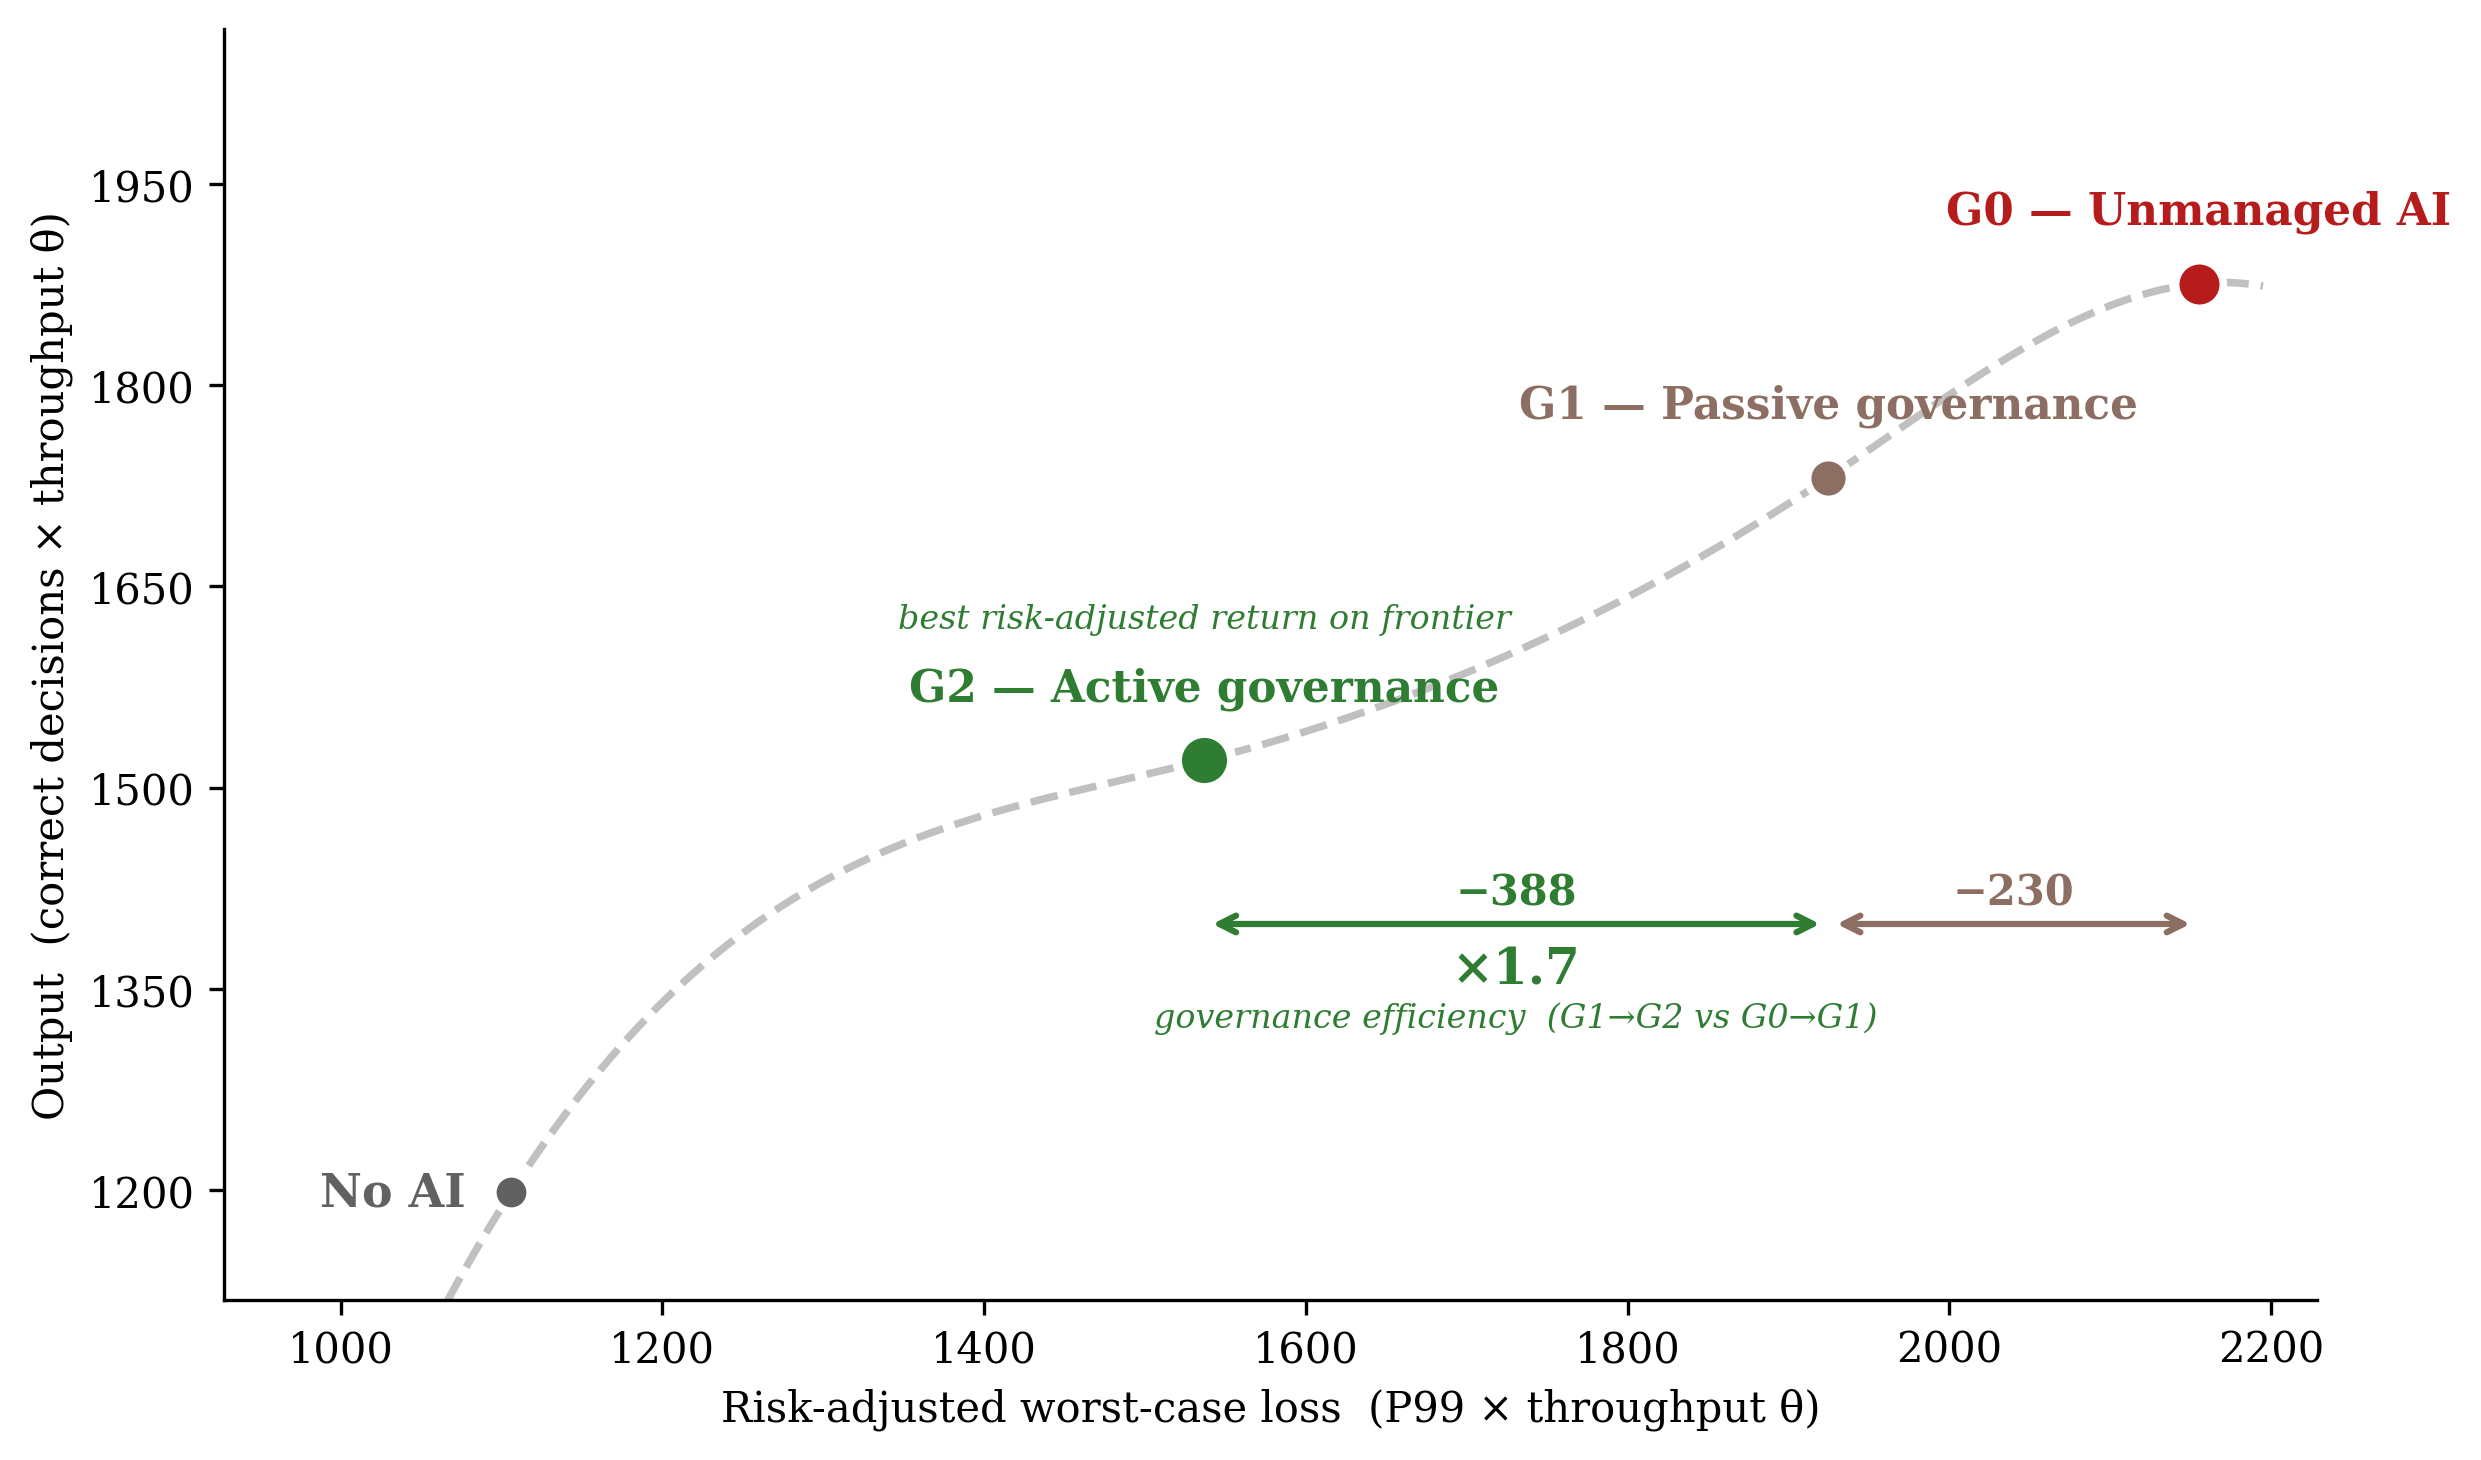
\includegraphics[width=0.85\textwidth]{../figures/exhibit2_essay.png}
  \caption{Risk-return frontier across governance regimes.
  Horizontal axis: output relative to no-AI baseline.
  Vertical axis: $P_{99}\times\theta$ (throughput-adjusted tail risk).
  $G_2$ sits at the elbow: the first gains in output (Baseline $\to G_2$)
  are purchased at low tail cost; the incremental gains ($G_2 \to G_0$)
  carry a 54\% output premium but a 94\% tail risk premium.
  The 28-percentage-point throughput cost of $G_2$ relative to $G_0$
  is the price of the elbow.
  \textit{V5 coupled model, $M = 200$ replications, under model assumptions.}}
  \label{fig:frontier}
\end{mdframed}
\end{figure}

\bridgeskip
\noindent\textit{These results describe the baseline case. The risk is not
uniformly distributed across organisations. Five structural parameters
determine position on the risk-return frontier, and their interaction
produces a spread that management decisions alone cannot close.}

$\alpha$ is the \textbf{within-organisation stack concentration parameter}.
It governs how strongly all agents in a single organisation respond to the
same systemic factor. The central value $\alpha = 0.70$ is a calibrated
stylisation, consistent with the synchronisation observed in the LTCM
convergence, the 2008 VaR monoculture, and the CrowdStrike 2024 failure. It
is not estimated econometrically. It is varied across $\{0.3, 0.5, 0.7,
1.0\}$ and is the dominant within-firm risk lever: reducing $\alpha$ from
0.90 to 0.30 cuts the tail risk premium by approximately 15\%
(Appendix~\ref{app:sensitivity}). In the v5 coupled model, the ratio
$P_{99}(\alpha{=}0.90)/P_{99}(\alpha{=}0.30)$ is approximately 1.15; the
crisis coupling $\mu_{\text{crisis}} = 2.2$ saturates crisis-quarter errors
across all $\alpha$ levels, compressing the marginal effect relative to
earlier model versions.

\section{Why markets cannot self-correct}\label{sec:markets}

\subsection{Two correlation channels, one regulatory implication}

The Vasicek parameter $\alpha$ governs within-organisation error
correlation, the primary risk driver documented in Section~\ref{sec:model}.
A second channel, $\kappa_{\text{vendor}}$, captures additional inter-firm
co-movement when multiple organisations share a common AI provider.
Simulation V6 estimates that this shared-vendor channel adds only 4\% of
marginal systemic correlation above the independent-vendor baseline.

These levers are not equivalent; the dominant contagion vector is
behavioural, not technical. What synchronises failures across firms is not
that they use the same vendor but that competitive pressure drives them all
toward the same governance regime. The monoculture that matters most is a
monoculture of unmanaged adoption.

Within-organisation stack concentration remains the primary variable:
reducing $\alpha$ from 0.90 to 0.30 cuts the tail risk premium by
approximately 15\% (Appendix~\ref{app:sensitivity}). The $G_2$ scaffold bundle
reduces tail risk by 19.2\% but is harder to mandate and verify externally,
because it requires coordinated changes to hiring, training, and workflow
design that are not directly observable to a
regulator. Peng and Garg~\cite{peng_neurips_2024} show that the governance
monoculture effect scales with the number of firms: as more organisations
converge on $G_0$, systemic tail risk grows faster than any individual
firm's exposure. This strengthens the case for mandatory standards.

The regulatory target that follows is the governance regime, not the vendor.
A regulator can require organisations above a certain scale to demonstrate a
floor on independent-judgement sequencing and a ceiling on AI-stack
concentration, in the same way Basel requires minimum capital ratios. That
target is more directly auditable than internal model choice, even if it
remains harder to observe than vendor concentration alone.

\subsection{The externalisation structure and the Nash equilibrium}

The tail-to-mean ratio is independent of $N$
(Section~\ref{sec:theory}). What scales with organisational size is the risk
absorbed: the fraction of the tail that falls inside the organisation rather
than being externalised through failure, employee attrition, or counterparty
loss.

For a startup with a five-year survival probability near 10\%, the expected
cost of the tail event is negligible relative to the 54\% productivity
advantage of $G_0$. The startup chooses $G_0$ rationally. P5 San Francisco
carries a governance efficiency of $-36\%$ under the calibrated
parameters. It does not marginally reject governance; it rejects it with a
large negative return. That is the correct calculation given the incentive
structure.

The competitive dynamics follow. Firms operating under $G_0$ outproduce
governed competitors by 54\%. Governed incumbents face pressure to reduce
governance friction or lose market share to less constrained entrants. The
Nash equilibrium without regulation is unmanaged adoption for all firms.
This argument is directional: it follows from the differential structure of
the simulation results, not from a calibrated market
model. Menlo Ventures~\cite{menlo_2025} estimates that approximately 88\%
of enterprise AI expenditure is concentrated among three providers (an
industry source cited for scale, not as a peer-reviewed finding). When most
firms depend on the same few systems, a governance-synchronised failure
propagates correlated losses at a scale no single firm's internal governance
can address.

\subsection{The financial precedent and its limits}

Danielsson and Shin~\cite{danielsson_endogenous_2012} describe the
Millennium Bridge failure as a model for financial systemic risk:
pedestrians adapted to bridge oscillations by synchronising their gait,
amplifying rather than damping the oscillations. Financial institutions
respond to shared risk signals in a structurally similar way, generating
collective fragility through individually rational decisions. Haldane and
May~\cite{haldane_nature_2011} documented that post-2008 reform moved
toward decorrelated architectural diversity in systemically important
institutions. Danielsson and Uthemann~\cite{danielsson_jfs_2025} warn that
AI adoption threatens to reverse this progress by reintroducing shared model
dependence at the workflow level. The claim that finance has learned from
2008 rests on practitioner observation rather than a direct peer-reviewed
source; it is noted here as context.

Bernile, Bhagwat, and Yonker~\cite{bernile_jfe_2018}, using instrumental
variable identification, show that board-level cognitive diversity reduces
firm-level return volatility and improves R\&D efficiency. This is one of
the few studies with causal identification on the diversity-to-risk
relationship at the organisational level. Citron and
Pasquale~\cite{citron_wlr_2014} documented the structural opacity of
automated scoring systems more than a decade before AI-assisted hiring
became widespread: the impossibility of contesting what cannot be observed
is a governance failure that predates the current
wave. Wright et al.~\cite{wright_facct_2024} find 4.6\% compliance with New
York City Local Law~144. EEOC guidelines were withdrawn in January~2025.
The EU AI Act, entering force in August~2026, contains no provisions
targeting AI-stack concentration.

\subsection{The Tragedy of the Cognitive Commons}

Each firm that maximises its AI productivity depletes the collective
resource on which systemic resilience depends: the diversity of cognitive
approaches across decision-makers in the economy. The conditions
Hardin~\cite{hardin_science_1968} identified as sufficient for a commons
tragedy are present: a shared resource, rational individual exploitation,
and no individual incentive to preserve. This is a proposed extension of
Hardin's framework, not an established result; it is named as such
throughout.

Two features distinguish this extension from the original pasture case.
The depletion is invisible, masked by $\theta$, and registers in no
standard dashboard. And it erodes the option of reversal. Organisations
that have operated under $G_0$ for several years cannot restore the
cognitive substrate governance requires by switching to $G_2$. Late
governance, adopted after 2.5 years of unmanaged adoption, still reduces
tail risk (Section~\ref{sec:results}, V4 verification: $-16.6\%$). But
it cannot restore the cognitive diversity already depleted: the gap between
early and late governance at year five represents a 6\% shortfall in
$\text{Var}(\tau)$ that the scaffold cannot recover. The window does not
close suddenly. It narrows continuously, and every quarter under unmanaged
adoption depletes the organisational capital that governance requires.

The lock-in is endogenous. The three channels (screening, conformism,
deskilling) are not only the mechanism through which tail risk builds; they
are also what stabilises the Nash equilibrium. As organisations homogenise
and deskill, the cost of transitioning from $G_0$ to $G_2$ rises. The
cognitive diversity the scaffold needs has already been depleted. The result
established in Section~\ref{sec:results}, that governance works least
where it is needed most, becomes systemic here.

\bridgeskip
\noindent\textit{Three structural assumptions bound the model's scope, and
none favours the conclusion.}

%% ================================================================
\section{Limitations and empirical agenda}\label{sec:limitations}

The preceding sections established a mechanism, encoded it in a simulation,
and traced its structural implications. This section identifies the points
where the argument is most fragile, names two model omissions whose
direction of error is known, and sets out what empirical work would sharpen
or refute the claim.

\subsection{Three structural limitations}

Each limitation below was anticipated in the relevant section and is
consolidated here for the reader assessing the argument as a whole.

\textbf{L1: The D$\rightarrow$H bridge is an inference.} The most fragile
juncture, as noted in Section~\ref{sec:bridge}, is the link between
cognitive profile compression and error decorrelation. Keck and
Tang~\cite{keck_psychsci_2020} show in laboratory conditions that
cognitively homogeneous groups produce strongly correlated errors. Our
argument requires that diversity of cognitive \textit{profiles}, the
quantity compressed by AI screening, serve as a reliable proxy for
diversity of cognitive \textit{processes} in organisational
decision-making. No published study has measured pairwise error correlations
before and after ATS deployment in a knowledge-work organisation. The
argument rests on the divergence of evaluation criteria, not on any claimed
superiority of atypical profiles. That is a more modest claim, but still an
inference.

\textbf{L2: The model is a stress test, not a forecast.} The simulation
omits external labour market dynamics, managerial adaptation over time,
sector-specific institutional constraints, and intra-organisational
heterogeneity in AI adoption intensity. It demonstrates that the mechanism
\textit{can} produce the paradox under plausible parameter combinations. It
does not predict that any specific organisation will reach the simulated
$P_{99}\times\theta$ values.

\textbf{L3: Social influence is not uniformly harmful.} Becker, Brackbill,
and Centola~\cite{becker_pnas_2017} show that decentralised social
influence improves collective accuracy when agents encounter diverse signals
from independent sources. Aggarwal et
al.~\cite{aggarwal_frontpsych_2019} find an inverted-U relationship between
cognitive diversity and collective intelligence ($\beta = -0.91$,
$t = -2.19$, $p = 0.03$): beyond an optimal level, excess diversity
degrades performance. The argument in this paper does not require that more
diversity is always better. It requires that AI adoption pushes
organisations \textit{below} the optimal threshold, not away from an already
excessive one. This claim has not been directly tested.

\subsection{Two model omissions that underestimate the risk}

Unlike typical model limitations, these are structural gaps whose direction
of error is known. Including them would increase the estimated tail risk
premium.

The first concerns inter-firm dynamics. Peng and
Garg~\cite{peng_neurips_2024} show that the governance monoculture effect
scales super-linearly with the number of firms: as adoption spreads,
systemic correlation grows faster than any individual firm's contribution.
The model treats each organisation in isolation. Extending it to a network
of firms interacting through shared labour markets, common training data,
and correlated failure modes would add a positive externality to the tail
risk that the current simulation does not capture.

The second concerns ascending selection.
Rivera~\cite{rivera_book_2015} documents that elite professional services
firms progressively select for cultural fit over time. Managers who survive
in AI-native organisations will disproportionately be those who have most
fully adopted AI-assisted workflows. The model's agent population is fixed;
it does not capture how the organisation's cognitive profile shifts as those
who maintain independent judgement leave or are not promoted. This omission
implies that the D-channel effects likely understate the long-run
compression of $\text{Var}(\tau)$.

\subsection{Empirical agenda in four levels}

The following is structured to be actionable, from what a research team
could accomplish in two years to what would require a decade.

\textbf{Minimal confirming evidence.} A field study correlating (a)~a
measure of cognitive diversity before and after AI-assisted ATS deployment
and (b)~a proxy for pairwise error correlation in subsequent decisions,
drawn from shared project outcomes, investment decisions, or audited
judgements. $N = 20$--$30$ organisations would suffice to test the
direction. This is the critical empirical gap. Brynjolfsson et
al.~\cite{brynjolfsson_stanford_2025}\,(!) provide a first sectoral signal:
their analysis finds a roughly 20\% decline in employment of developers
aged 22--25 relative to the 2022 peak, consistent with AI adoption
displacing entry-level talent and potentially compressing cognitive profile
diversity at the workforce entry point.

\textbf{Minimal disconfirming evidence.} Demonstrate that pairwise error
correlation does not increase materially in an organisation that has
compressed $\text{Var}(\tau)$ through AI screening. This would require
either that the Keck and Tang result does not generalise outside controlled
settings, or that $\beta_{\text{conform}}$ in real organisations is close to
zero. Both are testable.

\textbf{Near-term feasible tests.} Three designs require no new data
collection beyond what organisations already hold. First, network analysis
of shared decisions in internal communications (email threads, document
co-authorship, meeting participation) before and after AI adoption,
producing a computational proxy for judgement correlation. Second, a natural
experiment using organisations that temporarily suspended their AI-assisted
ATS between 2020 and 2024, providing pre- and post-suspension hiring
distribution data. Third, implementation of $C_{\text{excess}}$ as an
organisational KRI: monitoring pairwise error correlation across shared
decisions provides a leading indicator of tail risk accumulation that
average error rates cannot provide, as the bimodal distribution in
Section~\ref{sec:results} demonstrates.

\textbf{Full validation requirements.} Longitudinal measurement of $h_i(t)$
through standardised competence assessments, $\text{Var}(\tau)$ through
cognitive profiling at intake and annually, and $L(t)$ through tracked
decision outcomes, in a panel of organisations with variation in AI adoption
intensity and governance regime. The most tractable natural design:
organisations that adopted and then withdrew AI-assisted hiring between 2020
and 2024, where the withdrawal creates a discontinuity usable for
difference-in-differences estimation.

\subsection{Independent corroboration and scope}

Galesic et al.~\cite{galesic_pnas_2018} provide independent corroboration
of the core claim's direction: demographically diverse crowds are not
substantially more accurate on average, but they reduce the risk of extreme
collective failure~\cite{deoliveira_pnas_2018}. This is the reformulation the model supports: diversity
does not improve the mean decision; it protects against the tail event. The
finding arrives at that conclusion from a purely performance-based analysis.

Vallor~\cite{vallor_philtech_2015} extends the scope: automation delegation
erodes not only technical competence but the capacity for moral judgement.
If correct, the deskilling documented in Section~\ref{sec:surrender}
extends further than $\eta$ captures, reinforcing the direction of
underestimation noted above.

\bridgeskip
\noindent\textit{The mechanism is documented. The stress test quantifies it.
The empirical agenda identifies what would confirm or refute it. What
follows is the full technical specification.}

\clearpage
\begin{appendices}
\renewcommand{\thefigure}{A\arabic{figure}}
\setcounter{figure}{0}
\renewcommand{\thetable}{A\arabic{table}}
\setcounter{table}{0}

%% ================================================================
%% APPENDIX A — MODEL SPECIFICATION
%% ================================================================

\section{Model specification}\label{app:model}

\subsection{Overview}\label{app:model:overview}

The model places $N = 200$ agents in an organisation that adopts AI
assistance over $T = 20$ quarters. Each quarter, every agent makes $K = 10$
binary decisions. Two channels activate simultaneously: a screening channel
(D) that narrows the distribution of cognitive profiles through AI-assisted
hiring, and a surrender channel (H) that erodes independent judgement through
AI reliance and deskilling. The outcome variable is the quarterly aggregate
loss $L(t)$: the total number of erroneous decisions across all agents and
decisions in quarter~$t$. Standard runs use $M = 200$ replications per
scenario; the bimodal histogram (Exhibit~1) uses $M = 500$.

Four scenarios are compared: Baseline (no AI), $G_0$ (unmanaged adoption),
$G_1$ (passive scaffold), and $G_2$ (active scaffold). Eight organisational
archetypes vary the structural parameters across profiles P1--P8
(Appendix~\ref{app:calibration}). All results in the body use the v5 coupled
$\pi$-$\xi$ model described in \S\ref{app:model:regime}.

\subsection{Agent initialisation}\label{app:model:agents}

Each agent $i$ carries two state variables initialised at $t = 0$:

\textbf{Cognitive profile.}
$\tau_i \sim \mathrm{Beta}(2, 2)$ on $[0,1]$, unimodal, symmetric.
$\text{Var}_{\text{ref}} = 1/20 = 0.050$, used as the conformism reference
throughout.

\textbf{Capability.}
$h_i(0) \sim \mathrm{U}(0.4, 0.8)$: the probability that agent $i$ makes a
correct decision when exercising independent judgement.

\subsection{Temporal structure}\label{app:model:temporal}

At each quarter $t$, operations execute in the following order:

\begin{enumerate}[nosep, label=(\roman*)]
  \item \textbf{Environmental regime.}
    Draw $\pi_t$ from the mixture in \S\ref{app:model:regime}. This single
    draw governs all $K$ decisions.
  \item \textbf{Systemic factor.}
    Draw $\xi_t$ according to the regime coupling in \S\ref{app:model:regime}.
  \item \textbf{Turnover.}
    A fraction $\delta = 0.04$ of agents separates uniformly at random.
    Replacements are drawn from \S\ref{app:model:screening}.
  \item \textbf{Decisions.}
    Each agent makes $K = 10$ binary decisions (\S\ref{app:model:decisions}).
  \item \textbf{Deskilling.}
    Capabilities update (\S\ref{app:model:deskilling}).
\end{enumerate}

\subsection{The D-channel: screening and cognitive
diversity}\label{app:model:screening}

AI adoption follows a saturating exponential:
\[
  A_t = A_{\max}\bigl(1 - e^{-\kappa t}\bigr)
\]
With $A_{\max} = 0.80$ and $\kappa = 0.15$, adoption reaches approximately
0.53 by quarter~5 and 0.76 by quarter~20, approaching but not reaching the
ceiling within the simulation horizon. Note: this is a saturating
exponential, not a logistic. The body text (Section~\ref{sec:model}) should
be read accordingly.

Replacement hires are drawn from
$\mathrm{Beta}\bigl(2 + \gamma_{\text{eff}} A_t,\;
2 + \gamma_{\text{eff}} A_t\bigr)$. As $A_t$ rises, the distribution
concentrates. $\gamma_{\text{eff}}$ governs screening intensity:

\begin{table}[H]
\centering\small
\setlength{\tabcolsep}{8pt}
\renewcommand{\arraystretch}{1.20}
\begin{tabular}{@{}lcl@{}}
\toprule
\textbf{Scenario} & $\gamma_{\text{eff}}$ & \textbf{Rationale} \\
\midrule
$G_0$ (unmanaged)   & 5.0 & Proxy: Wilson \& Caliskan~\cite{wilson_aies_2024}, 85.1\% \\
$G_1$ (passive)     & 3.5 & Proxy: partial audit compliance~\cite{wright_facct_2024} \\
$G_2$ (active)      & 1.5 & Design: diversity-preserving target~\cite{mann_pnas_2017} \\
\bottomrule
\end{tabular}
\end{table}

Under $G_2$, 10\% of replacement hires are drawn from
$\mathrm{Beta}(2,2)$ regardless of $A_t$, providing a minimum diversity
reserve. Target under $G_0$: $\text{Var}(\tau_t)$ declines by approximately
30\% by $t = 20$.

\subsection{Environmental regime and Vasicek coupling
(v5)}\label{app:model:regime}

Each quarter, $\pi_t$ and $\xi_t$ are drawn jointly from a two-regime
mixture:
\[
(\pi_t,\,\xi_t) \;\sim\;
\begin{cases}
  \text{Normal (prob.\ } 1{-}p_{\text{crisis}}\text{):} &
    \pi_t \sim \mathrm{Beta}(a_n,b_n),\quad
    \xi_t \sim \mathcal{N}(0,\,\sigma_n^2) \\[6pt]
  \text{Crisis (prob.\ } p_{\text{crisis}}\text{):} &
    \pi_t \sim \mathrm{Beta}(a_c,b_c),\quad
    \xi_t \sim \mathcal{N}(\mu_{\text{crisis}},\,\sigma_c^2)
\end{cases}
\]

\textbf{Normal-regime Beta parameters.} Computed from the target mean
$E[\pi_{\text{normal}}]$ and concentration
$c_{\text{normal}} = 60$:\footnote{Renamed from
$\kappa_{\text{normal}}$ to avoid notation clash with the adoption rate
$\kappa$ in \S\ref{app:model:screening}.}
\[
  a_n = E[\pi_{\text{normal}}] \cdot c_{\text{normal}}, \qquad
  b_n = \bigl(1 - E[\pi_{\text{normal}}]\bigr) \cdot c_{\text{normal}}
\]
where
$E[\pi_{\text{normal}}]
  = \bigl(E[\pi] - p_{\text{crisis}} \cdot E[\pi_{\text{crisis}}]\bigr)
    \big/ (1 - p_{\text{crisis}})$.
For the central case ($E[\pi] = 0.70$):
$E[\pi_{\text{normal}}] = (0.70 - 0.08 \times 0.35)/0.92 = 0.730$,
giving $a_n = 43.8$, $b_n = 16.2$.

\textbf{Interpretation.}
$\pi_t$ is the fraction of quarter~$t$'s decisions falling inside the AI's
competence frontier. In normal quarters,
$E[\pi_{\text{normal}}] \approx 0.730$ (sd~$\approx 0.06$). In crisis
quarters, $E[\pi_{\text{crisis}}] = 0.35$: roughly 65\% of decisions fall
outside the frontier.

The systemic factor $\xi_t$ governs the correlation structure of AI errors
across decisions. In crisis quarters, $\xi_t$ is shifted
($\mu_{\text{crisis}} = 2.2$): AI errors become systematically correlated
when the training data is obsolete for all decisions simultaneously. This v5
coupling produces the bimodal loss distribution documented in
Section~\ref{sec:results}.

\textbf{Calibration status.}
$p_{\text{crisis}} = 0.08$ is anchored on Flyvbjerg et
al.~\cite{flyvbjerg_jmis_2022} (8--12\% major failure rate in large
IT-dependent projects).
$\mu_{\text{crisis}} = 2.2$, $\sigma_n = 0.25$, and $\sigma_c = 0.30$ are
calibrated stylisations set by grid search across approximately 30
combinations.
$\mu_{\text{crisis}}$ is conservative relative to the Basel~II stress
scenario ($\Phi^{-1}(0.999) = 3.09$).

\subsection{Decision process and error
structure}\label{app:model:decisions}

For each decision $k \in \{1, \ldots, K\}$ in quarter $t$:

\textbf{Step 1: Task type.}
Draw $\mathrm{type}_k \sim \mathrm{Bernoulli}(\pi_t)$.
If inside: $q_k = q_{\text{in}}(t) = 0.92 + 0.002\,t$.
If outside: $q_k = q_{\text{out}} = 0.55$.
Here $q_k$ is the marginal probability that the AI answers correctly on
decision~$k$.

\textbf{Step 2: AI error (Vasicek structure).}
Draw $\varepsilon_k \sim \mathcal{N}(0,1)$ independently. The AI errs on
decision $k$ if:
\[
  Z_{\text{AI},k}
  = \ind\!\Bigl[
      \sqrt{\alpha}\,\xi_t + \sqrt{1{-}\alpha}\,\varepsilon_k
      > \Phi^{-1}(q_k)
    \Bigr]
\]
The marginal probability of AI error is $P(Z_{\text{AI},k} = 1) = 1 - q_k$
when $\xi_t = 0$, preserving $q_k$ as unconditional AI accuracy. The
parameter $\alpha = 0.70$ governs within-quarter inter-decision correlation:
conditional on $\xi_t$, errors on decisions $k$ and $k'$ are correlated. A
high $\xi_t$ raises error probability across all $K$ decisions
simultaneously. All agents who follow the AI on decision $k$ receive the
same realisation $Z_{\text{AI},k}$.

\textbf{Step 3: Surrender.}
Agent $i$ follows the AI on decision $k$ with probability:
\[
  p_i^{\text{surr}}(t)
  = p_0^{\text{eff}}(t) - \beta_{\text{surr}}\,|\tau_i - \bar{\tau}(t)|
\]
where the conformism-adjusted baseline is:
\[
  p_0^{\text{eff}}(t)
  = \operatorname{clip}\!\left(
      p_0 \times \left[
        1 + \beta_{\text{conform}} \times
        \frac{\text{Var}_{\text{ref}} - \text{Var}(\tau_t)}
             {\text{Var}_{\text{ref}}}
      \right],\;0,\;0.98
    \right)
\]
When $\text{Var}(\tau_t) < \text{Var}_{\text{ref}}$, the organisation is
more homogeneous than the reference population: conformism pressure rises,
increasing the effective baseline surrender probability.

\textbf{Step 4: Outcome.}
Let $s_{ik}(t) \sim \mathrm{Bernoulli}\bigl(p_i^{\text{surr}}(t)\bigr)$.

\emph{If $s_{ik} = 1$ (follows AI):}
$\varepsilon_{ik} = Z_{\text{AI},k}$.

\emph{If $s_{ik} = 0$ (judges independently):}
Errors are drawn via a Gaussian copula over non-followers of decision~$k$,
with covariance $\Sigma_{ij} = \exp(-\lambda\,|\tau_i - \tau_j|)$,
$\lambda = 8.0$. Specifically: draw $u_k = Lz_k$ where $L$ is the Cholesky
factor of $\Sigma$ and $z_k \sim \mathcal{N}(0,I)$; then
$\varepsilon_{ik} = \ind\bigl[\Phi(u_{ik}) > h_i(t)\bigr]$.

Followers and non-followers of the same decision are assumed uncorrelated.
This is a simplifying assumption that could be relaxed in future work.

\medskip
\textbf{Three correlation levels are superposed:}
\begin{enumerate}[nosep, label=(\arabic*)]
  \item Perfect correlation among followers of the same AI decision~$k$.
  \item Partial inter-decision correlation for followers via the shared
        $\xi_t$ (governed by $\alpha$).
  \item Profile-distance-based correlation among independent judgers
        (governed by $\lambda$).
\end{enumerate}

\subsection{Deskilling}\label{app:model:deskilling}

\[
  h_i(t{+}1) = h_i(t)\bigl(1 - \eta_{\text{eff}}\,\bar{s}_i(t)\bigr)
\]
where $\bar{s}_i(t) = (1/K)\sum_k s_{ik}(t)$ is the fraction of decisions
in which agent~$i$ followed the AI. Deskilling is proportional to actual
surrender in that quarter; it does not occur in quarters where the agent
exercises independent judgement throughout. This is a conservative
simplification: diffuse deskilling through tool dependence alone is not
modelled.

\begin{table}[H]
\centering\small
\setlength{\tabcolsep}{8pt}
\renewcommand{\arraystretch}{1.20}
\begin{tabular}{@{}lcl@{}}
\toprule
\textbf{Scenario} & $\eta_{\text{eff}}$ & \textbf{Rationale} \\
\midrule
Baseline            & 0.000 & No AI exposure \\
$G_0$ (unmanaged)   & 0.020 & Proxy: Budzy\'{n} et al.~\cite{budzyn_lancetgh_2025}, $-6$pp \\
$G_1$ (passive)     & 0.015 & Interpolated \\
$G_2$ (active)      & 0.010 & Reduced surrender $\to$ reduced deskilling \\
\bottomrule
\end{tabular}
\end{table}

\textbf{Structural omission.}
Surrender probability does not depend on $h_i(t)$. The
deskilling$\to$surrender feedback loop is absent from the model.
Section~\ref{sec:surrender} names this as a source of underestimation of the
tail risk premium.

\subsection{Output metrics}\label{app:model:metrics}

\textbf{Raw quarterly loss:}
\[
  L(t) = \sum_{i=1}^{N}\sum_{k=1}^{K} \varepsilon_{ik}(t)
\]

\textbf{Throughput-adjusted loss:}
$L_\theta(t) = \theta_g \times L(t)$. The parameter $\theta$ scales
exposure volume: under faster throughput, the same correlated failure
propagates across more outputs before detection.

\begin{table}[H]
\centering\small
\setlength{\tabcolsep}{10pt}
\renewcommand{\arraystretch}{1.20}
\begin{tabular}{@{}lcccc@{}}
\toprule
& Baseline & $G_0$ & $G_1$ & $G_2$ \\
\midrule
$\theta_g$ & 1.00 & 1.25 & 1.20 & 1.10 \\
\bottomrule
\end{tabular}
\end{table}

\textbf{Correct-decision output:}
$\text{Output}(t) = \theta_g \times (NK - L(t))$.

\textbf{Excess pairwise error correlation (proposed KRI):}
\[
  \hat{C}_{\text{excess}}(t)
  = \frac{1}{|P|}\sum_{(i,j)\in P}
    \left[\frac{1}{K}\sum_k \varepsilon_{ik}\,\varepsilon_{jk}
          - f_i \times f_j\right]
\]
where $f_i = (1/K)\sum_k\varepsilon_{ik}$. This quantity is the proposed KRI
of Section~\ref{sec:limitations}: its monotonic rise under $G_0$ and
stability under $G_2$ constitute the direct simulation signature of the
Wood et al.~\cite{wood_jmlr_2023} mechanism.

\textbf{Summary statistics} across all $T \times M$ quarter-replications:
$E[L]$, $P_{99}[L(t)]$, $P_{99}[L_\theta(t)]$, tail ratio $P_{99}/E[L]$,
mean output.

\subsection{Analytical reference check}\label{app:model:refcheck}

The following calculations should be reproduced before running the full
simulation as a consistency check. All use the v5 AI error equation from
\S\ref{app:model:decisions}.

\bigskip
\textbf{Crisis quarter}
($\pi_t = 0.35$, $\xi_t = 2.2$, $\alpha = 0.70$, $G_0$,
$\mathrm{Beta}(2,2)$):

\begin{align*}
P(\text{AI errs} \mid \text{outside},\, \xi_t{=}2.2)
  &= \Phi\!\left(
       \frac{\sqrt{0.7}\times 2.2 - \Phi^{-1}(0.55)}{\sqrt{0.3}}
     \right)
  = \Phi(3.13) \approx 0.999 \\[6pt]
P(\text{AI errs} \mid \text{inside},\, \xi_t{=}2.2)
  &= \Phi\!\left(
       \frac{\sqrt{0.7}\times 2.2 - \Phi^{-1}(0.92)}{\sqrt{0.3}}
     \right)
  = \Phi(0.80) \approx 0.79
\end{align*}

Average AI error probability:
$0.65 \times 0.999 + 0.35 \times 0.79 \approx 0.926$.

Effective surrender rate ($\mathrm{Beta}(2,2)$,
$\beta_{\text{conform}}$ at $\text{Var}_{\text{ref}}$):
$\approx 0.69$.

Expected loss:
$200 \times 10 \times (0.69 \times 0.926 + 0.31 \times 0.40)
\approx 1{,}526$.

\smallskip
Implementation~A: 1,538 ($\pm 0.8\%$).
Implementation~B: 1,551 ($\pm 1.6\%$).
Both within tolerance.

\bigskip
\textbf{Normal quarter}
($\pi_t = 0.70$, $\xi_t = 0$):

\begin{align*}
P(\text{AI errs} \mid \text{outside},\, \xi_t{=}0)
  &= \Phi(-0.23) \approx 0.41 \\[6pt]
P(\text{AI errs} \mid \text{inside},\, \xi_t{=}0)
  &= \Phi(-2.57) \approx 0.005
\end{align*}

Average AI error probability:
$0.30 \times 0.41 + 0.70 \times 0.005 \approx 0.127$.

$E[L \mid \text{normal}] \approx 200 \times 10 \times
(0.69 \times 0.127 + 0.31 \times 0.40) \approx 424$.

\smallskip
Both implementations: $\approx 424$--$427$ ($\pm 1\%$).

\bigskip
\textbf{Baseline} (no AI):
$E[L] = 200 \times 10 \times 0.40 = 800$.
Simulation: $\approx 803$ ($\pm 0.4\%$).

\bigskip
\noindent\textit{Decision rule: if an implementation does not produce
$\approx 1{,}526$ (crisis) / $\approx 424$ (normal) / $\approx 800$
(baseline) for these three cases, there is a bug. Do not proceed to full
simulation runs.}

\begin{figure}[H]
\begin{mdframed}[linewidth=0.5pt]
  \centering
  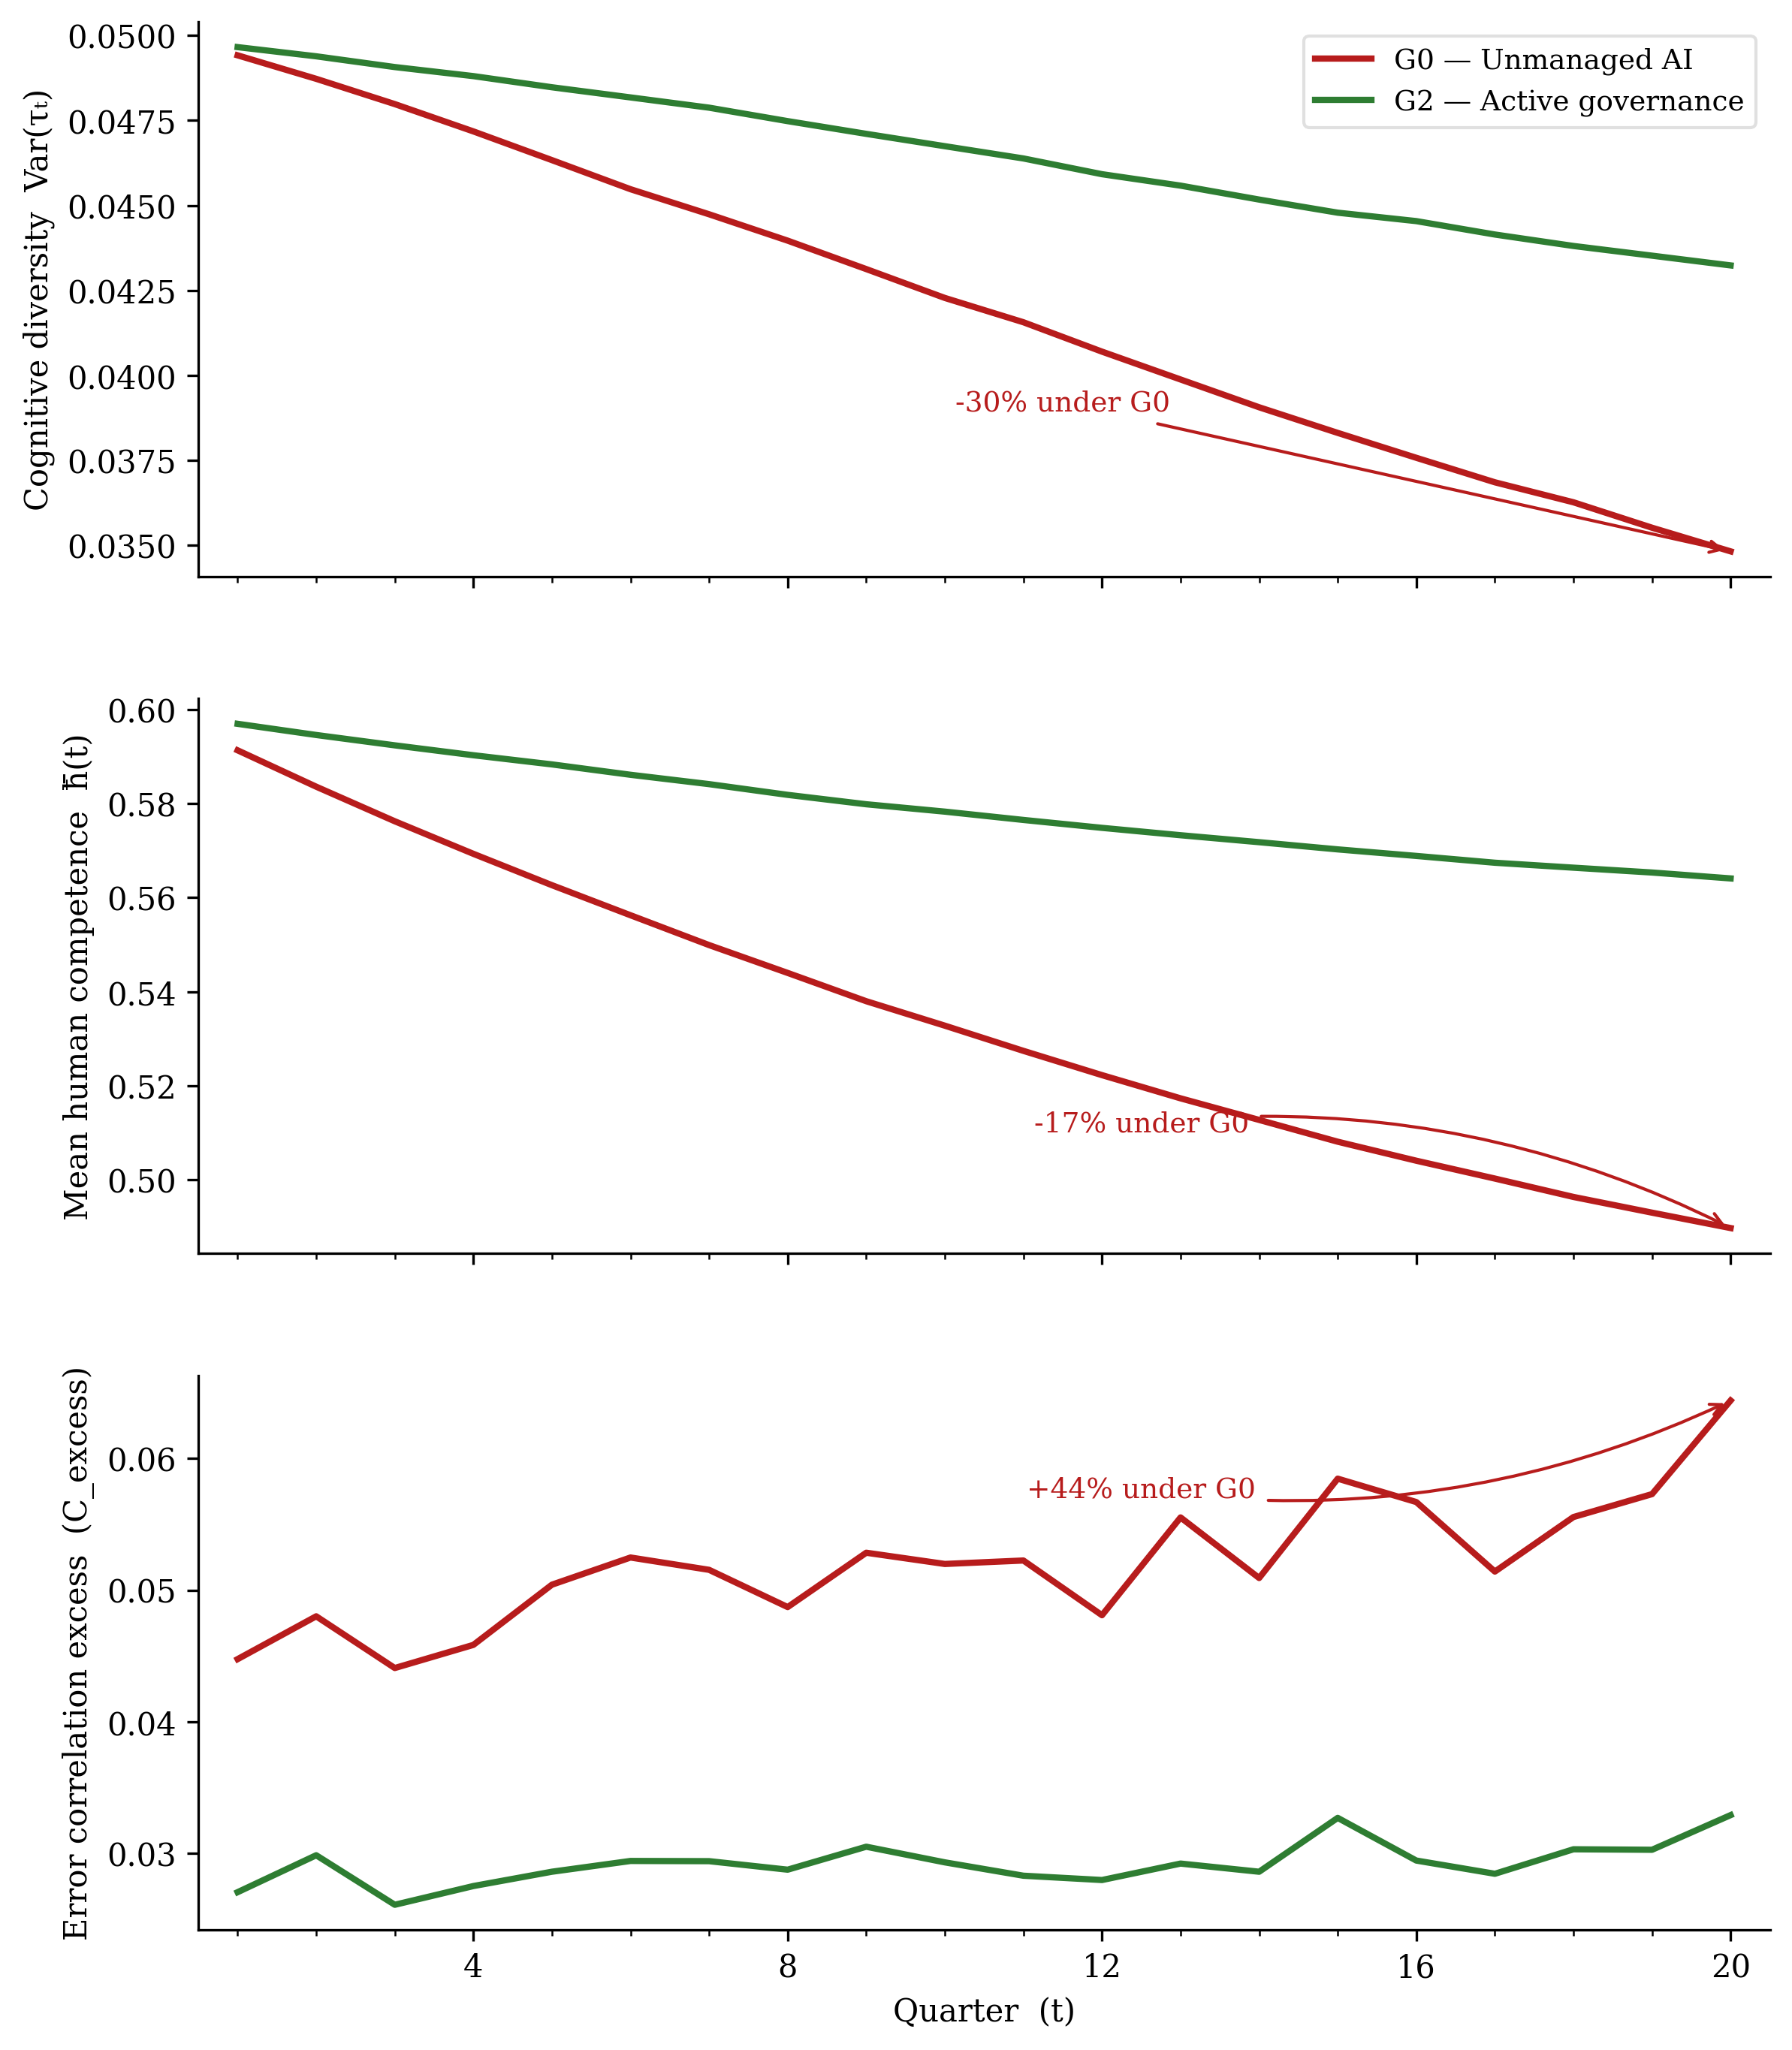
\includegraphics[width=0.85\textwidth]{../figures/fig_a1.png}
  \caption{Three channel dynamics under $G_0$ (red) and $G_2$ (green) over
  20 quarters.
  \textit{Top}: cognitive diversity $\text{Var}(\tau_t)$.
  \textit{Middle}: mean capability $\bar{h}(t)$.
  \textit{Bottom}: pairwise error correlation excess
  $\hat{C}_{\text{excess}}(t)$.
  Under $G_0$, diversity and capability decline monotonically while
  correlation rises. Under $G_2$, all three are preserved.
  \textit{V5 coupled model, under model assumptions.}}
  \label{fig:a1}
\end{mdframed}
\end{figure}


%% ================================================================
%% APPENDIX B — CALIBRATION TABLES
%% ================================================================

\section{Calibration tables}\label{app:calibration}

This appendix documents all 43 parameters\footnote{42 original parameters
plus $\omega$ (D$\rightarrow$H trajectory coupling), added in calibration
round~2.} of the v5 coupled model.
\S\ref{app:cal:main} reports the central-case values.
\S\ref{app:cal:profiles} lists profile-specific overrides for P1--P8.
\S\ref{app:cal:sensitivity} identifies the five most fragile parameters and
their sensitivity ranges.

For each parameter: symbol, description, central value, sensitivity range
(where varied), calibration method, epistemic status (one to five stars),
and primary source.

\subsection{Main parameter table}\label{app:cal:main}

\begin{landscape}
\footnotesize
\setlength{\tabcolsep}{4pt}
\renewcommand{\arraystretch}{1.25}
\begin{longtable}{
  >{\ttfamily}p{1.6cm}
  p{3.8cm}
  p{1.6cm}
  p{1.8cm}
  p{2.6cm}
  p{2.0cm}
  p{2.8cm}}
\toprule
\normalfont\textbf{Symbol} &
\textbf{Description} &
\textbf{Value} &
\textbf{Range} &
\textbf{Method} &
\textbf{Status} &
\textbf{Source} \\
\midrule
\endfirsthead
\multicolumn{7}{l}{\footnotesize\itshape continued from previous page} \\
\toprule
\normalfont\textbf{Symbol} &
\textbf{Description} &
\textbf{Value} &
\textbf{Range} &
\textbf{Method} &
\textbf{Status} &
\textbf{Source} \\
\midrule
\endhead
\midrule
\multicolumn{7}{r}{\footnotesize\itshape continued on next page} \\
\endfoot
\bottomrule
\endlastfoot

%% ── Structural ──
\multicolumn{7}{l}{\textit{Structural parameters}} \\
\midrule
N              & Number of agents          & 200              & ---
               & Architectural choice      & Stylisation
               & ---                                                       \\
T              & Horizon (quarters)        & 20               & ---
               & BLS tenure data           & Empirical
               & BLS JOLTS                                                 \\
K              & Decisions/agent/quarter   & 10               & ---
               & Architectural choice      & Stylisation
               & ---                                                       \\
M              & Replications              & 200              & 500 (Ex.~1)
               & Convergence test          & Stylisation
               & ---                                                       \\
$\delta$       & Quarterly separation rate & 0.04             & ---
               & BLS JOLTS (prof.\ services) & $\star\star\star\star\star$
               & BLS                                                       \\
\midrule

%% ── D-channel ──
\multicolumn{7}{l}{\textit{D-channel (screening)}} \\
\midrule
$A_{\max}$     & Adoption ceiling          & 0.80             & ---
               & SecondTalent/SHRM 2025    & Industry
               & SecondTalent                                              \\
$\kappa$       & Adoption growth rate      & 0.15             & ---
               & Exponential fit           & Stylisation
               & ---                                                       \\
$\gamma_{\text{eff}}$
               & Screening intensity ($G_0$) & 5.0            & \{1.5, 3.5, 5.0\}
               & Wilson \& Caliskan 85.1\% & Proxy~$\star\star\star\star$
               & \cite{wilson_aies_2024}                                   \\
\midrule

%% ── H-channel ──
\multicolumn{7}{l}{\textit{H-channel (surrender and deskilling)}} \\
\midrule
$p_0$          & Baseline surrender ($G_0$) & 0.80            & \{0.55, 0.70, 0.80\}
               & Shaw \& Nave 79.8\%       & Preprint~$\star\star\star\star$
               & \cite{shaw_psyarxiv_2026}                                 \\
$\beta_{\text{surr}}$
               & Surrender sensitivity     & 0.60             & \{0.4, 0.6, 0.8\}
               & Shaw \& Nave range        & Proxy~$\star\star\star$
               & \cite{shaw_psyarxiv_2026}                                 \\
$\beta_{\text{conform}}$
               & Conformism coefficient    & 0.30             & $[0.15, 0.35]$
               & Asch; Lorenz et al.       & Proxy~$\star\star\star$
               & \cite{asch_guetzkow_1951}                                 \\
$\text{Var}_{\text{ref}}$
               & Reference variance        & 0.050            & ---
               & $\mathrm{Beta}(2,2)$ exact & Exact
               & ---                                                       \\
$\lambda$      & Copula decay parameter    & 8.0              & ---
               & Keck \& Tang near-zero $\rho$ & Stylisation~$\star\star\star$
               & \cite{keck_psychsci_2020}\cite{kirton_routledge_2003}     \\
\midrule

%% ── AI quality ──
\multicolumn{7}{l}{\textit{AI quality}} \\
\midrule
$q_{\text{in}}(t)$
               & AI accuracy (inside)      & $0.92{+}0.002t$ & ---
               & Dell'Acqua +40\% quality  & $\star\star\star\star\star$
               & \cite{dellacqua_orgscience_2026}                          \\
$q_{\text{out}}$
               & AI accuracy (outside)     & 0.55             & ---
               & Dell'Acqua $-$19pp        & $\star\star\star\star\star$
               & \cite{dellacqua_orgscience_2026}\cite{magesh_jels_2025}   \\
\midrule

%% ── Environment ──
\multicolumn{7}{l}{\textit{Environment and correlation}} \\
\midrule
$E[\pi]$       & Inside-frontier fraction  & 0.70             & $[0.45, 0.85]$
               & Profile-specific          & Stylisation
               & ---                                                       \\
$\alpha$       & Stack concentration       & 0.70             & \{0.30, 0.50, 0.70, 1.00\}
               & Kim et al.\ 60\% inter-model & Indirect~$\star\star\star$
               & \cite{kim_icml_2025}\cite{wu_arxiv_2024}                  \\
$\eta$         & Deskilling rate (/quarter) & 0.02            & \{0.01, 0.02, 0.04\}
               & Budzy\'{n} et al.\ $-$6pp & Clinical proxy~$\star\star\star\star$
               & \cite{budzyn_lancetgh_2025}                               \\
\midrule

%% ── Crisis regime ──
\multicolumn{7}{l}{\textit{Crisis regime (v5 coupling)}} \\
\midrule
$p_{\text{crisis}}$
               & Crisis probability        & 0.08             & \{0.05, 0.08, 0.12\}
               & Flyvbjerg et al.\ 8--12\% & Anchor~$\star\star\star$
               & \cite{flyvbjerg_jmis_2022}                                \\
$\mu_{\text{crisis}}$
               & Crisis factor mean        & 2.2              & \{1.5, 2.0, 2.2, 2.5\}
               & Grid search ($<$Basel 3.09) & Stylisation~$\star\star$
               & ---                                                       \\
$\sigma_n$     & Normal-regime factor SD   & 0.25             & ---
               & Grid search               & Stylisation~$\star\star$
               & ---                                                       \\
$\sigma_c$     & Crisis-regime factor SD   & 0.30             & ---
               & Grid search               & Stylisation~$\star$
               & ---                                                       \\
$c_{\text{normal}}$
               & Normal Beta concentration & 60               & ---
               & Low-default analogy       & Stylisation
               & ---                                                       \\
$E[\pi_{\text{crisis}}]$
               & Outside fraction in crisis & 0.35            & ---
               & Dell'Acqua stress proxy   & Proxy~$\star\star\star\star$
               & \cite{dellacqua_orgscience_2026}                          \\
\midrule

%% ── Throughput ──
\multicolumn{7}{l}{\textit{Throughput}} \\
\midrule
$\theta_{G_0}$ & Throughput ($G_0$)        & 1.25             & ---
               & Dell'Acqua +25.1\% speed  & $\star\star\star\star\star$
               & \cite{dellacqua_orgscience_2026}                          \\
$\theta_{G_1}$ & Throughput ($G_1$)        & 1.20             & ---
               & Interpolated              & Stylisation
               & ---                                                       \\
$\theta_{G_2}$ & Throughput ($G_2$)        & 1.10             & ---
               & Governance cost estimate  & Stylisation
               & ---                                                       \\
\midrule

%% ── Inter-firm and coupling ──
\multicolumn{7}{l}{\textit{Inter-firm and trajectory coupling}} \\
\midrule
$\kappa_{\text{vendor}}$
               & Vendor correlation        & $+4\%$           & ---
               & V6 simulation             & Output
               & ---                                                       \\
$\omega$       & D$\to$H coupling          & 0.05             & \{0.02, 0.05, 0.10\}
               & Grid search               & Active gap~$\star$
               & ---                                                       \\
\end{longtable}
\end{landscape}


\subsection{Profile-specific overrides
(P1--P8)}\label{app:cal:profiles}

The values below override the central parameters from \S\ref{app:cal:main}
for each archetype simulation. Where no override is marked, the central
value applies. City labels are shorthand for documented labour market
structures, not predictions about specific organisations.

\smallskip
$\dag$~= override from central value. \quad
$\ast$~= expertise-gradient override ($p_0$ reduced for top-tier profiles
following Dratsch et al.~\cite{dratsch_radiol_2023}).

\begin{table}[H]
\centering\footnotesize
\setlength{\tabcolsep}{5pt}
\renewcommand{\arraystretch}{1.35}
\begin{tabular}{@{}l r r r r r r l@{}}
\toprule
\textbf{Profile} &
$E[\pi]$ &
$\alpha$ &
\textbf{Beta}$(a,a)$ &
$p_0^{G_0}$ &
$p_0^{G_2}$ &
$\eta$ &
\textbf{Source} \\
\midrule
P1 Frankfurt (Big Four)
  & 0.50 & 0.70$\dag$ & 3.5 & 0.75$\ast$ & 0.50 & 0.02
  & \cite{rivera_asr_2012} \\
P2 London (Inv.\ bank)
  & 0.55 & 0.45$\dag$ & 1.5$\dag$ & 0.70$\ast$ & 0.42 & 0.02
  & \cite{rivera_book_2015} \\
P3 Paris (Strategy)
  & 0.55 & 0.90$\dag$ & 4.0$\dag$ & 0.70$\ast$ & 0.42 & 0.02
  & \cite{bonneau_ipp_2021}\cite{bourdieu_noblesse_1989} \\
P4 Brussels (Legal)
  & 0.45$\dag$ & 0.90$\dag$ & 3.0$\dag$ & 0.80 & 0.55 & 0.01$\dag$
  & \cite{dahl_jla_2024} \\
P5 SF (Startup)
  & 0.70 & 0.60$\dag$ & 2.5$\dag$ & 0.80 & 0.70 & 0.03$\dag$
  & \cite{menlo_2025} \\
P6 Singapore (Creative)
  & 0.85$\dag$ & 0.30$\dag$ & 1.5$\dag$ & 0.80 & 0.55 & 0.01$\dag$
  & \cite{schneider_pp_1987} \\
P7 Bangalore (Back-office)
  & 0.75$\dag$ & 0.70 & 2.0$\dag$ & 0.85$\dag$ & 0.78 & 0.04$\dag$
  & \cite{oh_jorgbeh_2018}\cite{damato_emr_2021}\cite{schneider_jap_1998} \\
P8 Seoul (Central admin.)
  & 0.60 & 0.95$\dag$ & 4.5$\dag$ & 0.80 & 0.55 & 0.01$\dag$
  & \cite{oh_jorgbeh_2018} \\
\bottomrule
\end{tabular}
\caption{Profile-specific parameter overrides. All other parameters take
central values from \S\ref{app:cal:main}. $E[\pi]$ is the inside-frontier
fraction: $E[\pi] = 0.85$ means 85\% of decisions fall inside the AI's
competence frontier.}
\label{tab:profile_params}
\end{table}


\subsection{Five fragile parameters}\label{app:cal:sensitivity}

The following parameters have the largest impact on $P_{99}$ and the weakest
empirical anchoring. Sensitivity analysis (Appendix~\ref{app:sensitivity})
varies each across its stated range.

\medskip
\textbf{$\alpha$ (stack concentration).}
$\{0.30, 0.50, 0.70, 1.00\}$. Dominant lever. Reducing from $\alpha = 0.90$
to $\alpha = 0.30$ cuts the tail risk premium by approximately 15\%. In the
v5 coupled model, the ratio
$P_{99}(\alpha{=}0.90)\,/\,P_{99}(\alpha{=}0.30) \approx 1.15$: the crisis
coupling ($\mu_{\text{crisis}} = 2.2$) saturates crisis-quarter errors across
all $\alpha$ levels, compressing the marginal effect relative to earlier
model versions. Ablation result, not econometric estimate.

\medskip
\textbf{$p_{\text{crisis}}$ (crisis frequency).}
$\{0.05, 0.08, 0.12\}$. Second most sensitive parameter after $\alpha$.
Direction of the paradox is robust across the full range; magnitude varies.

\medskip
\textbf{$\mu_{\text{crisis}}$ (crisis severity).}
$\{1.50, 2.00, 2.20, 2.50\}$. Set by grid search across approximately 30
combinations. Conservative relative to Basel~II stress scenario
($\Phi^{-1}(0.999) = 3.09$).

\medskip
\textbf{$\beta_{\text{conform}}$ (conformism).}
$[0.15, 0.35]$. Maximum $\pm 1.5\%$ deviation in $P_{99}$ within this
range. ``Non-critical'' refers to low impact on the tail metric, not to the
theoretical importance of the conformism mechanism.

\medskip
\textbf{$\omega$ (D$\rightarrow$H trajectory coupling).}
$\{0.02, 0.05, 0.10\}$. Active gap. Direction is robust: lower diversity
raises conformism pressure via $\beta_{\text{conform}}$ regardless of
$\omega$. Magnitude is uncertain. See Section~\ref{sec:bridge}.

\section{Sensitivity analysis}\label{app:sensitivity}

This appendix reports single-parameter sensitivity for the five parameters
with the largest effect on model results: $\alpha$ (stack concentration),
$\mu_{\text{crisis}}$ (crisis severity), $\eta$ (deskilling rate),
$p_{\text{crisis}}$ (crisis frequency), and $\beta_{\text{conform}}$
(conformism coefficient). A sixth parameter, $\omega$ (D$\rightarrow$H
trajectory coupling), is treated separately in \S\ref{app:sens:omega} as an
exploratory extension. Each of the five main parameters is varied across
three levels while all others are held at central values.

Two questions are addressed: (1)~whether the direction of the mean-tail
paradox holds across the full tested range, and (2)~how much the magnitude
of the tail risk premium varies. The outcome metric throughout is
$P_{99}\times\theta$ under $G_0$. Figure~\ref{fig:a2} displays the tornado
chart.

\subsection{Sensitivity summary}\label{app:sens:summary}

Table~\ref{tab:sensitivity} reports $P_{99}\times\theta$ ($G_0$) at the
low, central, and high level of each parameter. The $\Delta$ column gives
the absolute and relative spread. The $\beta_{\text{conform}}$ range is
formally tested over $[0.15, 0.35]$, the anchored range from
Appendix~\ref{app:calibration}. An exploratory extension to 0.40 changes
$P_{99}\times\theta$ by at most 6 additional points and is not included.

\begin{table}[H]
\centering\small
\setlength{\tabcolsep}{8pt}
\renewcommand{\arraystretch}{1.20}
\begin{tabular}{@{}l r r r r@{}}
\toprule
\textbf{Parameter} &
\textbf{Low} & \textbf{Central} & \textbf{High} &
\textbf{$\Delta$ range} \\
\midrule
$\alpha$ (stack conc.)
  & 1{,}909 & 2{,}135 & 2{,}229 & 319~pts (15\%) \\
$\mu_{\text{crisis}}$ (severity)
  & 2{,}016 & 2{,}135 & 2{,}178 & 162~pts (8\%) \\
$\eta$ (deskilling)
  & 2{,}122 & 2{,}135 & 2{,}180 & 58~pts (3\%) \\
$p_{\text{crisis}}$ (frequency)
  & 2{,}114 & 2{,}135 & 2{,}170 & 56~pts (3\%) \\
$\beta_{\text{conform}}$ (conformism)
  & 2{,}111 & 2{,}135 & 2{,}141 & 30~pts (1.4\%) \\
\bottomrule
\end{tabular}
\caption{$P_{99}\times\theta$ ($G_0$) at low, central, and high parameter
levels. V5 coupled model, $M = 200$ replications, $\pm 2\%$ convergence
confirmed. Tornado chart: Figure~\ref{fig:a2}.}
\label{tab:sensitivity}
\end{table}

\subsection{Robustness of the mean-tail paradox}\label{app:sens:robustness}

The central claim, that AI adoption simultaneously reduces expected loss and
increases tail risk, holds at every tested parameter level.
Table~\ref{tab:robustness} reports the mean-tail split for each variation.
The paradox does not reverse under any tested combination. What varies is
the magnitude: the $P_{99}$ increase above baseline ranges from +39\% (at
$\alpha = 0.30$) to +61\% (at $\alpha = 1.00$), with the central estimate
at +56\%.

\begin{table}[H]
\centering\small
\setlength{\tabcolsep}{8pt}
\renewcommand{\arraystretch}{1.20}
\begin{tabular}{@{}l r r c@{}}
\toprule
\textbf{Parameter level} &
\textbf{$E[L]$ vs baseline} &
\textbf{$P_{99}$ vs baseline} &
\textbf{Paradox?} \\
\midrule
$\alpha = 0.30$ (low)           & $-35\%$ & $+39\%$ & Yes \\
$\alpha = 0.70$ (central)       & $-38\%$ & $+56\%$ & Yes \\
$\alpha = 1.00$ (high)          & $-40\%$ & $+61\%$ & Yes \\
\addlinespace
$\mu_{\text{crisis}} = 1.50$    & $-39\%$ & $+45\%$ & Yes \\
$\mu_{\text{crisis}} = 2.50$    & $-37\%$ & $+57\%$ & Yes \\
\addlinespace
$p_{\text{crisis}} = 0.05$      & $-41\%$ & $+54\%$ & Yes \\
$p_{\text{crisis}} = 0.12$      & $-33\%$ & $+58\%$ & Yes \\
\addlinespace
$\eta = 0.01$ (low)             & $-37\%$ & $+54\%$ & Yes \\
$\eta = 0.04$ (high)            & $-38\%$ & $+57\%$ & Yes \\
\addlinespace
$\beta_{\text{conform}} = 0.15$ & $-38\%$ & $+55\%$ & Yes \\
$\beta_{\text{conform}} = 0.35$ & $-38\%$ & $+56\%$ & Yes \\
\bottomrule
\end{tabular}
\caption{Mean-tail split across all parameter variations. Changes are
relative to no-AI baseline ($P_{99}$ brut, not throughput-adjusted). V5
coupled model, $M = 200$ replications.}
\label{tab:robustness}
\end{table}

\subsection{Parameter-level discussion}\label{app:sens:narrative}

\textbf{$\alpha$ (stack concentration).}
Dominant lever, approximately 2:1 over the next parameter. Reducing $\alpha$
from 0.70 to 0.30 reduces $P_{99}\times\theta$ from 2,135 to 1,909 and
the $P_{99}$ brut premium from +56\% to +39\% above baseline. At
$\alpha = 1.00$, $P_{99}\times\theta$ reaches 2,229.

This dominance makes stack concentration a natural regulatory target.
Whether that target is operationalisable as a mandated standard depends on
how governance frameworks define and audit internal AI workflow
architecture, a question beyond the model's scope.

\textbf{$\mu_{\text{crisis}}$ (crisis severity).}
Second most sensitive parameter (range 162~points). The central value 2.2 is
conservative relative to the Basel~II stress scenario
($\Phi^{-1}(0.999) = 3.09$). At $\mu_{\text{crisis}} = 1.50$,
$P_{99}\times\theta$ falls to 2,016 (+45\% premium). At 2.50 it reaches
2,178. This parameter governs how severely the AI is miscalibrated when the
environment shifts. It is a calibrated stylisation; the sensitivity range is
reported precisely because the central value lacks direct empirical
grounding.

\textbf{$p_{\text{crisis}}$ (crisis frequency).}
Produces an asymmetric pattern. As crisis frequency rises from 0.05 to
0.12, the mean gain from AI adoption shrinks ($-41\%$ to $-33\%$ on
$E[L]$) while the tail premium grows (+54\% to +58\%). More crisis quarters
means more quarters where the AI is unreliable, eroding the average benefit
while amplifying the tail. The central calibration $p_{\text{crisis}} =
0.08$ may be conservative for sectors facing more frequent structural shocks
than the IT project base rate anchoring it~\cite{flyvbjerg_jmis_2022}.

\textbf{$\eta$ (deskilling rate).}
Small direct effect on $P_{99}\times\theta$ in the single-parameter
protocol (58~points, $\sim$3\%), because deskilling accumulates slowly
relative to the crisis-driven tail. Its importance is primarily
longitudinal: over 20 quarters, $\bar{h}$ declines by 17.2\% under $G_0$
(from 0.591 to 0.490), the deskilling result underpinning the
irreversibility argument of Section~\ref{sec:markets}. The sensitivity range
spans the proxy transfer from clinical
medicine~\cite{budzyn_lancetgh_2025,kahol_jse_2010} to knowledge work. Direction is robust
throughout.

\textbf{$\beta_{\text{conform}}$ (conformism).}
Non-critical within the tested range $[0.15, 0.35]$:
$P_{99}\times\theta$ varies from 2,111 to 2,141, a spread under 1.5\%.
$\beta_{\text{conform}}$ is theoretically important as the formal expression
of the D$\rightarrow$H coupling, but its magnitude does not drive the
quantitative results within the anchored range.

\subsection{Exploratory extension:
$\omega$}\label{app:sens:omega}

The parameter $\omega$ is not part of the final calibrated model. In
Appendix~\ref{app:model}, the D$\rightarrow$H coupling is carried entirely
by $\beta_{\text{conform}}$: as $\text{Var}(\tau)$ falls, the conformism
mechanism raises $p_0^{\text{eff}}$, amplifying surrender. $\omega$
represents a second, direct coupling pathway: the possibility that diversity
compression raises surrender rates through channels not captured by
$\beta_{\text{conform}}$ alone (accelerated information cascades, reduced
access to dissenting colleagues).

$\omega$ is explored as a sensitivity extension rather than a calibrated
parameter because no direct empirical estimate exists. Preliminary grid
search over $\{0.02, 0.05, 0.10\}$ as an additive amplifier to the
$\beta_{\text{conform}}$ pathway produces $P_{99}\times\theta$ ($G_0$)
ranging from approximately 2,100 to 2,220, a spread comparable to the
$\mu_{\text{crisis}}$ sensitivity. The direction of the paradox holds
throughout.

The absence of $\omega$ from the final model is a structural omission whose
direction is known: including it would increase the estimated tail risk
premium, not reduce it. Section~\ref{sec:limitations} identifies measuring
the direct D$\rightarrow$H coupling as the primary empirical priority.

\subsection{Note on parameter
interactions}\label{app:sens:interactions}

All tests in
\S\ref{app:sens:summary}--\S\ref{app:sens:narrative} are single-parameter
variations. The model contains at least two interaction effects not captured
by this protocol.

First, $\alpha$ and $\beta_{\text{conform}}$ interact multiplicatively. A
homogeneous organisation (amplified $\beta_{\text{conform}}$ effect) that
also uses a centralised AI workflow (high $\alpha$) faces compound
amplification exceeding the sum of individual effects. This interaction is
the structural source of the Paris--London contrast in
Section~\ref{sec:results}.

Second, $p_{\text{crisis}}$ and $\mu_{\text{crisis}}$ jointly determine
crisis severity. Holding one fixed while varying the other understates the
joint tail exposure. A grid search over
$(p_{\text{crisis}}, \mu_{\text{crisis}})$ pairs is on the empirical agenda.

\medskip
\noindent\textit{Conclusion.} Across all tested single-parameter variations,
the mean-tail paradox holds without exception. $P_{99}\times\theta$ ($G_0$)
ranges from +39\% to +61\% above baseline, with +56\% as the central
estimate. $\alpha$ is the dominant lever. $\beta_{\text{conform}}$ is the
least quantitatively sensitive parameter within its anchored range. $\omega$
remains outside the calibrated model; its inclusion would increase the tail
risk premium.

\begin{figure}[H]
\begin{mdframed}[linewidth=0.5pt]
  \centering
  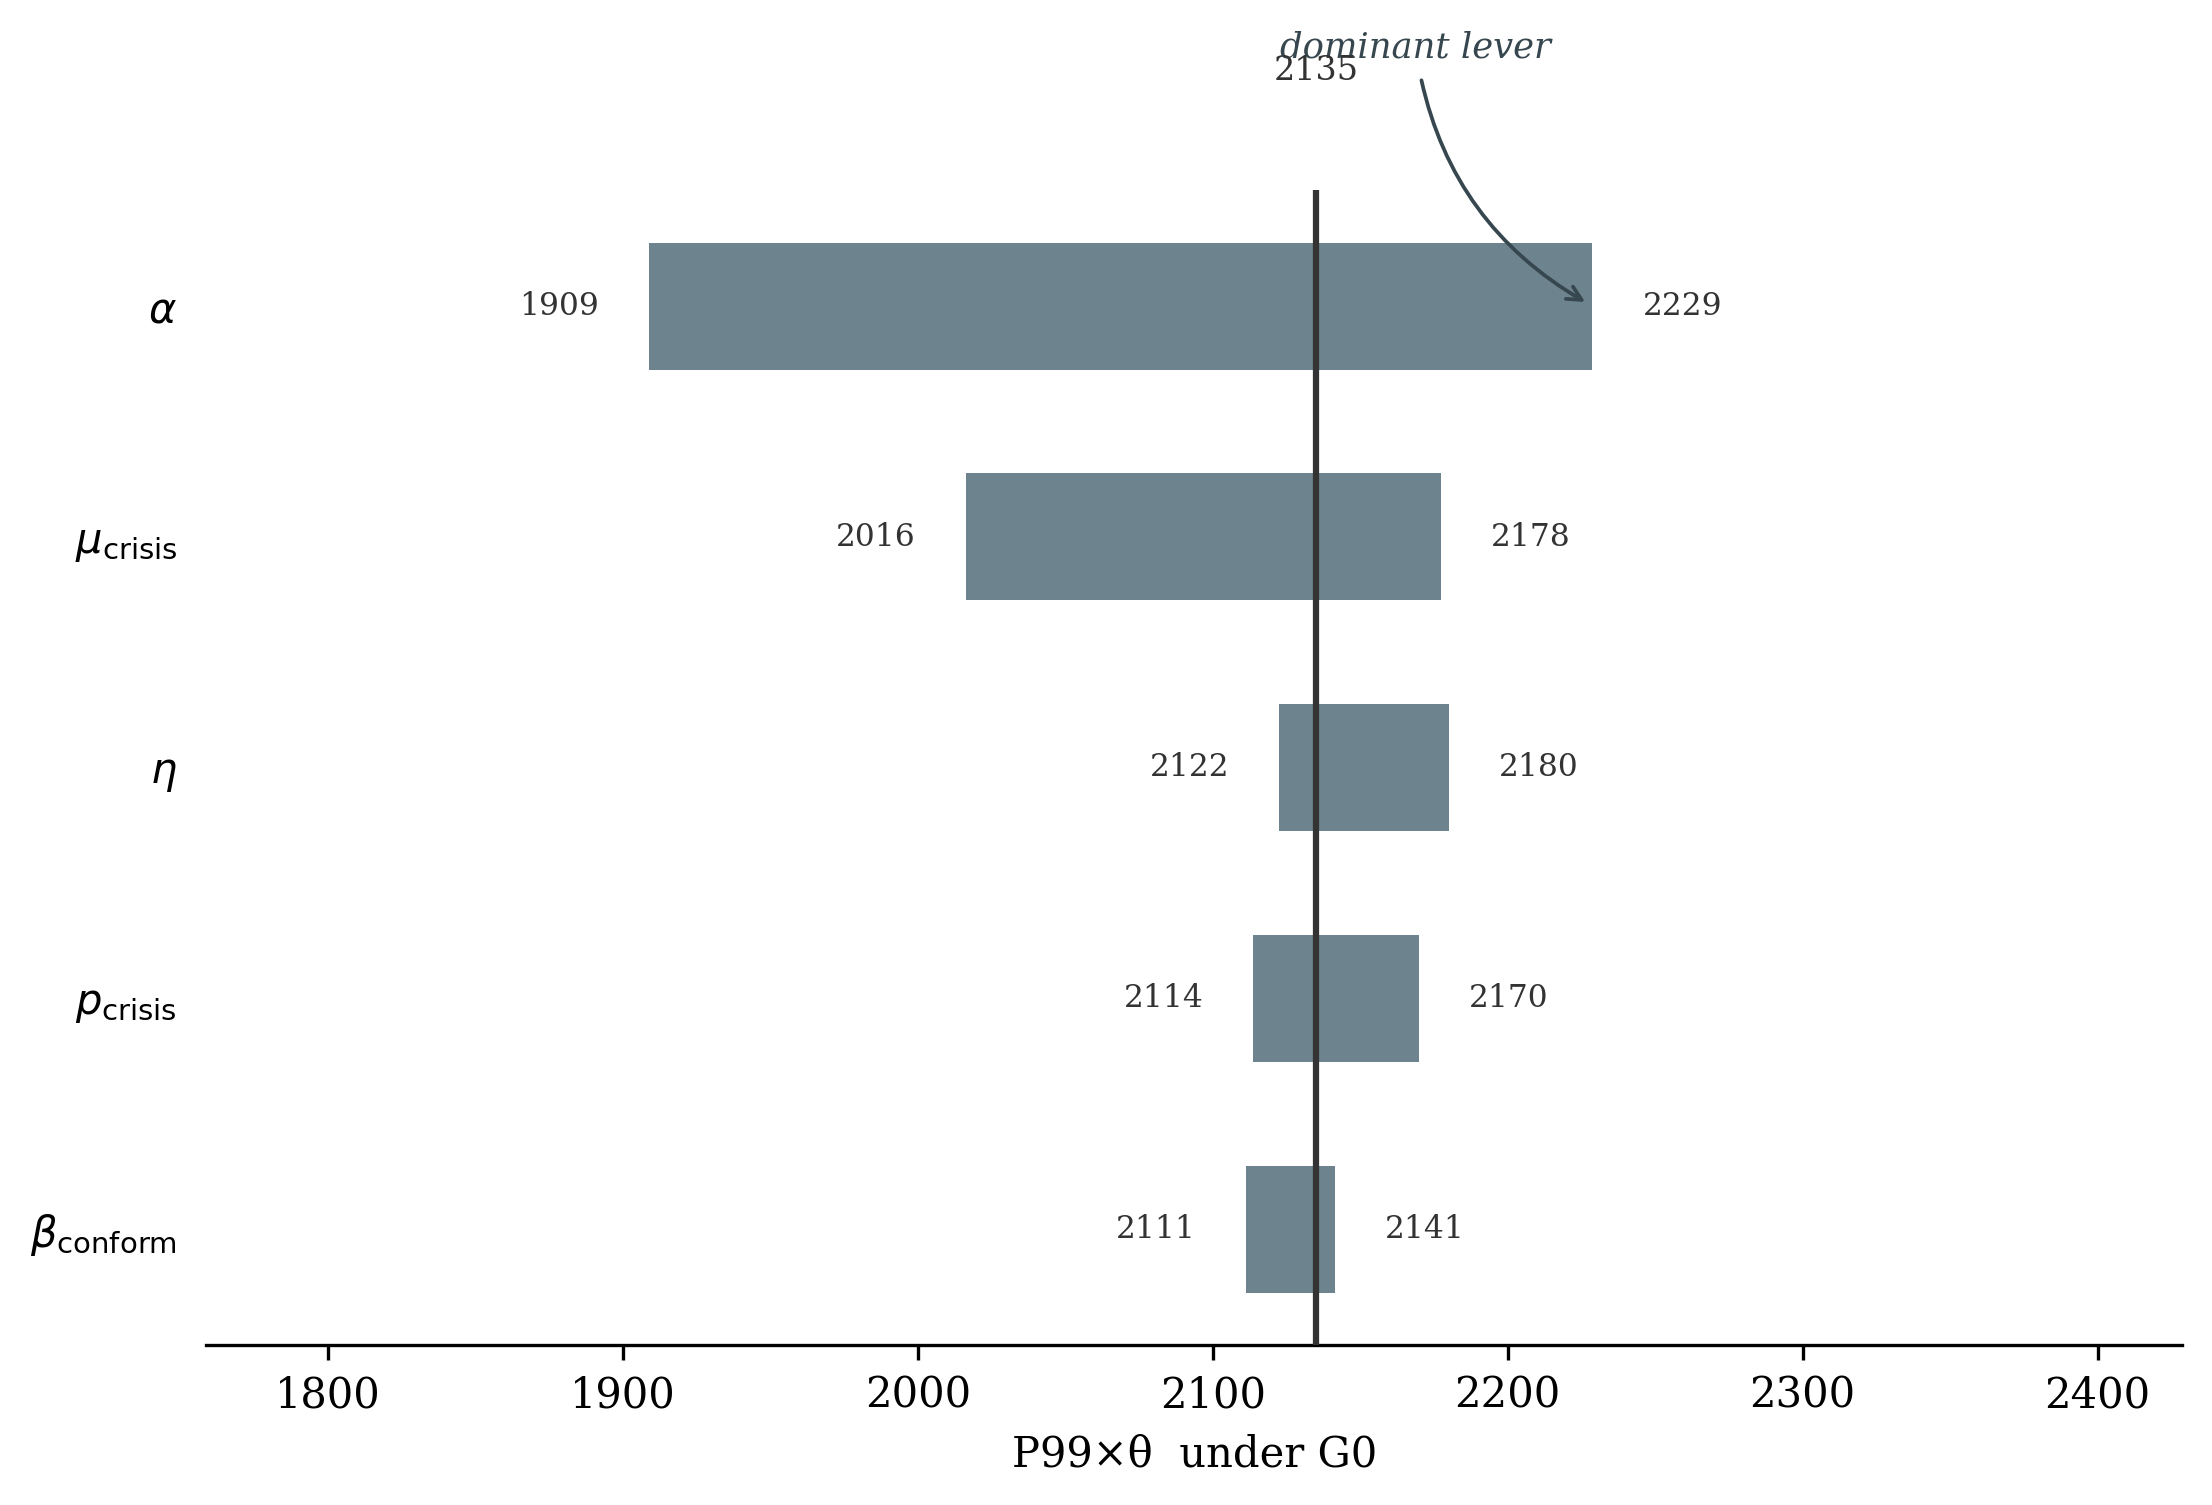
\includegraphics[width=0.85\textwidth]{../figures/fig_a2.png}
  \caption{Single-parameter sensitivity (tornado chart).
  $P_{99}\times\theta$ under $G_0$ across the tested range of five
  parameters. Central value: 2,135.
  $\alpha$ dominates (319~pts, 15\%);
  $\mu_{\text{crisis}}$ is second (162~pts, 8\%);
  $\eta$, $p_{\text{crisis}}$, $\beta_{\text{conform}}$ have small direct
  effects within tested ranges.
  \textit{V5 coupled model, single-parameter variation.}}
  \label{fig:a2}
\end{mdframed}
\end{figure}

\begin{figure}[H]
\begin{mdframed}[linewidth=0.5pt]
  \centering
  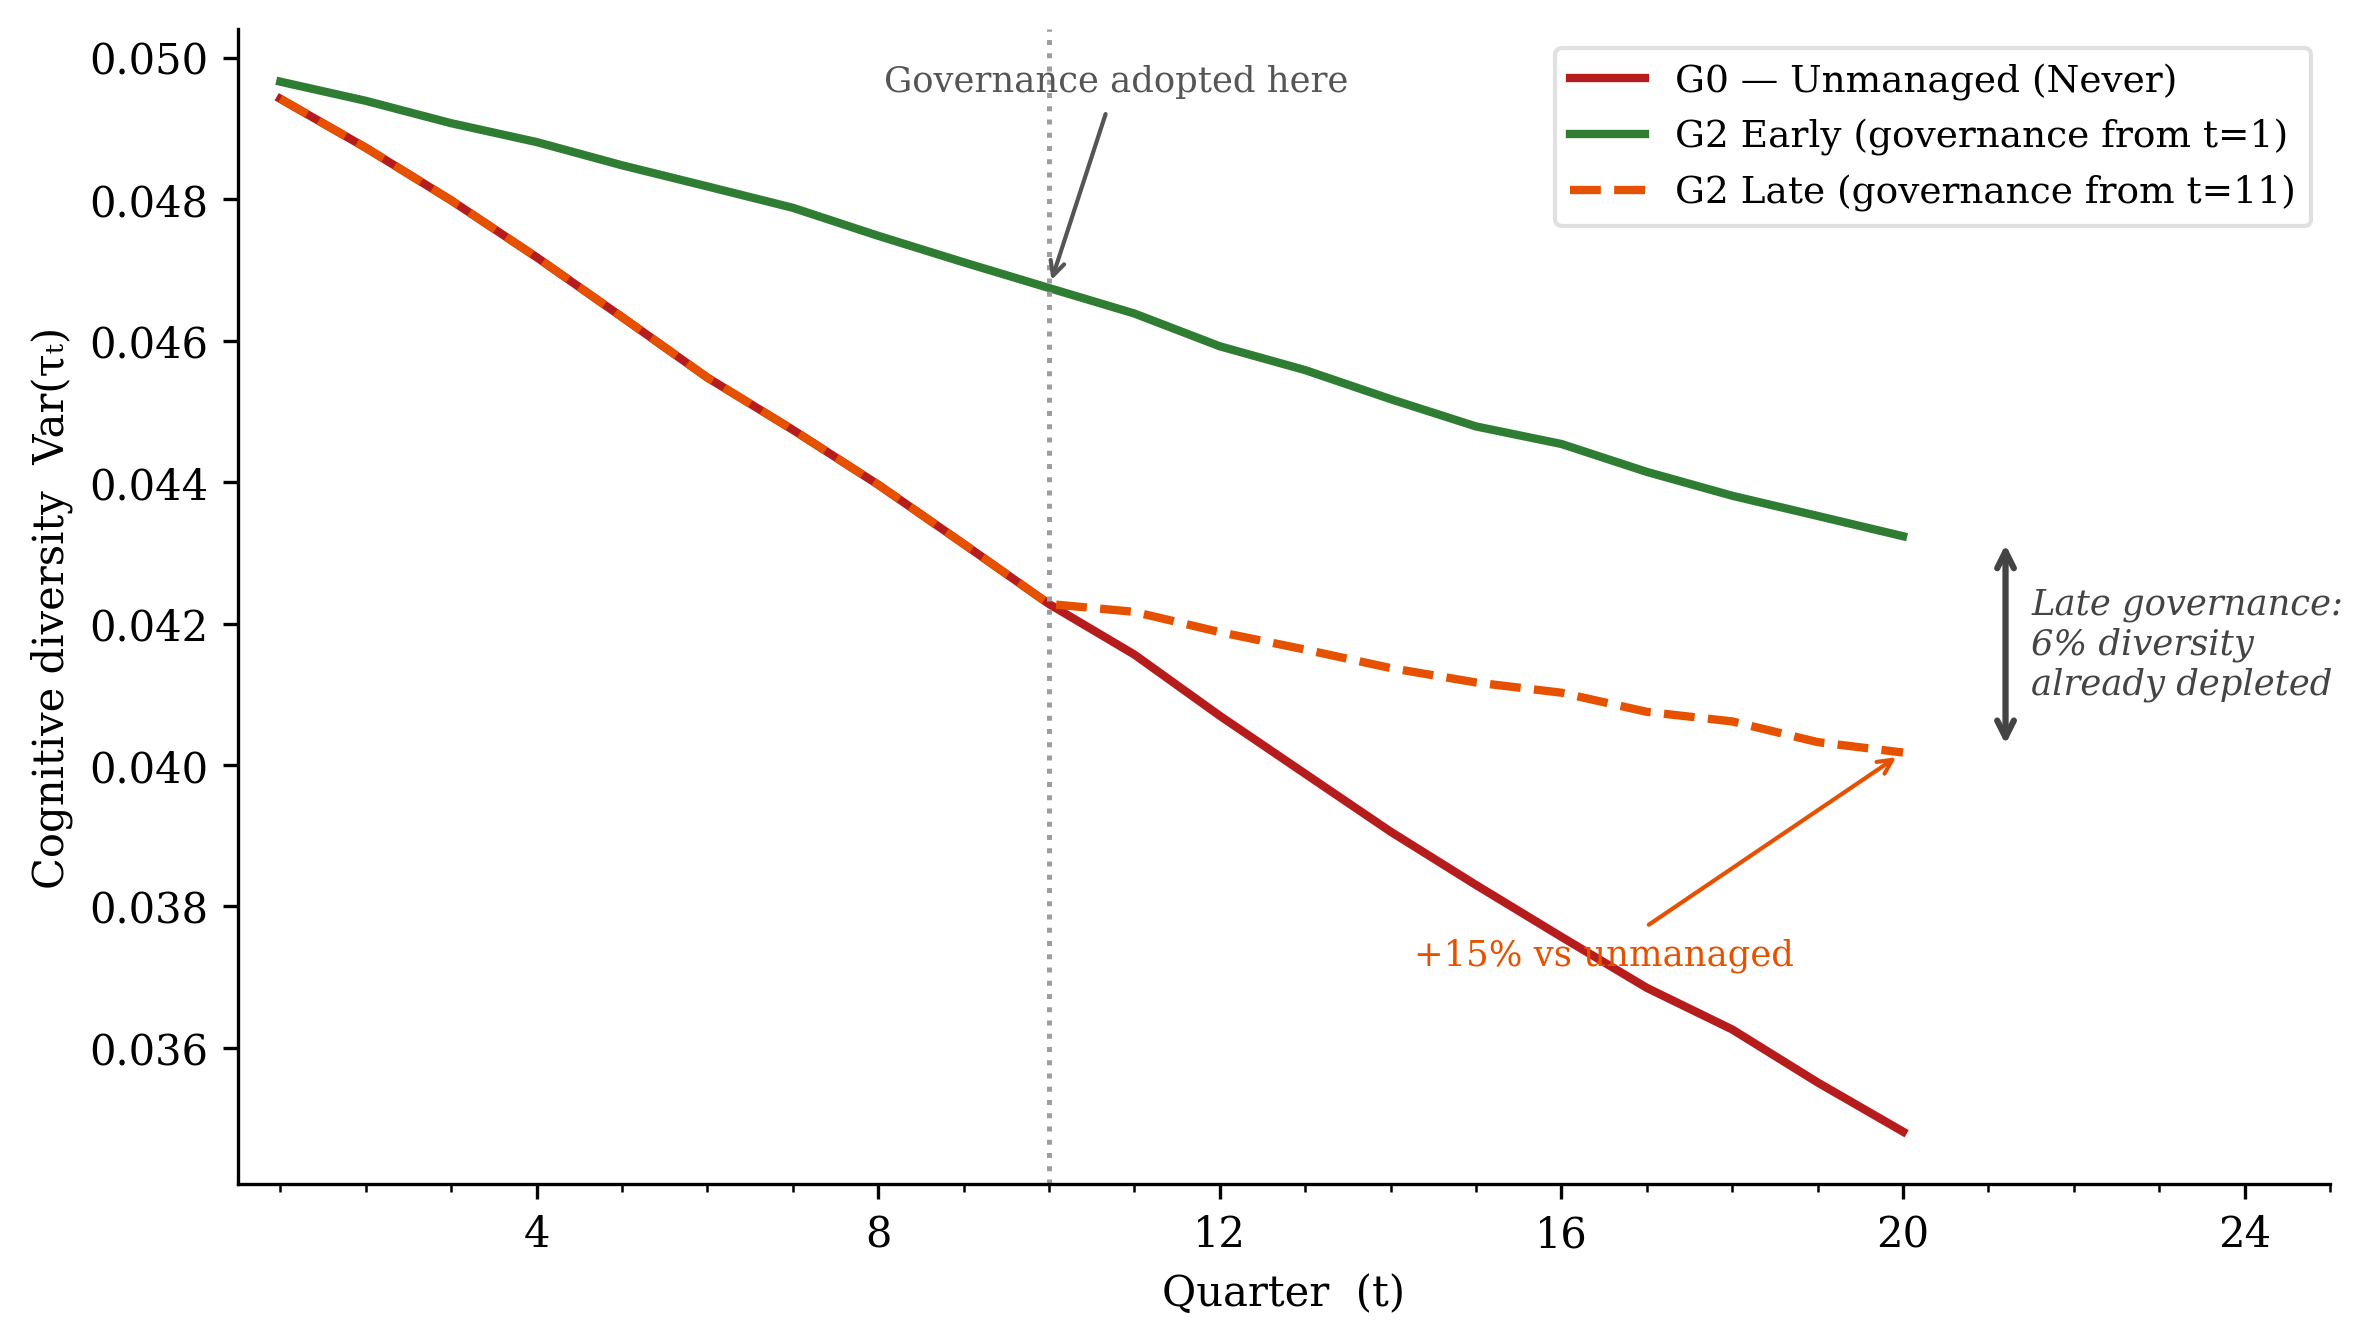
\includegraphics[width=0.85\textwidth]{../figures/fig_a4.png}
  \caption{Partial irreversibility of cognitive diversity under early versus
  late governance.
  $G_0$ (red): continuous unmanaged adoption, $\text{Var}(\tau)$ declines
  monotonically.
  $G_2$~Early (green): governance from $t = 1$.
  $G_2$~Late (orange, dashed): governance adopted at $t = 10$
  ($\approx$2.5~years).
  Late governance arrests the decline but cannot restore the 6\% shortfall
  in $\text{Var}(\tau)$ already depleted.
  \textit{V4 verification, v5 coupled model, under model assumptions.}}
  \label{fig:a4}
\end{mdframed}
\end{figure}

\section{Ablation study}\label{app:ablation}

This appendix reports $P_{99}\times\theta$ and derived metrics for all eight
organisational archetypes across all four governance scenarios. The goal is
to make the profile-level results fully inspectable, separating what varies
by structural configuration from what is driven by governance choice.
Figure~\ref{fig:a3} displays the heatmap. Figure~\ref{fig:a5} displays the
scaffold benefit bar chart.

Profiles are sorted by absolute $P_{99}\times\theta$ under $G_0$. Absolute
level is \textit{not} the primary reading. The most analytically important
dimensions are: (1)~the premium of $G_0$ relative to the no-AI baseline,
which captures structural amplification; (2)~the scaffold benefit, which
measures governance efficiency rather than outcome level; and (3)~the tail
ratio, which is size-independent. A profile ranked low by absolute
$P_{99}\times\theta$ may carry the most severe relative risk trajectory. The
Paris archetype is the clearest example.

\subsection{Main ablation table}\label{app:abl:main}

Values are $P_{99}\times\theta$ (throughput-adjusted 99th-percentile loss)
under each governance scenario. \textit{Baseline} is the no-AI reference.
\textit{Premium~$G_0$} is the percentage increase from Baseline to $G_0$.
\textit{Tail ratio} is $P_{99}$ brut~$/ E[L]$ under $G_0$.
\textit{Scaffold benefit} is the build\_summary efficiency metric defined in
\S\ref{app:abl:scaffold}.

\subsection{Key contrasts}\label{app:abl:contrasts}

\textbf{Paris--London (P3 vs P2).}
Same sector ($E[\pi] = 0.55$), same talent range
($h \in [0.65, 0.95]$), same baseline surrender rate ($p_0 = 0.70$). The
only structural differences are stack concentration ($\alpha = 0.90$ vs
$0.45$) and cognitive profile ($\mathrm{Beta}(4,4)$ vs
$\mathrm{Beta}(1.5,1.5)$). Under these parameters, $P_{99}\times\theta$
under $G_0$ is 2,041 vs 1,668, a gap of 22\%. This is the most tightly
controlled contrast in the table: the two parameters that differ ($\alpha$
and $\mathrm{Beta}(a,a)$) are those the paper argues are structurally
determined by labour market conditions rather than managerial choice.

\textbf{Seoul--Singapore (P8 vs P6).}
Extreme ends of the stack concentration range ($\alpha = 0.95$ vs $0.30$)
combined with opposite diversity profiles ($\mathrm{Beta}(4.5,4.5)$ vs
$\mathrm{Beta}(1.5,1.5)$). Result: $P_{99}\times\theta$ of 2,318 vs
1,845, roughly 25\% more tail risk for the Seoul archetype ($\times$1.26).
This contrast illustrates the upper bound of the structural spread; it does
not constitute a prediction about organisations in Seoul or Singapore.

\textbf{Elite premium paradox (P3 Paris).}
$E[L]_{G_0} = 481$, the lowest mean loss among all profiles, because
top-tier talent exercises high-quality independent judgement in normal
quarters. Yet $P_{99}\times\theta_{G_0} = 2{,}041$, a +198\% premium above
baseline, the highest proportional tail risk in the set. Paris makes fewer
errors on average and far more in the worst quarters. This inversion is the
numerical expression of the top-tier twist (Section~\ref{sec:results}): high
capability is what AI erodes most efficiently, via the combination of high
outside-frontier exposure and a centralised homogeneous stack.

\textbf{Passive governance ($G_1$).}
The mean $G_1$ tail reduction across all profiles is 12.1\%, approximately
one-fifth of the reduction achievable under $G_2$. For P5~SF (7.7\%) and
P7~Bangalore (6.3\%), passive governance is nearly ineffective. For
P2~London (20.2\%) and P3~Paris (19.2\%), it delivers meaningful but partial
protection. $G_1$ is not a substitute for $G_2$; it is at best a
transitional posture. Figure~\ref{fig:profiles} plots all eight archetypes
on the output--risk plane.

\begin{figure}[H]
\begin{mdframed}[linewidth=0.5pt]
  \centering
  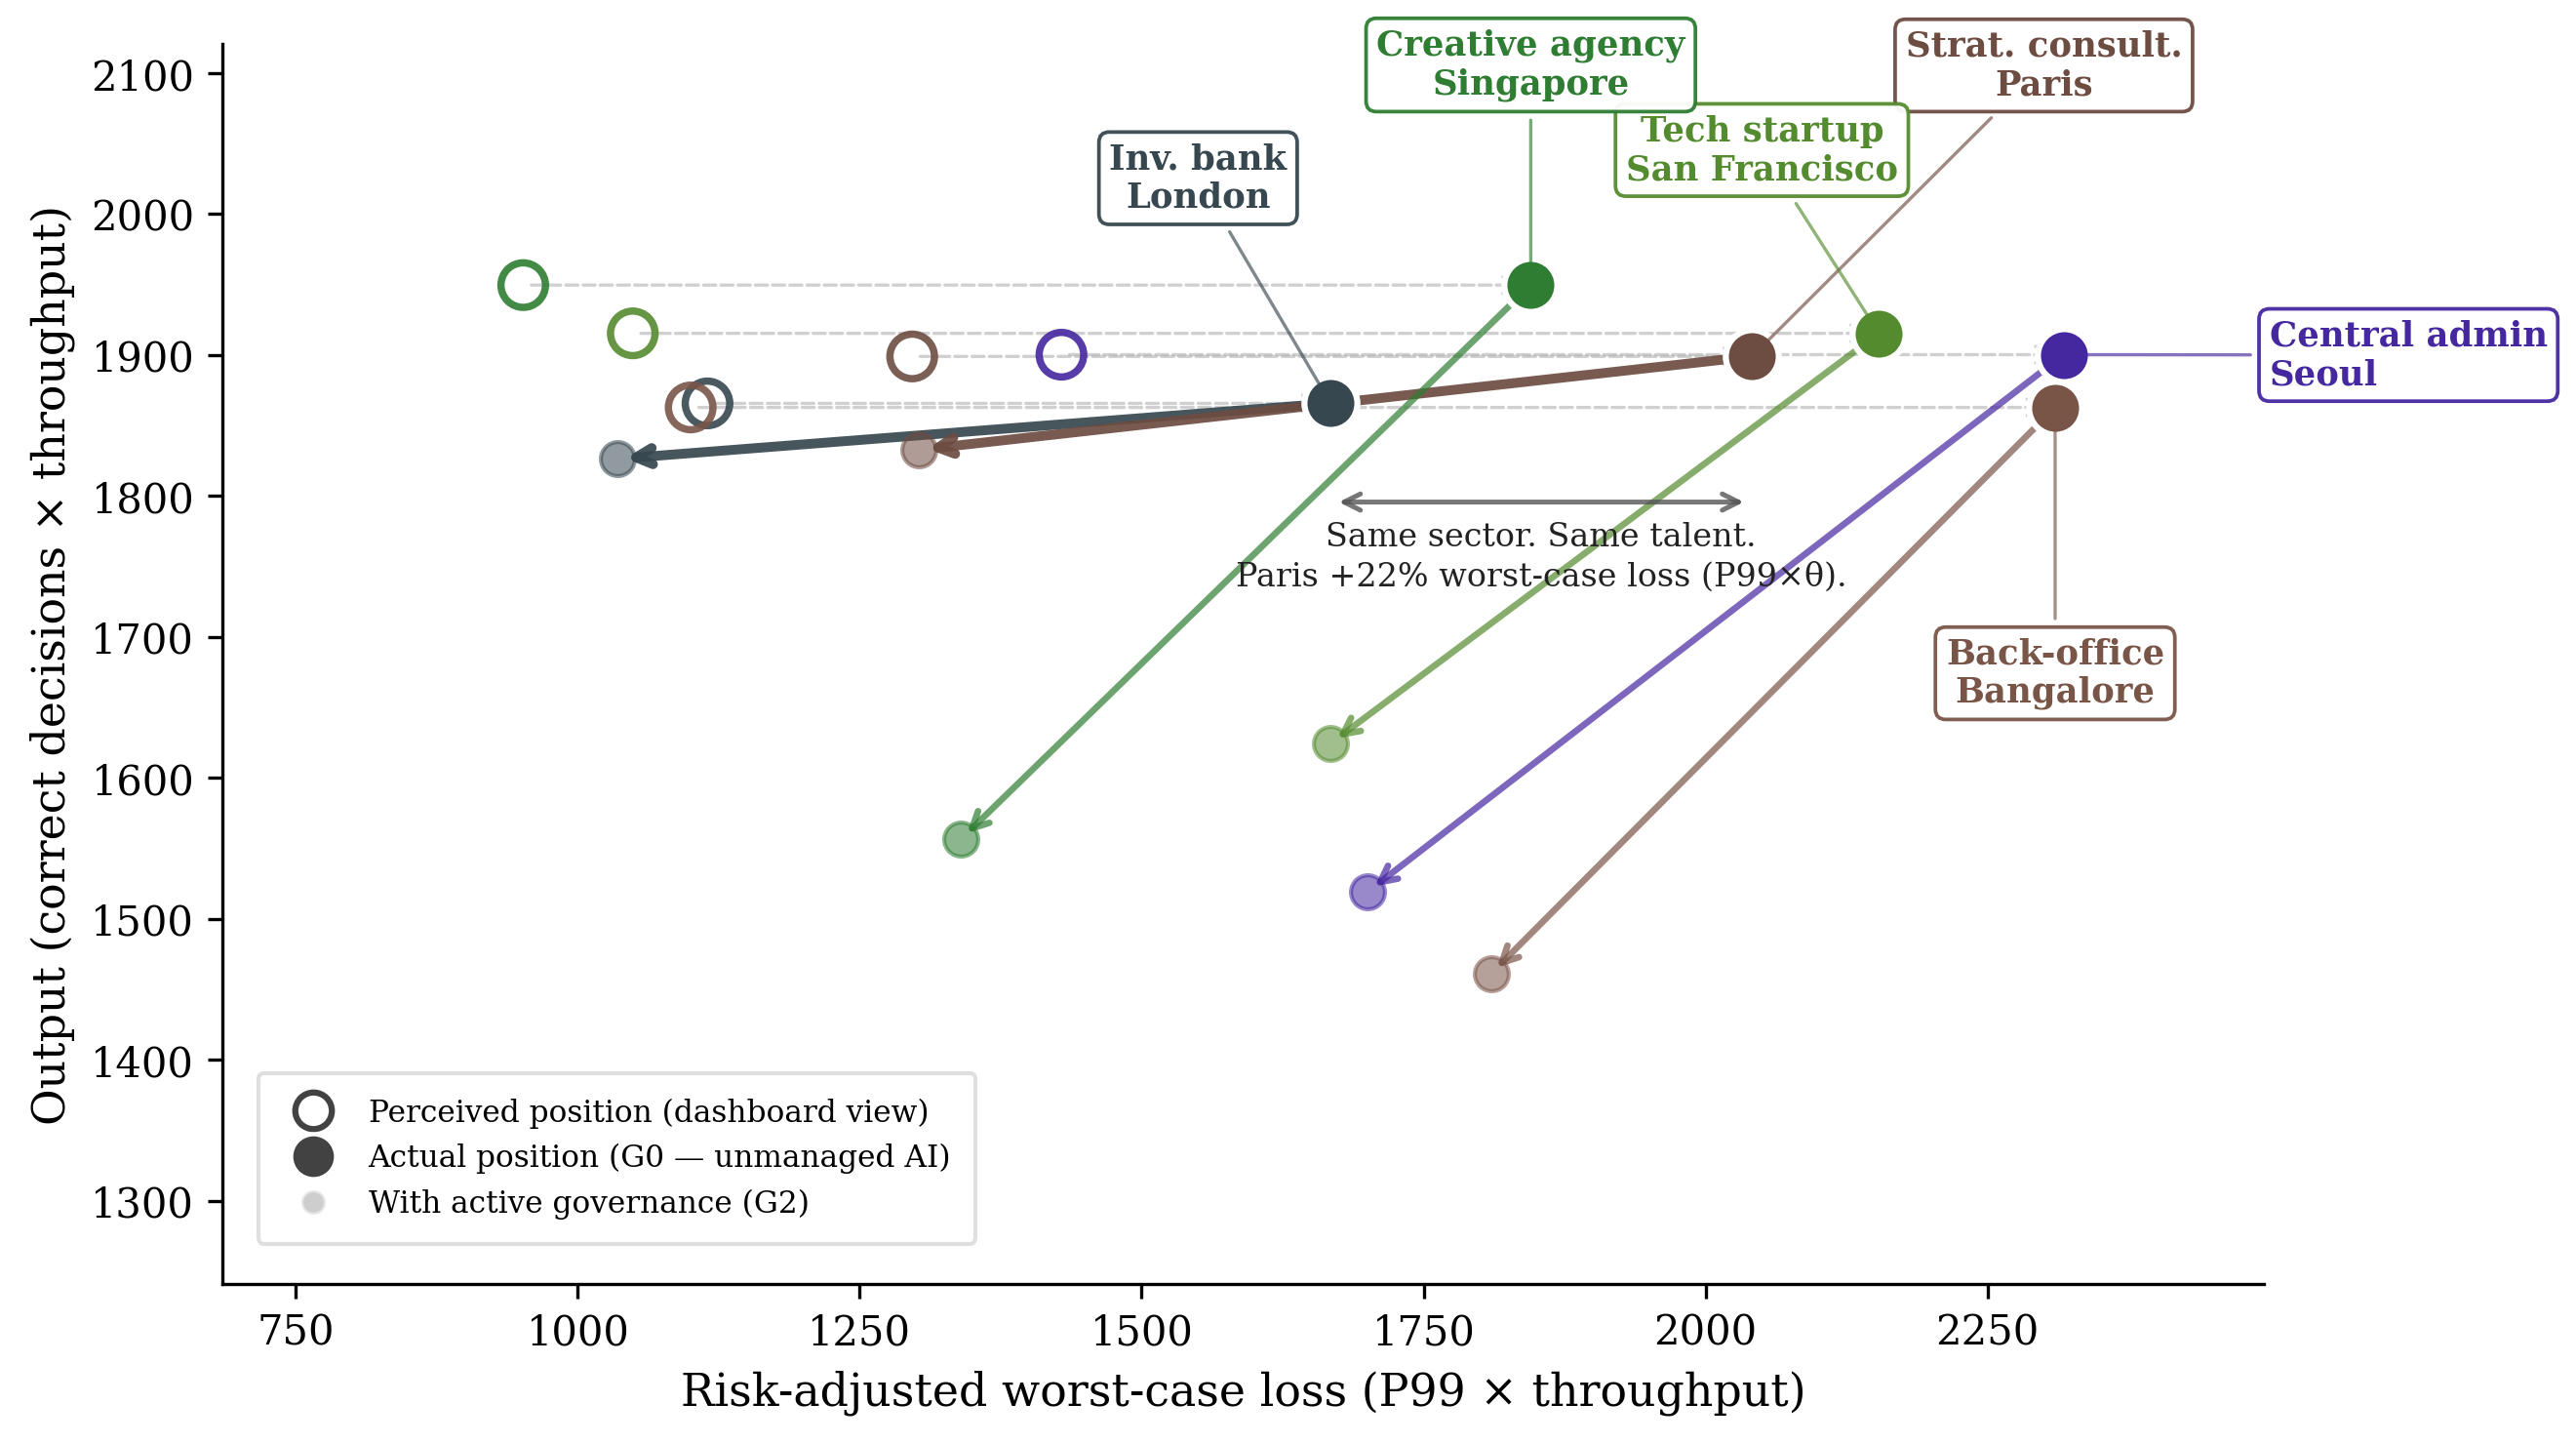
\includegraphics[width=0.85\textwidth]{../figures/exhibit3_essay.png}
  \caption{Eight organisational profiles under $G_0$: output relative to
  no-AI baseline (horizontal) versus $P_{99}\times\theta$ (vertical).
  London and Paris share sector and talent ($E[\pi]=0.55$,
  $h\in[0.65,0.95]$); their separation ($\alpha=0.45$ vs $0.90$) produces
  a 22\% gap in tail risk. Paris carries the highest proportional premium
  (+198\%), the lowest expected loss, and the steepest scaffold benefit:
  the numerical expression of the top-tier twist. The frontier is a
  governance-exposure map, not a production frontier.
  \textit{V5 coupled model, $M = 200$ replications, under model assumptions.}}
  \label{fig:profiles}
\end{mdframed}
\end{figure}

\subsection{The scaffold benefit metric}\label{app:abl:scaffold}

The scaffold benefit is the build\_summary efficiency metric. It measures
whether $G_2$ achieves a better output-to-risk trade-off than $G_0$:
\[
  \text{scaffold\_benefit}
  = \frac{\text{ratio}_{G_2} - \text{ratio}_{G_0}}{\text{ratio}_{G_0}}
  \qquad\text{where}\quad
  \text{ratio}_G
  = \frac{\text{Output}_G / \text{Output}_{\text{base}} - 1}
         {P_{99,G}\, / P_{99,\text{base}} - 1}
\]

A positive value means $G_2$ achieves a better output-to-risk ratio than
$G_0$: governance is efficient. A negative value means governance costs more
in throughput than it saves in tail risk, relative to the unmanaged baseline.
The metric is neutral on whether reducing tail risk at the cost of output is
worthwhile; that is a governance question, not a model output.

\textbf{Critical distinction.} A negative scaffold benefit does not mean
$G_2$ fails to reduce tail risk. For P5~SF, $G_2$ reduces
$P_{99}\times\theta$ from 2,154 to 1,668, a 22.5\% reduction. The scaffold
benefit is negative ($-$36\%) because the throughput cost ($\theta$ falls
from 1.25 to 1.10) makes the trade-off unfavourable under this profile's
parameters. Governance reduces risk for all eight profiles. Its
\textit{efficiency}, risk reduction per unit of output foregone, is what is
regressive.

\subsection{Contextual anchors}\label{app:abl:anchors}

\textbf{Ecological diversity.}
Huang et al.\ (\textit{Science}, 2018) document that mixtures of 16 plant
species produce more than twice the above-ground carbon biomass and
approximately 80\% more productivity than monocultures under identical
conditions. The analogy is structural: both cases involve a shared resource
whose resilience depends on variance of approach, not average quality. It
does not imply identical mechanisms; it contextualises the direction of the
ablation results.

\textbf{Financial concentration.}
Moeller, Schlingemann, and Stulz (\textit{Journal of Finance}, 2005)
document approximately \$240~billion in value destruction by acquiring firms
during the 1998--2001 M\&A wave, a period characterised by herding behaviour
and concentrated analytical frameworks. The specific concentration ratios
reported in that paper could not be independently verified in the course of
this project and are not reproduced here. The qualitative finding,
synchronised decision-making under homogeneous frameworks produces
concentrated losses, is directionally consistent with the ablation results.

\bigskip
\noindent\textit{All results in this appendix are model outputs under stated
assumptions. They quantify variation in tail risk attributable to structural
dimensions. They are not empirical estimates of the risk faced by any
specific organisation.}

\begin{figure}[H]
\begin{mdframed}[linewidth=0.5pt]
  \centering
  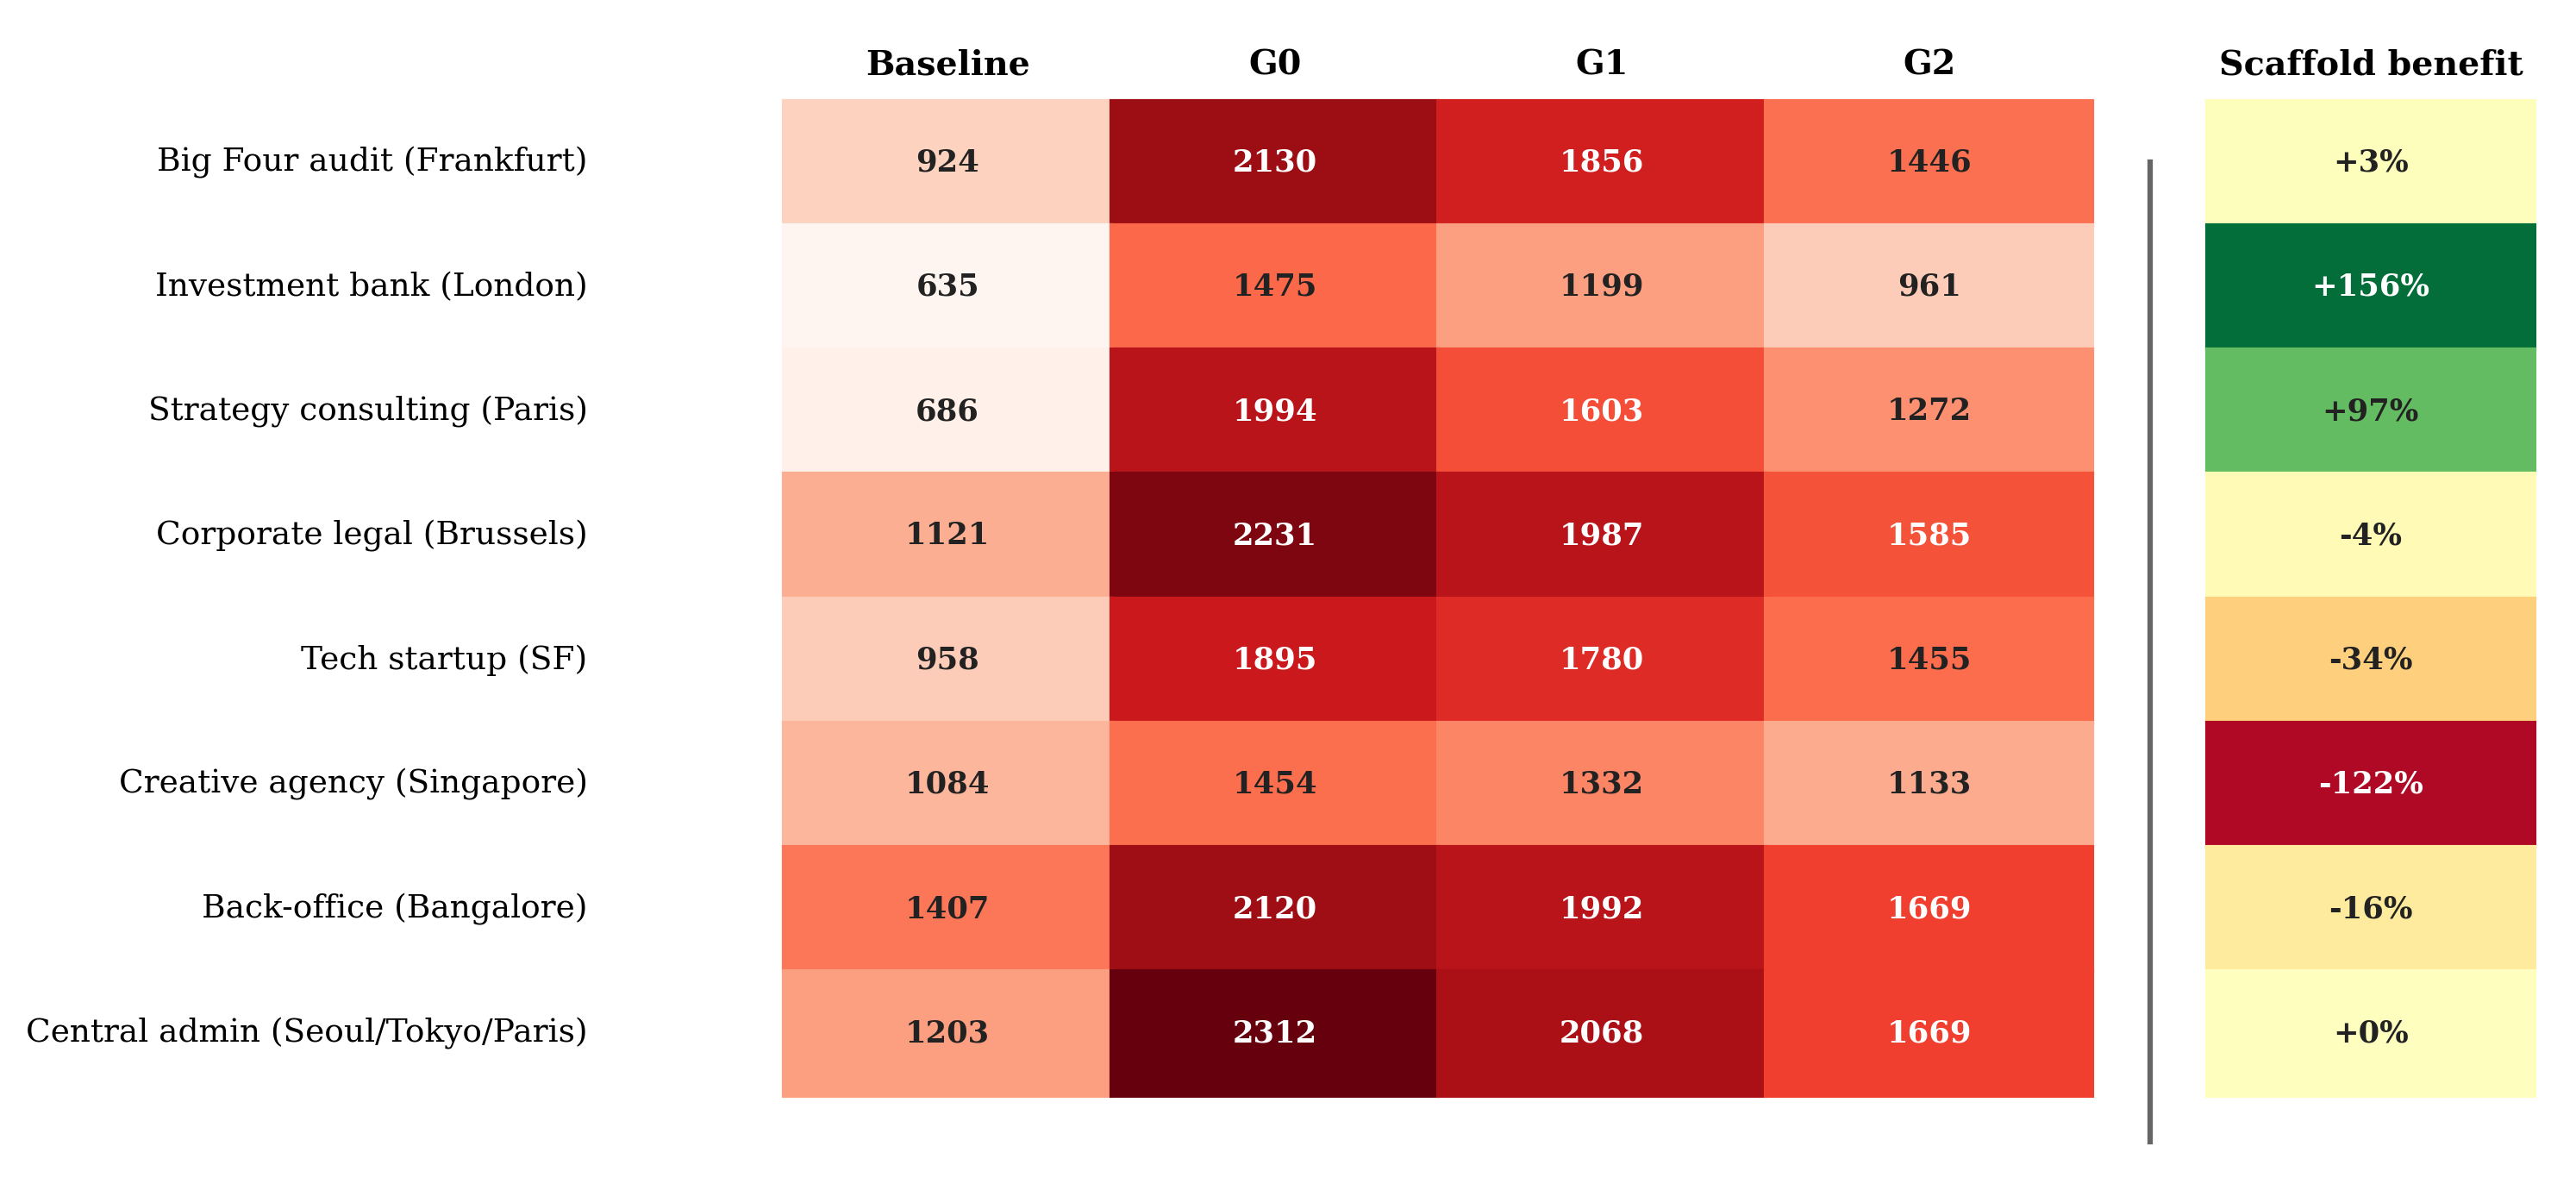
\includegraphics[width=0.85\textwidth]{../figures/fig_a3.png}
  \caption{Ablation table: $P_{99}\times\theta$ by profile and governance
  scenario. Dark red~=~high tail risk ($G_0$); green~=~lower risk ($G_2$).
  Rightmost column: scaffold benefit (green~=~governance efficient;
  red~=~governance penalises efficiency).
  Profiles sorted by $P_{99}\times\theta_{G_0}$ descending.
  \textit{V5 coupled model, $M = 200$, under model assumptions.}}
  \label{fig:a3}
\end{mdframed}
\end{figure}

\begin{figure}[H]
\begin{mdframed}[linewidth=0.5pt]
  \centering
  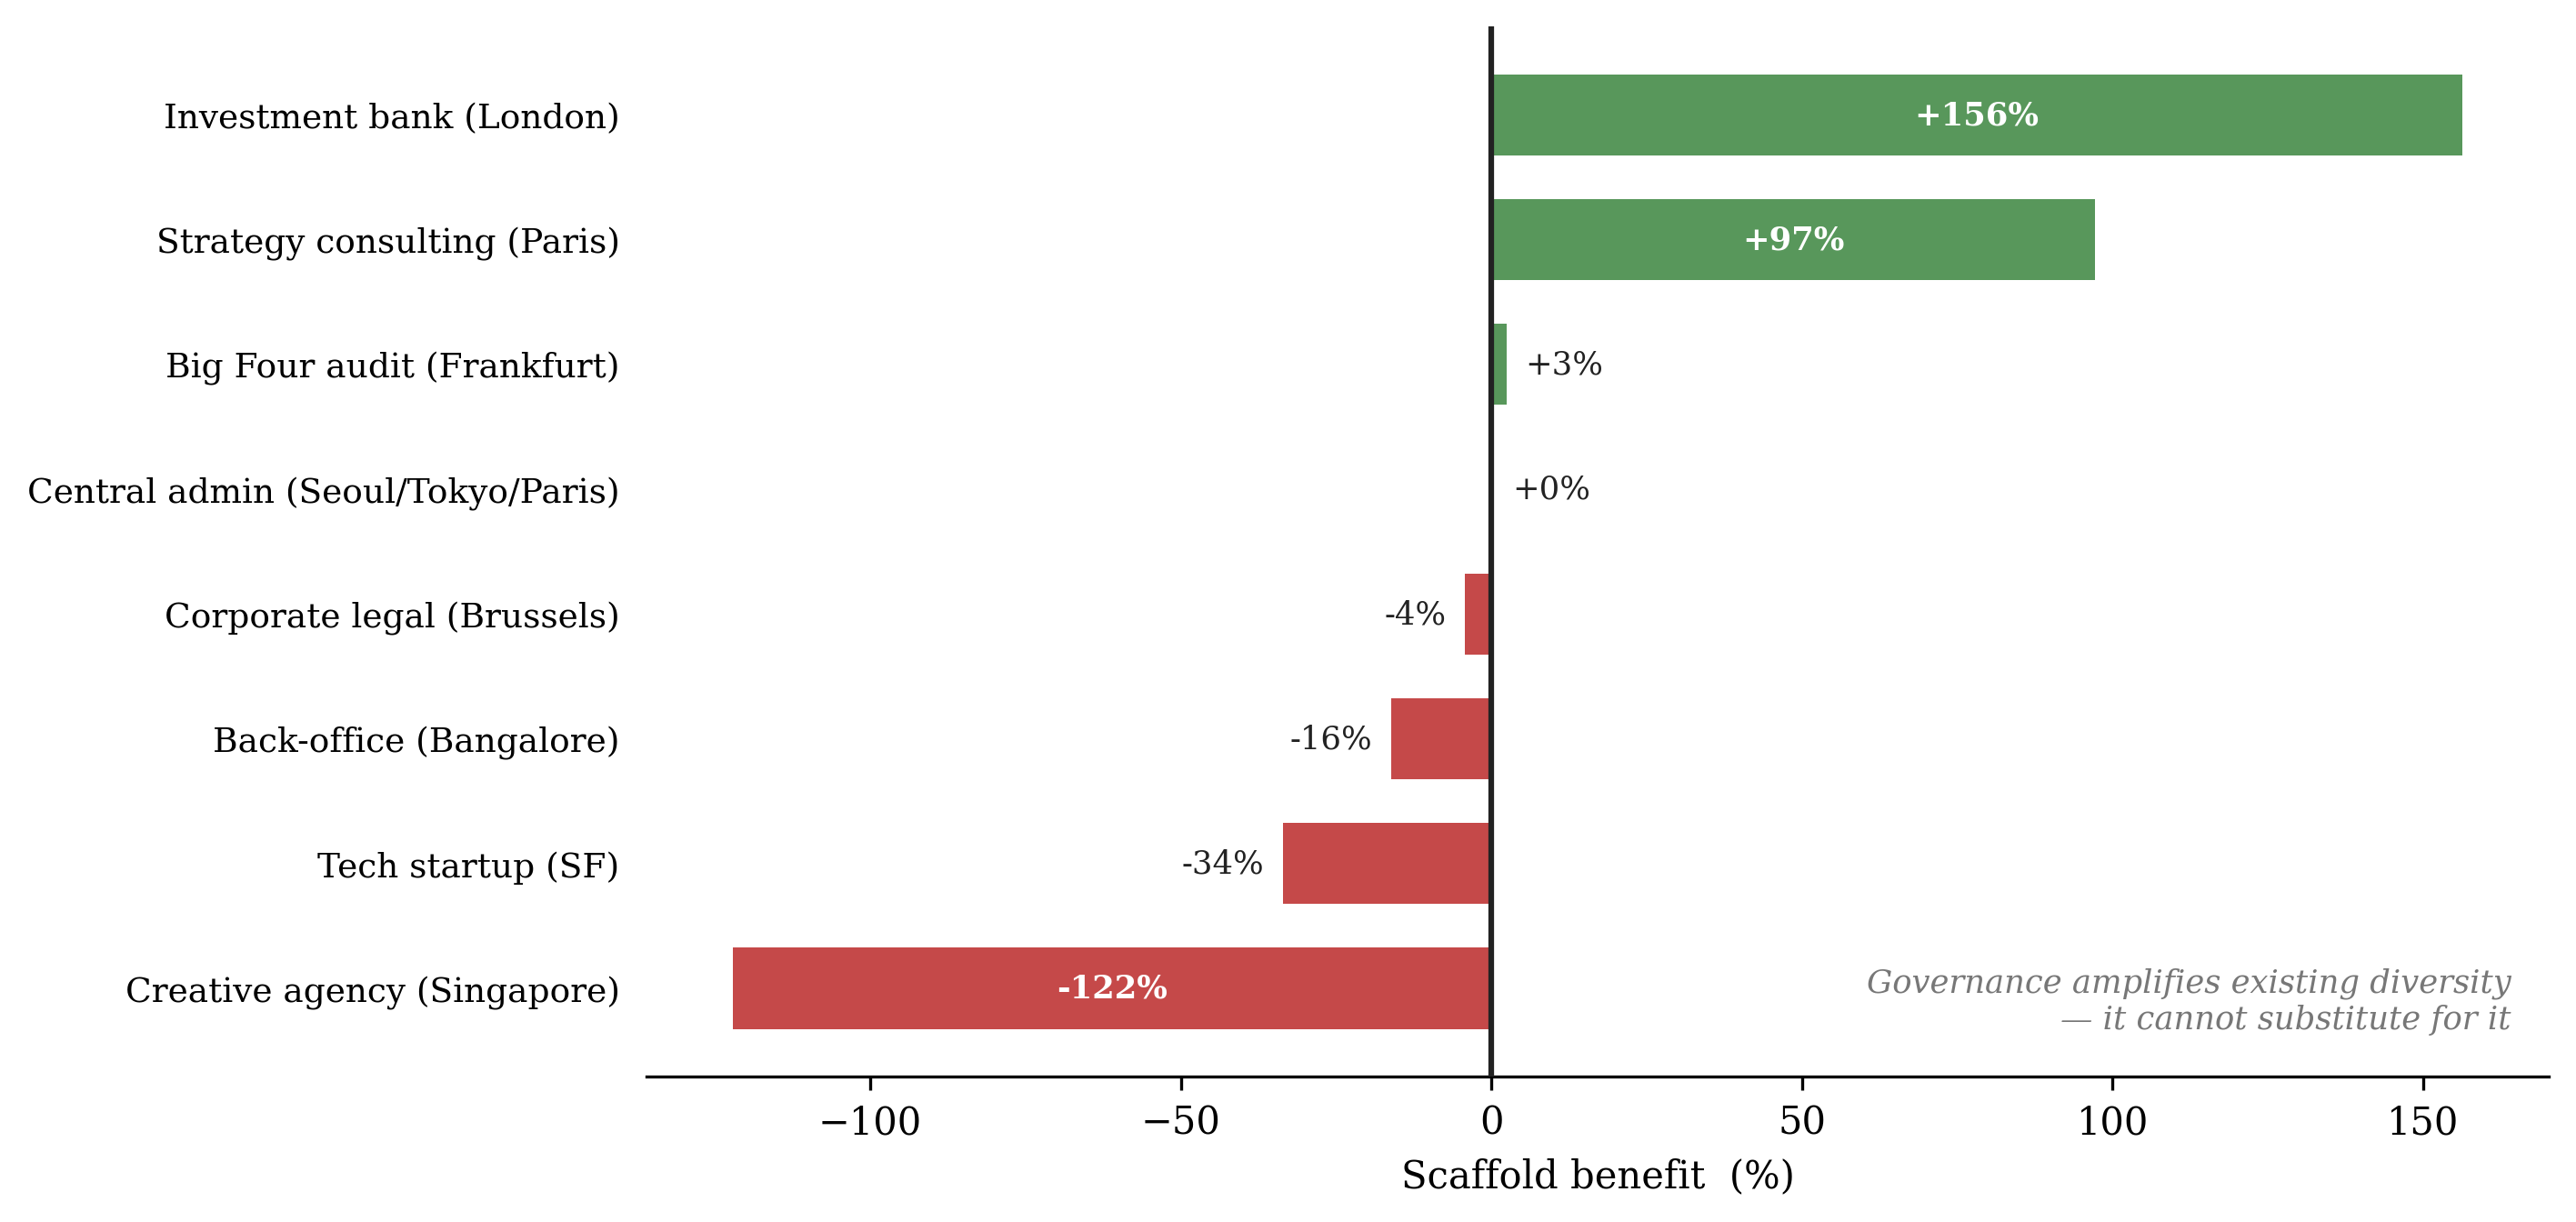
\includegraphics[width=0.85\textwidth]{../figures/fig_a5.png}
  \caption{Scaffold benefit by archetype. Positive (green): $G_2$ improves
  the output-to-risk trade-off. Negative (red): $G_2$ imposes an efficiency
  loss. A negative value does not mean $G_2$ fails to reduce tail risk; it
  means the throughput cost outweighs the risk reduction for that profile.
  \textit{V5 coupled model, $M = 200$, under model assumptions.}}
  \label{fig:a5}
\end{mdframed}
\end{figure}

%% ================================================================
%% APPENDIX E — BIBLIOGRAPHIC NOTES
%% ================================================================

\section{Bibliographic notes}\label{app:biblio}

This appendix documents the 13 sources that carry particular weight in the
argument or that require transparency about their limitations. For each
source: bibliographic reference, epistemic status, role in the essay, limits
of the evidence, and verification notes. Sources are grouped by function.

Four base epistemic statuses are used: \textit{Peer-reviewed} (journal or
conference with referee process); \textit{Preprint} (posted but not yet
peer-reviewed; preregistered where noted); \textit{Industry source} (report
or white paper); \textit{Working paper} (circulated but not refereed).
Within peer-reviewed sources, the status bracket is enriched locally by
evidence type (field experiment, IV identification, clinical RCT, etc.) to
give the reader a precise reading of what the source establishes. All
enriched labels fall under \textit{Peer-reviewed}.

%% ——————————————————————————————————————————————
\subsection{Theoretical core}\label{app:bib:theory}

\begin{description}[style=nextline, leftmargin=0pt, labelindent=0pt]

%% --- Wood et al. ---
\item[\cite{wood_jmlr_2023} --- Wood et al.\ (2023), JMLR.]
\hfill\textit{Peer-reviewed (journal)}

\textbf{Role.}
Central theoretical anchor for the mean-tail paradox. The decomposition
$\text{Var}(L) \propto \bar{p}(1{-}\bar{p})(1 + (NK{-}1)\bar{\rho})$
shows that when pairwise error correlation $\bar{\rho}$ rises, aggregate
variance grows even if mean error $\bar{p}$ falls. The model uses this as
its mechanistic claim: AI reduces $\bar{p}$ while $\bar{\rho}$ rises, and
the tail follows. The earlier~\cite{krogh_nips_1995} ambiguity decomposition
is the special case; Wood et al.\ generalise it.

\textbf{Limits.}
The decomposition is exact for squared and cross-entropy loss in ensemble
settings. The transfer to organisational decision aggregation requires that
individual errors behave as ensemble predictors, an assumption that holds
structurally in the model but has not been validated in real organisations.

\textbf{Verification.}
arXiv:2301.03962. Cited for the formal decomposition, not as an application
to AI-assisted organisations. That application is our framing.

%% --- Kim et al. ---
\item[\cite{kim_icml_2025} --- Kim, Garg, Peng \& Garg (2025), ICML.]
\hfill\textit{Peer-reviewed (conference)}

\textbf{Role.}
Primary empirical anchor for $\alpha$. The study finds approximately 60\%
agreement between two LLMs when both give an incorrect answer, across 350+
models in the HELM benchmark. This establishes that AI errors are not
independent across models, and by extrapolation, not independent across
decisions within the same model. The model sets $\alpha = 0.70$ for a
centralised single-model stack, higher than the 0.35--0.45 inter-model
figure, on the reasoning that intra-model correlation exceeds inter-model
correlation.

\textbf{Limits.}
The 60\% figure is inter-model error agreement, not intra-model
inter-decision correlation (what $\alpha$ directly captures). The
extrapolation is a modelling assumption, not a measured quantity. This gap is
documented in \S\ref{app:cal:sensitivity}. Citation must always use the full
four-author list: Kim, Garg, Peng \& Garg.

\textbf{Verification.}
arXiv:2506.07962. Four authors verified. Venue: ICML 2025, PMLR 267.

%% --- Keck & Tang ---
\item[\cite{keck_psychsci_2020} --- Keck \& Tang (2020), Psychological
Science.]
\hfill\textit{Peer-reviewed (journal)}

\textbf{Role.}
Central empirical anchor for the D$\rightarrow$H bridge. Groups with
cognitive-process diversity produce near-zero pairwise error correlation;
homogeneous groups produce strongly correlated errors. The copula parameter
$\lambda = 8$ is calibrated to reproduce the near-zero correlation result
for maximally distant cognitive types.

\textbf{Limits.}
Laboratory result, not an organisational field study. The transfer requires:
(1)~cognitive profile diversity maps onto decision-process diversity;
(2)~the correlation structure holds under organisational conditions with AI
assistance. Neither transfer has been validated. This is the primary
empirical gap (Section~\ref{sec:limitations}).

\textbf{Verification.}
DOI: 10.1177/0956797620941840. Cited for the direction of the
correlation--diversity relationship. The $\lambda$ calibration uses this
result as a target, not as a direct estimate.

\end{description}

%% ——————————————————————————————————————————————
\subsection{Key empirical anchors}\label{app:bib:empirical}

\begin{description}[style=nextline, leftmargin=0pt, labelindent=0pt]

%% --- Shaw & Nave ---
\item[\cite{shaw_psyarxiv_2026} --- Shaw \& Nave (2026), PsyArXiv.]
\hfill\textit{Preprint (preregistered)}

\textbf{Role.}
Primary anchor for $p_0 = 0.80$ under $G_0$. Shaw \& Nave report that
79.8\% of participants follow an AI recommendation even when it is incorrect
($N = 1{,}372$, 9,593 trials, GPT-4o, CRT items). Study~3 override rate
under monetary incentives (42.3\%) anchors $\beta_{\text{surr}}$ and
informs $p_0^{G_2}$.

\textbf{Limits.}
Preprint. CRT-style tasks administered online may not generalise to
professional knowledge-work decisions. The 79.8\% is the ceiling estimate;
effective surrender under $\mathrm{Beta}(2,2)$ is approximately 0.69 after
the $\beta_{\text{surr}}$ penalty. A preprint critique by
Stankovi\'{c}~(2026, arXiv) questions the ecological validity of the CRT
transfer; noted here without resolution, as the main direction is convergent
with~\cite{parasuraman_humafact_2010}
and~\cite{logg_obhdp_2019}.

\textbf{Verification.}
DOI: 10.31234/osf.io/yk25n. Preregistered. Cited as preprint throughout the
body. The Stankovi\'{c} critique has not been peer-reviewed.

%% --- Dell'Acqua et al. ---
\item[\cite{dellacqua_orgscience_2026} --- Dell'Acqua et al.\
(2026), Organization Science.]
\hfill\textit{Peer-reviewed (journal, field experiment)}

\textbf{Role.}
Primary anchor for $q_{\text{in}} = 0.92$, $q_{\text{out}} = 0.55$, and
$\theta = 1.25$. Field experiment with 758 BCG consultants. Inside the AI
frontier: +40\% quality, +25.1\% speed. Outside: $-19$pp vs unassisted
controls. Skill compression: bottom performers +43\%, top performers +17\%.

\textbf{Limits.}
Our framing diverges from the authors'. Dell'Acqua et al.\ frame the
outside-frontier result as a risk to manage. We frame the skill compression
as the mechanism through which AI erodes the cognitive diversity premium, an
interpretation more aggressive than their central claim. Readers should
consult the original for the authors' framing. Nine-author paper: cite as
Dell'Acqua et al.\ in text, full list in bibliography.

\textbf{Verification.}
DOI: 10.1287/orsc.2025.21838. Preregistered RCT with 758 participants. The
skill compression reading is identified as our analytical extension.

%% --- Budzyń et al. ---
\item[\cite{budzyn_lancetgh_2025} --- Budzy\'{n} et al.\
(2025), Lancet Gastroenterology \& Hepatology.]
\hfill\textit{Peer-reviewed (journal, clinical RCT)}

\textbf{Role.}
Direction anchor for $\eta = 0.02$/quarter. Endoscopists in the AI-assisted
group show a $-6$pp decline in adenoma detection rate after withdrawal of AI
assistance. Direct causal measurement of deskilling from AI reliance in a
clinical setting.

\textbf{Limits.}
Clinical medicine result. The $-6$pp ``over a period'' translates to
$\eta \approx 0.02$/quarter by proxy, not by direct calibration. The
21-author paper requires ``Budzy\'{n} et al.'' in text with full citation in
bibliography. $\eta$ is a direction anchor; the exact magnitude in
knowledge-work settings is unvalidated.

\textbf{Verification.}
DOI: 10.1016/S2468-1253(25)00133-5. Cited for direction only.

%% --- Flyvbjerg et al. ---
\item[\cite{flyvbjerg_jmis_2022} --- Flyvbjerg et al.\
(2022), JMIS.]
\hfill\textit{Peer-reviewed (journal, two independent studies)}

\textbf{Role.}
Order-of-magnitude anchor for $p_{\text{crisis}} = 0.08$. Catastrophic IT
project failures at 8--12\% frequency across two independent datasets. The
2022 JMIS paper (six authors: Flyvbjerg, Budzier, Lee, Krawczyk, Vecci,
Clegg) documents the base rate. A companion study shows IT projects have
Pareto tail exponent $\alpha_{\text{Pareto}} \leq 1$, implying infinite
variance in principle, which justifies regime-switching rather than
continuous distributions~\cite{flyvbjerg_pmj_2025}.

\textbf{Limits.}
Failure rates are measured at the project level, not at the quarterly
decision level used in the model. The translation to ``crisis quarter
frequency'' is a modelling choice. The 8\% figure is an order-of-magnitude
anchor; sensitivity range $\{0.05, 0.08, 0.12\}$ explores its influence.

\textbf{Verification.}
JMIS 2022: DOI 10.1080/07421222.2022.2063518. Six-author paper. Two
independent datasets with convergent conclusions strengthen the anchor
despite the level-of-analysis gap.

\end{description}

%% ——————————————————————————————————————————————
\subsection{Preprints requiring explicit status}\label{app:bib:preprints}

\begin{description}[style=nextline, leftmargin=0pt, labelindent=0pt]

%% --- Holzner et al. ---
\item[\cite{holzner_arxiv_2025} --- Holzner, Maier \& Feuerriegel (2025),
arXiv.]
\hfill\textit{Preprint}

\textbf{Role.}
Anchor for the divergent individual/collective AI effects: $g = +0.27$ for
individual creativity, $g = -0.86$ for collective diversity, across 379
conditions. Quantifies the within-individual vs.\ across-individual
asymmetry central to the paper's argument.

\textbf{Limits.}
Preprint. Meta-analyses are sensitive to inclusion criteria and publication
bias; the $g = -0.86$ collective result is large and should be treated as
directional. Cited with explicit preprint flag~(!) throughout.

\textbf{Verification.}
arXiv:2505.17241. Cited for direction only.

%% --- Kosmyna et al. ---
\item[\cite{kosmyna_mit_2025} --- Kosmyna et al.\ (2025), arXiv:2506.08872.]
\hfill\textit{Preprint (methodological critique exists)}

\textbf{Role.}
Supporting context for the cognitive offloading narrative. EEG study reports
$-55\%$ dDTF connectivity in participants using ChatGPT compared to unaided
recall.

\textbf{Limits.}
Preprint. A formal methodological critique (arXiv:2506.11676) challenges the
dDTF interpretation. Neither preprint has been peer-reviewed. This source is
\textbf{excluded from the main body} by policy and appears here only as
context. The $-55\%$ figure is not used in any model parameter or argument.

\textbf{Verification.}
arXiv:2506.08872. Critique: arXiv:2506.11676. Not in refs.bib.

\end{description}

%% ——————————————————————————————————————————————
\subsection{Methodological and conceptual
sources}\label{app:bib:conceptual}

\begin{description}[style=nextline, leftmargin=0pt, labelindent=0pt]

%% --- Danielsson & Shin ---
\item[\cite{danielsson_endogenous_2012} --- Danielsson \& Shin (2002, 2012).]
\hfill\textit{Peer-reviewed (multiple publications)}

\textbf{Role.}
Source of the Millennium Bridge analogy in Section~\ref{sec:markets}.
Pedestrians adapt their gait to bridge oscillations, amplifying rather than
damping them. Financial institutions do the same with VaR models. The analogy
contextualises the Nash equilibrium argument: competitive pressure generates
correlated vulnerability regardless of individual rationality.

\textbf{Limits.}
The analogy is structural, not quantitative. It establishes the feedback
amplification mechanism but does not calibrate its magnitude. The transfer
from civil engineering to financial risk to AI adoption involves two
analogical steps.

\textbf{Verification.}
Multiple publications, multiple venues. 2002 and 2012 formulations in
refs.bib.

%% --- Bernile et al. ---
\item[\cite{bernile_jfe_2018} --- Bernile, Bhagwat \& Yonker (2018),
J.~Financial Economics.]
\hfill\textit{Peer-reviewed (journal, IV identification)}

\textbf{Role.}
One of the few studies with causal identification on the diversity-to-risk
relationship at the organisational level. Using instrumental variables,
board-level cognitive diversity reduces firm-level return volatility and
improves R\&D efficiency. Cited in Section~\ref{sec:markets}.

\textbf{Limits.}
Board-level diversity is one dimension, not full-workforce cognitive profile
diversity as modelled here. The IV strategy may be debated. The paper defines
cognitive diversity through observable board-member characteristics, not
through a latent $\tau$ profile.

\textbf{Verification.}
DOI: 10.1016/j.jfineco.2017.12.009. IV strategy described in the main text.

%% --- Bainbridge ---
\item[\cite{bainbridge_automatica_1983} --- Bainbridge (1983), Automatica.]
\hfill\textit{Peer-reviewed (journal)}

\textbf{Role.}
Conceptual anchor for the $\theta$ masking mechanism. Bainbridge observes
that systems designed to accelerate work render their own failure modes
invisible. The $\theta$ parameter formalises this observation: a throughput
multiplier that improves observed output while masking tail risk
accumulation.

\textbf{Limits.}
Theoretical essay based on industrial process control, not an empirical
study. Applicability to AI-assisted knowledge work rests on structural
analogy. The ``masking'' framing is our formalisation, not the paper's.

\textbf{Verification.}
DOI: 10.1016/0005-1098(83)90046-8. The masking interpretation is our
extension; Bainbridge provides the foundational observation.

%% --- Kahneman et al. ---
\item[\cite{kahneman_book_2021} --- Kahneman, Sibony \& Sunstein (2021),
\textit{Noise}.]
\hfill\textit{Peer-reviewed (book)}

\textbf{Role.}
Contextualises the $-38\%$ $E[L]$ result in Section~\ref{sec:results}.
Kahneman et al.\ document that human decision noise is enormous: inter-rater
variance reaching 55\% in insurance underwriting and spanning 5--88\% in
asylum adjudication.

\textbf{Limits.}
The protective-noise framing, that unsynchronised noise has a systemic
resilience property through error decorrelation, is our analytical extension,
not the authors' thesis. Kahneman et al.\ argue noise is a flaw to correct.
We argue that noise's decorrelated structure has a protective function that
AI adoption destroys. The figures (55\%, 5--88\%) come from studies reported
in the book, not from original research by the authors.

\textbf{Verification.}
Little, Brown, 2021. Protective-noise framing explicitly identified as our
extension in the body (Section~\ref{sec:results}).

\end{description}


%% ================================================================
%% APPENDIX F — REPRODUCIBILITY NOTE
%% ================================================================

\section{Reproducibility note}\label{app:repro}

This appendix documents the steps required to reproduce the simulation
results. The model was implemented in two separate coding environments using
the specification in Appendix~\ref{app:model} and the same seed protocol.
All reported results are from Implementation~A; Implementation~B serves as
the convergence check.

\subsection{Code repository}\label{app:repro:code}

The simulation code and interactive companion application are available at:
\begin{center}
\url{https://github.com/bilel-hatmi/flattening-explorer}
\end{center}
The repository contains: the full simulation code (Python~3.11, NumPy~1.26),
all parameter files for model versions v1--v5, the seed file, output CSVs
for all scenarios and profiles, figure-generation scripts for
Exhibits~1--4 and Figures~A1--A5, and the source code for the interactive
web application (React~18, Vite~5, Pyodide for in-browser Monte Carlo).

An interactive companion application is deployed at:
\begin{center}
\url{https://flattening-explorer.vercel.app}
\end{center}
The application allows visitors to explore the model through four narrative
acts, match their organisation to one of eight structural profiles, and
test custom parameter configurations in a live parameter laboratory.

\subsection{Seeds and replication protocol}\label{app:repro:seeds}

All simulations use fixed seeds for exact reproducibility:

\begin{table}[H]
\centering\small\ttfamily
\setlength{\tabcolsep}{10pt}
\renewcommand{\arraystretch}{1.15}
\begin{tabular}{@{}ll@{}}
\toprule
\normalfont\textbf{Component} & \textbf{Value} \\
\midrule
BASE\_SEED        & 42 \\
SCENARIO\_SEEDS   & baseline: 1000, G0: 2000, G1: 3000, G2: 4000 \\
PROFILE\_OFFSET   & profile\_id $\times$ 100 \normalfont(P1=100 \ldots\ P8=800) \\
seed\_i           & SCENARIO\_SEED + PROFILE\_OFFSET + replication\_index \\
\bottomrule
\end{tabular}
\end{table}

Replication index runs from 0 to $M{-}1$ (0--199 for $M = 200$; 0--499 for
$M = 500$). The $M = 500$ runs used for Exhibit~1 extend the same seed
sequence from index~0 to 499; they do not use a separate block. The first
200 replications in both $M = 200$ and $M = 500$ runs are therefore
identical.

\subsection{Two-implementation convergence
check}\label{app:repro:convergence}

\textbf{Implementation~A.}
Python~3.11, NumPy~1.26, SciPy~1.11. Primary implementation. All figures
and reported numerical values are drawn from this implementation.

\textbf{Implementation~B.}
GPT-4o code execution environment, equivalent NumPy operations. Coded
independently from the same specification (Appendix~\ref{app:model}),
without access to Implementation~A's source code.

Both implementations use the same specification, the same seeds, and similar
numerical libraries. ``Independent'' refers to independence of code: no
source code was shared. The check demonstrates that two separate codings of
the same specification produce quasi-identical outputs, not that all sources
of numerical variation have been controlled.

\begin{table}[H]
\centering\small
\setlength{\tabcolsep}{6pt}
\renewcommand{\arraystretch}{1.20}
\begin{tabular}{@{}l r r r@{}}
\toprule
\textbf{Metric} &
\textbf{Impl.~A} &
\textbf{Impl.~B} &
\textbf{$\Delta$} \\
\midrule
$E[L]_{G_0}$                       & 498.9 & 502.1 & $+0.6\%$ \\
$P_{99}$ brut ($G_0$)              & 1,708 & 1,723 & $+0.9\%$ \\
$P_{99}\times\theta$ ($G_0$)       & 2,135 & 2,154 & $+0.9\%$ \\
Output ($G_0$)                     & 1,876 & 1,872 & $-0.2\%$ \\
Tail ratio ($G_0$)                 & 3.42  & 3.43  & $+0.3\%$ \\
scaffold\_benefit P2 London        & $+146\%$ & $+144\%$ & $-1.4\%$ \\
scaffold\_benefit P5 SF            & $-36.0\%$ & $-33.1\%$ & $+2.9\%$ \\
\bottomrule
\end{tabular}
\caption{Two-implementation convergence check. All differences within
$\pm 2\%$ on primary metrics and $\pm 3\%$ on derived metrics
(scaffold\_benefit).}
\label{tab:convergence}
\end{table}

All reported figures in the paper use Implementation~A values. The largest
divergence is scaffold\_benefit P5~SF at 2.9\%, within tolerance and
consistent in sign and magnitude.

\subsection{Model version history}\label{app:repro:versions}

Results use the v5 coupled model (finalised 24 March 2026). Earlier versions
are archived in the repository.

\textbf{v2 $\to$ v3.}
Introduction of the Vasicek single-factor $\alpha$ for inter-decision
correlation. $\lambda$ recalibrated from 3.0 to 8.0 to correct excessive
baseline correlation. First version where bimodality emerges: two modes
appear in the loss distribution, though the gap between them is not yet
sharply separated.

\textbf{v3 $\to$ v4.}
Addition of $\beta_{\text{conform}}$ (conformism coupling; later adjusted
from 0.35 to 0.30 in v5). Expansion from 5 to 8 organisational profiles.
Un 

\textbf{v4 $\to$ v5.}
Introduction of the $\pi$-$\xi$ regime coupling
($\mu_{\text{crisis}} = 2.2$, $\sigma_n = 0.25$, $\sigma_c = 0.30$);
$\beta_{\text{conform}}$ adjusted to 0.30. This coupling produces clean
separation into two distinct regimes: the gap between the normal-quarter
mode and the crisis-quarter mode becomes near-empty, and 99.7\% of
crisis-mode observations carry a crisis flag.

\begin{table}[H]
\centering\small
\setlength{\tabcolsep}{8pt}
\renewcommand{\arraystretch}{1.20}
\begin{tabular}{@{}l r r@{}}
\toprule
\textbf{Metric} & \textbf{v4} & \textbf{v5} \\
\midrule
$E[L]_{G_0}$             & 525 & 499 \\
$P_{99}$ brut ($G_0$)    & 1,555 & 1,708 \\
$P_{99}\times\theta$     & 1,965 & 2,135 \\
\bottomrule
\end{tabular}
\caption{Central-case changes v4$\to$v5. Direction of all main results
unchanged; tail premium larger in v5 due to crisis coupling. No v4 values
should appear in the paper.}
\label{tab:version_changes}
\end{table}

\subsection{Analytical reference check}\label{app:repro:refcheck}

The analytical consistency check is documented in
\S\ref{app:model:refcheck}. Before running any simulation, three reference
calculations should be reproduced analytically:

\begin{table}[H]
\centering\small
\setlength{\tabcolsep}{8pt}
\renewcommand{\arraystretch}{1.20}
\begin{tabular}{@{}l r r r@{}}
\toprule
\textbf{Case} & \textbf{Analytical} & \textbf{Impl.~A} & \textbf{Impl.~B} \\
\midrule
Crisis ($\pi_t{=}0.35$, $\xi_t{=}2.2$) & $\approx 1{,}526$ & 1,538 & 1,551 \\
Normal ($\pi_t{=}0.70$, $\xi_t{=}0$)   & $\approx 424$     & 424   & 427   \\
Baseline (no AI)                        & $800$              & 803   & 803   \\
\bottomrule
\end{tabular}
\caption{Analytical reference vs.\ simulation output. All within $\pm 2\%$.
If an implementation does not produce these values, there is a bug.}
\label{tab:refcheck}
\end{table}

The full derivation of the analytical values is in
\S\ref{app:model:refcheck}.

\end{appendices}

\clearpage
\newgeometry{left=1.0cm,right=1.0cm,top=2cm,bottom=1.2cm}
\setlength{\bibsep}{1pt plus 0.3ex}

\begin{multicols}{2}
{\scriptsize
\bibliography{refs}
}
\end{multicols}
\restoregeometry

\end{document}